%
% Tesi D.S.I. - modello preso da
% Stanford University PhD thesis style -- modifications to the report style
%
%%%%%%%%%%%%%%%%%%%%%%%%%%%%%%%%%%%%%%%%%%%%%%%%%%%%%%%%%%%%%%%%%%%%%%%%%%%
%                                                                         %
%			TESI DOTTORATO                                                   %
%			______________                                                   %
%                                                                         %
%			AUTORE: Elena Pagani                                             %
%                                                                         %
%			Ultima revisione: 7.X.1998                                       %
%                                                                         %
%%%%%%%%%%%%%%%%%%%%%%%%%%%%%%%%%%%%%%%%%%%%%%%%%%%%%%%%%%%%%%%%%%%%%%%%%%%
%
%
\documentclass[12pt]{report}
   %\renewcommand{\baselinestretch}{1.5}      % interline spacing
%
% \includeonly{}
%
%			PREAMBOLO
%

\usepackage[a4paper]{geometry}
\usepackage{amssymb,amsmath,amsthm}
\usepackage{graphicx}
\usepackage{bm}
\usepackage{url}
\usepackage{wasysym}
\usepackage{hyperref}
\usepackage{adjustbox}
\usepackage{epsfig}
\usepackage[italian]{babel}
% per le accentate
\usepackage[utf8]{inputenc}
\usepackage{csquotes}
\usepackage{setspace}
\usepackage{tesi}
\usepackage[sorting=none]{biblatex}
\usepackage{algorithm}
\usepackage{algorithmic}
%\usepackage{algpseudocode}
\usepackage[detect-all]{siunitx} 

\makeatletter
\renewcommand{\ALG@name}{Algoritmo}
\makeatother


%
\newtheorem{myteor}{Teorema}[section]
%
\theoremstyle{definition}
\newtheorem{exmp}{Esempio}[section]
\setlength\parindent{0pt}
%
\newenvironment{teor}{\begin{myteor}\sl}{\end{myteor}}
\bibliography{references.bib}

%
%
%			TITOLO
%
\makeatletter
\newcommand{\thickhline}{%
    \noalign {\ifnum 0=`}\fi \hrule height 1pt
    \futurelet \reserved@a \@xhline
}
\let\emptyset\varnothing
\newcolumntype{"}{@{\hskip\tabcolsep\vrule width 1pt\hskip\tabcolsep}}
\makeatother
\begin{document}
\title{Rilevazione di fake news \\
basata sull'induzione di insiemi fuzzy}
\author{Giovanni LAGANÀ}
\dept{Corso di Laurea Magistrale in Informatica}
\anno{2019-2020}
\matricola{928792}
\relatore{Prof. Dario MALCHIODI}
\correlatore{Prof. Alfio FERRARA}
%
%        \submitdate{month year in which submitted to GPO}
%		- date LaTeX'd if omitted
%	\copyrightyear{year degree conferred (next year if submitted in Dec.)}
%		- year LaTeX'd (or next year, in December) if omitted
%	\copyrighttrue or \copyrightfalse
%		- produce or don't produce a copyright page (false by default)
%	\figurespagetrue or \figurespagefalse
%		- produce or don't produce a List of Figures page
%		  (false by default)
%	\tablespagetrue or \tablespagefalse
%		- produce or don't produce a List of Tables page
%		  (false by default)
%
%			DEDICA
%
\beforepreface
        {\hfill \Large {\sl \begin{flushright} Dedica da inserire.         
\end{flushright}         }}
%
%			PREFAZIONE
%
%\prefacesection{Prefazione}
%hkjafgyruet.
%
%%
%%
%%			ORGANIZZAZIONE
%\section*{Organizzazione della tesi}
%\label{organizzazione}
%La tesi \`e organizzata come segue:
%\begin{itemize}
%\item nel Capitolo 1 ....
%\end{itemize}
%
\afterpreface

%
%
%			CAPITOLO 1: 

\chapter*{Introduzione}
\addcontentsline{toc}{chapter}{Introduzione} \markboth{Introduzione}{} 
\onehalfspacing

Prova per citare tutti i libri
\cite{1,2,3,4,5,6,7,8,9,10,11,12,13,14,15,16,17,18,19,20,21,22}


\chapter{Stato dell'arte}
\label{Capitolo 1}
\onehalfspacing

Il capitolo che apre questa tesi è inerente allo stato dell'arte e si compone come segue: il Paragrafo~\ref{fakenews} descrive il problema delle fake news, introducendo la disciplina del fact-checking; il Paragrafo~\ref{nlp} riporta le tecniche di elaborazione del linguaggio naturale, soffermandosi sulla gestione del rumore, sulla rielaborazione del testo e sull'embedding per convertire tale testo in un dato di tipo numerico per la fase di preprocessing. 
Il Paragrafo~\ref{insiemifuzzy} presenta il concetto degli insiemi fuzzy e fornisce una motivazione del perché essi siano uno strumento adeguato per il problema delle fake news.
Infine, il Paragrafo~\ref{induzione} porta alla luce le principali componenti del processo di induzione considerato.

\section{Fake news} \label{fakenews}
L'avvento dei news media e dei social media ha portato a una proliferazione e a un consumo crescenti di notizie.
In generale, la circolazione di notizie su questi canali ha fatto sì che aumentassero esponenzialmente le cosiddette \textit{fake news}.

Per fake news si intendono quelle notizie riportanti fatti che volutamente non corrispondono alla realtà.
In questo senso, si evidenzia la necessità di riconoscere e combattere questo fenomeno con l'obiettivo di contrastare il fomentare dell'odio, un'arma che al giorno d'oggi può essere usata come carburante di diffamazione, lucro, terrorismo e xenofobia.

Il problema di questo tipo di notizie è che possono mischiarsi con tutte le altre, portando il lettore a confondere un fatto realmente accaduto con uno volutamente alterato per un secondo fine.
Inoltre, esiste un'intrinseca difficoltà nel valutare la veridicità di una notizia sia per il problema di attingere a fonti attendibili, sia per la natura stessa del testo scritto.

\subsection{Fact-checking} \label{factchecking}
Al di là di quale sia il secondo fine di chi diffonde fake news, il nemico numero uno del giornalismo è la disinformazione.
Per questo motivo, un lavoro da sempre svolto da giornalisti, e non, è quello del \textit{fact-checking}: si tratta di una serie di attività mirate alla verifica accurata e puntuale delle fonti.
Secondo questo criterio, la verifica delle sorgenti di informazione avrebbe il vantaggio di validare i fatti, non lasciando spazio ad avvenimenti non confermati da fonti autorevoli.
Questo approccio, però, presenta delle criticità, ad esempio l'assunzione che le fake news non abbiano fonti: 
esistono notizie che, pur basandosi su fatti realmente accaduti, possono esasperare aspetti apparentemente secondari che, invece, possono alterare la narrazione principale, fino a sconvolgerla.

Un altro aspetto è che non è così semplice stabilire con certezza quando una fonte sia autorevole e quando no; inoltre, è opinabile assumere a priori che la stessa fonte considerata autorevole non commetta mai a sua volta errori di questo tipo.

Uno dei problemi maggiori, oltre al fatto che la verifica della veridicità di una notizia richieda del tempo, è che la smentita non finisce mai per avere la stessa risonanza e visibilità della notizia falsa. Questo amplifica l'esigenza di trovare un metodo per prevenire il problema, piuttosto che risolverlo a posteriori.

La necessità di arginare questo fenomeno ha spinto i media, soprattutto tradizionali, a impegnarsi in un costante lavoro di fact-checking, spesso lungo, impegnativo e reso ancora più difficile dal fatto che le varie realtà tendono ad agire in maniera autonoma.

Ci si chiede, quindi, se il progresso in ambito informatico possa contribuire ad arginare il problema in maniera efficace.

In letteratura sono stati fatti vari studi per la cosiddetta automazione del fact-checking \cite{5, 6, 8, 9, 10, 11}; inoltre, in \cite{15, 16, 21} sono stati proposti approcci che, principalmente, si suddividono nelle categorie focalizzate rispettivamente sui metodi \textit{content-based} e \textit{context-based}.
Mentre il primo approccio lavora sul contenuto testuale a livello sintattico, il secondo tenta di estrapolarne il contesto, lavorando a livello semantico.

\section{Elaborazione del linguaggio naturale} \label{nlp}
L'automazione dell'analisi lessicale fa parte dell'ampia branca dell'informatica che prende il nome di \textit{Natural Language Processing} (NLP) che, tra le sue varie declinazioni, presenta degli interessanti strumenti per poter estrarre delle feature a partire da dati testuali come le notizie.


\subsection{Tecniche di gestione del rumore} \label{clean}
Come nella stragrande maggioranza dei dataset, anche in quelli testuali è presente del rumore, sia a ``basso livello'' nel contenuto dell'informazione, sia ad ``alto livello'' nella forma dei dati che si sta utilizzando.

Possono essere molte le motivazioni che portano un dataset a presentare errori, anomalie o rumore al suo interno: 
nel caso di osservazioni raccolte manualmente può verificarsi una componente di errore umano; dualmente, dataset generati automaticamente (ad esempio tramite dati raccolti da sensori) possono presentare delle anomalie e produrre risultati imprevisti.

Nel caso dei dati trattati in questa tesi, inoltre, si ha a che fare con informazioni provenienti dal Web, tipicamente ricavate tramite Web Scraping, dunque, esiste una maggior probabilità di incontrare osservazioni di natura digitale ricavate da pagine HTML o, addirittura, influenzate dal tipo di codifica scelto per rappresentare caratteri speciali.
In tal senso esistono numerose tecniche per gestire il rumore e, seguendo la distinzione fatta all'inizio di questo paragrafo, è possibile elencare alcune di esse.
\\
\\
Ad \textit{alto livello} si gestisce la presenza di:
\begin{itemize}
    \item valori mancanti,
    \item osservazioni duplicate,
    \item osservazioni vuote,
\end{itemize}

mentre a \textit{basso livello}, tipicamente, si riscontrano:
\begin{itemize}
    \item caratteri speciali,
    \item URL,
    \item parole contenenti numeri,
    \item punteggiatura,
\end{itemize}

e altri numerosi casi che potrebbero essere aggiunti a questo elenco.
\subsection{Tecniche per rielaborare il testo}
Esistono delle procedure per riadattare il testo in una forma più conveniente per la sua successiva elaborazione da parte di algoritmi di Machine Learning.

Vari studi nel campo dell'Information Retrieval \cite{22}, infatti, hanno dimostrato che tecniche come lo \textit{stemming}, la \textit{lemmatizzazione} e la rimozione delle cosiddette \textit{stop word} possono migliorare sensibilmente i risultati ottenuti da tali modelli.

\paragraph{Stemming} Lo stemming consiste nell'individuare e rimuovere il prefisso e il suffisso delle parole, in modo da ricavarne la radice, ne viene mostrato un esempio in Tabella~\ref{stemming}.
\begin{table}
\centering
 \begin{tabular}{|c|c|c|} 
 \hline 
 \textbf{Forma} & \textbf{Suffisso} & \textbf{Radice}
\\ [0.5ex] 
\hline
pront\textbf{o} & \textbf{-o} & \textbf{pront} \\
pronunc\textbf{erà} & \textbf{-erà} & \textbf{pronunc} \\
pronunc\textbf{ia} & \textbf{-ia} & \textbf{pronunc} \\
 \hline
\end{tabular}
\caption{Esempio di stemming.}
\label{stemming}
\end{table}

\paragraph{Lemmatizzazione} La lemmatizzazione prende in considerazione l'analisi morfologica delle parole ricorrendo a dettagliati dizionari che l'algoritmo utilizza per ottenere il lemma associato.
Un esempio di questa tecnica viene mostrato in Tabella~\ref{lemmatization}.
\begin{table}
\centering
 \begin{tabular}{|c|c|c|} 
 \hline 
 \textbf{Forma} & \textbf{Informazione morfologica} & \textbf{Lemma}
\\ [0.5ex] 
\hline
ragazze & femminile plurale di \textbf{ragazzo} & \textbf{ragazzo} \\
studia & terza persona singolare, presente del verbo \textbf{studiare} & \textbf{studiare} \\
studiando & gerundio del verbo \textbf{studiare} & \textbf{studiare} \\
 \hline
\end{tabular}
\caption{Esempio di lemmatizzazione.}
\label{lemmatization}
\end{table}

\paragraph{Rimozione delle stop word}
Gli articoli, le proposizioni, le congiunzioni e gli aggettivi sono esempi tipici di stop word. Queste parole hanno solitamente un'alta frequenza nei documenti ma non aggiungono alcun valore semantico al testo in quanto sono tipicamente necessarie per la grammatica del linguaggio; pertanto, rimuoverle è una soluzione che viene spesso adottata per ridurre il carico computazionale dell'algoritmo che elabora il testo.
\\
\\
Naturalmente, le considerazioni fatte per queste tre tecniche valgono per qualsiasi idioma; tipicamente, le librerie che le implementano presentano delle interfacce per specificare con quale lingua si intende lavorare in maniera da ricorrere a opportuni dizionari.

\subsection{Tecniche di embedding} \label{embedding}
Gli algoritmi di Machine Learning vengono eseguiti per generare dei modelli che sono in grado di fare delle predizioni. Tuttavia, sia i modelli che gli algoritmi in questione necessitano di un input numerico; dal momento che l'obiettivo di questa tesi è trattare le notizie, cioè un dato tipo di testuale, è fondamentale ricorrere a delle tecniche di embedding che intervengono proprio per trasformare il dato testuale in dato numerico.
Concretamente, questo equivale ad estrarre delle feature che caratterizzano le notizie.

Due famose tecniche di embedding sono \textit{Word2Vec} e \textit{Doc2Vec}, il cui meccanismo viene illustrato nei paragrafi che seguono.
\subsubsection{Word2Vec} \label{w2v}
Word2Vec è un algoritmo che ha l'obiettivo di trasformare le parole in vettori numerici all'interno di uno spazio  di dimensione prefissata \cite{3}.
Un corpus è composto da documenti e ogni documento è composto da parole; ciascuna di queste parole, tramite Word2Vec, viene trasformata in un vettore di lunghezza $h$, dove $h$ indica il numero di feature numeriche che vengono considerate. 

Word2Vec si basa sull'utilizzo di reti neurali, dei modelli computazionali basati su neuroni artificiali che emulano in maniera semplificata il comportamento dei neuroni biologici \cite{38}, ed è principalmente implementato tramite due modelli: \textit{Skip-Gram} e \textit{CBOW} (Continuous Bag of Words), che vengono descritti qui di seguito.

Per entrambi i modelli l'input è un corpus di documenti, le cui parole vengono distinte in \textit{token}; ciascun token viene codificato con una rappresentazione one-hot\footnote{La codifica one-hot è un processo che viene applicato ai dati categorici per convertirli in stringhe binarie da utilizzare negli algoritmi di apprendimento automatico. In questo caso i dati categorici sono le parole e ciascuna di esse può essere rappresentata come il vettore binario di tutti i termini presenti nel documento. Se $n$ è il numero di parole, allora il vettore sarà composto da $n-1$ zeri e da un uno, a indicare quale token venga effettivamente rappresentato.}.

Per differenziare le due soluzioni, è necessario introdurre il concetto di contesto, poiché Skip-Gram e CBOW lavorano in due direzioni speculari:
mentre il primo modello si pone l'obiettivo di predire le parole di contesto a partire dal token corrente, il secondo ha lo scopo di predire il token corrente da una finestra di parole di contesto.

Quando una parola $P$ appare in un testo, il suo contesto è quel set di parole che gli appaiono accanto, data una finestra di analisi precedentemente impostata. I molteplici contesti in cui la parola $P$ viene utilizzata servono a costruire una rappresentazione dell’uso di $P$.

Ogni parola viene associata a un vettore denso, ossia una scala di valori numerici vettoriali che, a sua volta, viene messa in associazione con vettori di parole che appaiono in contesti simili, costruendo quelli che vengono definiti \textit{word vectors}.

\paragraph{Skip-Gram}
Si stabilisce una finestra di dimensione $m$ e si scorre ogni token andando a vedere i termini in prossimità, osservando quelli all'interno del raggio $m$.
\begin{figure}
    \centering
    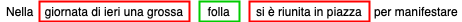
\includegraphics[scale = 0.7]{images/skip-gram.png}
    \caption{Esempio di Skip Gram: in verde il token corrente, in rosso la finestra di contesto grande 5 token.}
    \label{skipgram}
\end{figure}
Per esempio, come illustrato in Figura~\ref{skipgram}, se \textit{folla} è il token corrente, con $m = 5$ il confronto avviene con \{\textit{giornata}, \textit{di}, \textit{ieri}, \textit{una}, \textit{grossa}, \textit{si}, \textit{è}, \textit{riunita}, \textit{in}, \textit{piazza}\}.

L'idea è quella di cercare di costruire il mapping tra $X$, i token correnti (ad esempio \textit{folla}), e $y$, i token estratti dalla finestra di contesto (per esempio \textit{piazza}).

Seguendo la notazione tipica di un problema di apprendimento supervisionato, i token presi dalla finestra di contesto sono la variabile target da predire, apprendendo il tipo di relazione che sussiste tra  $X$ e $y$.
Per farlo, come accennato in precedenza, si utilizza una rete neurale, passando la rappresentazione one-hot del dato a un'unità softmax\footnote{Softmax è una possibile funzione di attivazione dello strato di output della rete neurale. In realtà, vale la pena menzionare altre due varianti di criteri di addestramento applicabili, come Negative sampling e Hierarchical Softmax, con diverse implicazioni riguardo efficienza e onere computazionale.}, una funzione che permette di calcolare la distribuzione di probabilità dei valori possibili nella classificazione multi-classe.

\paragraph{CBOW}
Dualmente a Skip-Gram, CBOW si occupa di predire il token corrente a partire dalla finestra di contesto.

Come mostrato in Figura~\ref{cbow}, si predice con quale probabilità si ottenga il token \textit{folla} a partire dalla finestra \{\textit{giornata}, \textit{di}, \textit{ieri}, \textit{una}, \textit{grossa}, \textit{si}, \textit{è}, \textit{riunita}, \textit{in}, \textit{piazza}\}.
\begin{figure}
    \centering
    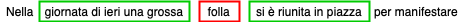
\includegraphics[scale = 0.7]{images/cbow.png}
    \caption{Esempio di CBOW: in rosso il token corrente, in verde la finestra di contesto grande 5 token.}
    \label{cbow}
\end{figure}
Anche in questo caso viene addestrata una rete neurale utilizzando il metodo del gradiente discendente per ottenere l'embedding.
\\
\\
In generale, data la natura di queste tecniche, per ottenere una rappresentazione compatta dell'intero documento si rende necessario l'utilizzo di una tecnica di aggregazione.
In questa fase ogni documento $i$ è formato da $n_i$ parole ed ogni parola è rappresentata da un vettore di $h$ feature. L'aggregazione interviene per comprimere ciascuno di questi vettori in un valore che sia rappresentativo della corrispondente parola, ottenendo, così, un vettore per l'intero documento.

Così come in tante altre applicazioni dell'informatica, i metodi di aggregazione sono molteplici, ad esempio la media aritmetica, la mediana, l'aggregazione del kernel di Fisher \cite{19}.

Fare la media tra vettori significa poter agire su due dimensioni: una di queste prevede di sommare prima gli elementi di ciascun vettore e poi di dividere per il numero di elementi, ottenendo $n_i$ valori medi. In realtà, questa soluzione è scomoda per la successiva elaborazione dei dati, dal momento che ogni documento $i$ può avere un numero variabile di parole e, dunque, si otterrebbero vettori di lunghezza diversa per il corpus finale.

La soluzione utilizzata, invece, consiste nel sommare i primi elementi di tutti i vettori, i secondi, i terzi e così via, per poi dividere per il numero di parole. Così facendo si preserva la rappresentazione tramite feature, perché si ottiene per ogni documento un vettore lungo $h$; un discorso analogo vale per la mediana.

L'aggregazione del kernel di Fisher, invece, propone una rappresentazione che si basa su quanto il vettore osservato si discosti dal modello generativo GMM (Gaussian Mixture Model) \cite{37}. Tale discostamento è una misura di distanza che viene calcolata tramite il gradiente di una funzione di verosomiglianza; i vettori ottenuti prendono il nome di \textit{Fisher vectors}.

\subsubsection{Doc2Vec} \label{d2v}
Doc2Vec nasce come evoluzione di Word2Vec: in questo caso, anziché lavorare a livello di ogni singola parola, si determina direttamente una rappresentazione vettoriale per l'intero documento \cite{24}.
Questo comporta chiaramente il raggiungimento del risultato senza ricorrere a un metodo di aggregazione dei valori.

Conosciuto anche come \textit{Paragraph Vector}, Doc2Vec si articola in due principali implementazioni: \textit{PV-DM} (Distributed Memory) e \textit{DBOW} (Distributed Bag of Words).

\paragraph{PV-DM} 
Come per Word2Vec, il task che viene fatto ripetutamente è quello di predire la parola successiva nella frase. I vettori delle parole e i vettori dei capoversi sono chiamati a contribuire a tale predizione.

Ogni capoverso viene mappato in un vettore, rappresentato da una colonna nella matrice $D$, così come il vettore di ogni parola è rappresentato da una colonna della matrice $P$ (Figura~\ref{pvdm}). I vettori menzionati vengono mediati o concatenati e, a loro volta, essi vengono passati alla rete neurale per prevedere la parola centrale.

La rappresentazione del capoverso è ciò che effettivamente distingue questa tecnica da Word2Vec in quanto, pur agendo come un'altra parola, svolge il ruolo di memoria per ricordare cosa manca al contesto corrente; da qui, il nome \textit{Distributed Memory}.
\begin{figure}
    \centering
    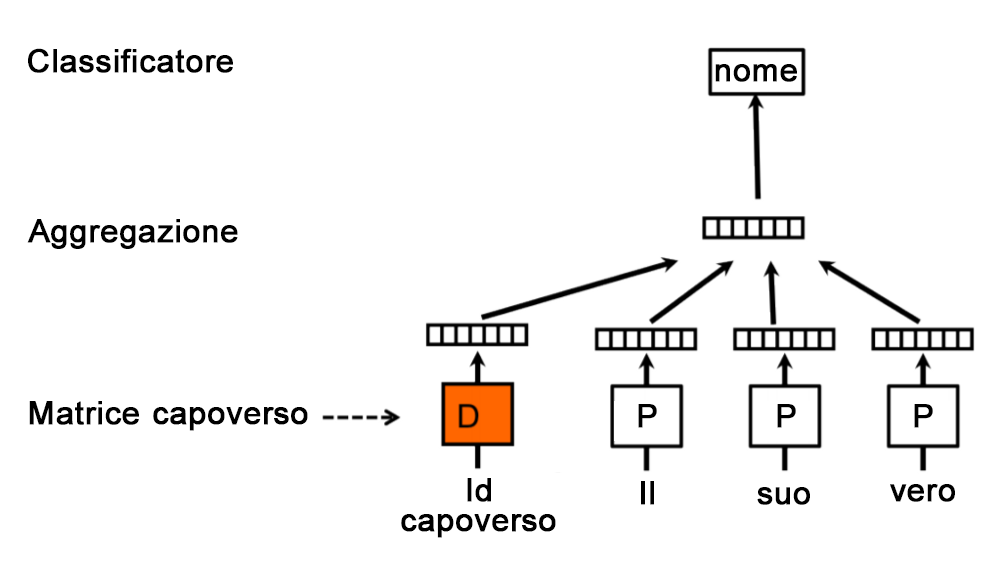
\includegraphics[scale = 0.3]{images/pvdm.png}
    \caption{Architettura in PV-DM (D è la matrice dei documenti e P la matrice delle parole).}
    \label{pvdm}
\end{figure}
La matrice del capoverso ha, infatti, gli embedding per i capoversi ``visti'', allo stesso modo in cui i modelli Word2Vec apprendono gli embedding per le parole. Per i capoversi non visualizzati, invece, il modello viene nuovamente eseguito più volte attraverso la discesa del gradiente per generare un vettore del documento. 

\paragraph{DBOW}
L'architettura DBOW non utilizza le parole di contesto ma effettua la predizione direttamente dalle parole campionate dal capoverso.
\begin{figure}
    \centering
    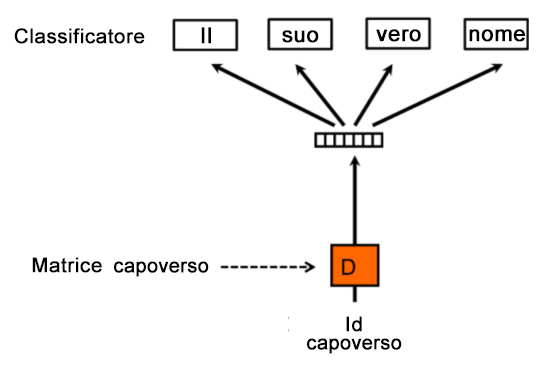
\includegraphics[scale = 0.45]{images/dbow.png}
    \caption{Architettura in DBOW.}
    \label{dbow}
\end{figure}
Ne risulta un'architettura (Figura~\ref{dbow}) simile a PV-DM ma con il primo livello costituito unicamente dalla matrice dei capoversi.

\section{Insiemi fuzzy} \label{insiemifuzzy}
Dal momento che questa tesi si pone l'obiettivo di analizzare le notizie e, nello specifico, di valutare un criterio per individuare quelle fake, è importante introdurre il concetto degli \textit{insiemi fuzzy}.

Diversamente da quanto accade per gli insiemi classici in cui l'appartenenza  è un concetto binario che viene espresso da un valore di verità, negli insiemi fuzzy esso viene quantificato da un valore continuo tra 0 e 1.
Tale valore prende il nome di \textit{grado di appartenenza}.

In altre parole, gli insiemi fuzzy introducono un significato associato all'appartenenza a un insieme che è più granulare rispetto alla tradizionale dicotomia binaria degli insiemi classici, ottenendo valori che indicano anche se una certa espressione sia molto vera, poco vera o mediamente vera.

Nel campo della Sentiment Analysis \cite{25}, per esempio, cercare di determinare le emozioni contenute in un testo rientra in questo tipo di problemi; sarebbe limitante, infatti, considerare unicamente se un tweet o un post esprima felicità o meno, oppure se sia vero o falso che ci sia rabbia nelle parole del messaggio di una persona.

Più realisticamente, esistono componenti più o meno forti di ciascuna di queste emozioni che si mischiano e che formano, complessivamente, un testo.
Tali misture, inoltre, causano spesso dell'incertezza che, di fatto, è la ragione per cui il problema risulta più complesso e, allo stesso tempo, affascinante.

Vari studi, inoltre, hanno evidenziato come l'ambiguità sia una caratteristica intrinseca del linguaggio umano \cite{26, 27}.
Rimanendo nell'esempio della Sentiment Analysis, la presenza di testi con emozioni ambigue è oggi oggetto di ricerca.

Alla luce di tutto ciò, questa tesi propone di modellare la rilevazione delle fake news come un problema fuzzy, assumendo che le notizie siano associate a insiemi di questo tipo.

L'obiettivo è quello di ricavare un modello di apprendimento supervisionato in grado di produrre il grado di appartenenza a tale insieme a partire dal suo contenuto, con l'ambizione finale di ottenere un punteggio di affidabilità per ogni notizia;
potenzialmente, tale punteggio rappresenta quanto la notizia sia fake. Da questo punto di vista è stato fatto un lavoro simile \cite{35} che si basa su un approccio fuzzy ma che ricava l'affidabilità del contenuto a partire dalla fonte dell'informazione.

\section{Induzione di funzioni di appartenenza} \label{induzione}
In letteratura è stato proposto un algoritmo che fa uso di una procedura originariamente nata come tecnica di support vector clustering per poter indurre la funzione di appartenenza dei punti a un certo insieme fuzzy \cite{1}.

I punti fondamentali di questo approccio riguardano determinare la forma di tale insieme fuzzy e inferire i parametri della sua funzione di appartenenza.

\subsection{Funzione di appartenenza} \label{membership}
Il concetto di funzione di appartenenza si colloca nella teoria degli insiemi e corrisponde alla funzione caratteristica di un insieme.

Fissando l'insieme $A$ e lo spazio $X$, la sua funzione di appartenenza $\mu_A$ tale che $Dom(\mu_A) = X$ è definita come:
\begin{equation}
    \mu_A(x)= \begin{cases} 1 & \mbox{se } x \in A, \\ 0 & \mbox{altrimenti.} \end{cases}
\end{equation}
Secondo la teoria classica degli insiemi, infatti, un insieme è definito come qualunque aggregato (o collezione) di oggetti per il quale sia sempre possibile decidere se un generico oggetto appartiene oppure no all'aggregato stesso\footnote{In realtà, questa definizione è stata dimostrata come fallace verso la fine del XIX secolo con quella che venne definita la \textit{crisi dei fondamenti della matematica}. Tale crisi produsse una serie di paradossi, tra cui il famoso \textit{paradosso di Russell} da cui venne derivato il \textit{paradosso del barbiere}. Per rigorosità, sarebbe più opportuno usare una definizione assiomatica degli insiemi, tuttavia, al fine di non rendere prolisso il richiamo alla notazione insiemistica classica, è stata preferita una definizione informale.}.

Quando la funzione di appartenenza è booleana, perché si basa su due soli possibili valori (0 o 1), si parla di insieme \textit{crisp}. Nell'ambito delle notizie, questo corrisponderebbe a classificare ogni notizia come completamente fake o no, a seconda del fatto che appartenga all'insieme delle notizie false.

Lo scopo di questo lavoro, invece, è di rappresentare lo stesso concetto ma in maniera sfumata, producendo informazioni su \textit{quanto} una notizia sia falsa.
Tale rappresentazione ha il vantaggio di poter indicare se una notizia sia più o meno fake di un'altra.
Per questa ragione si introduce il concetto di \textit{grado di appartenenza} con l'idea di base che il confine tra oggetti appartenenti e non appartenenti all'insieme non sia così ben definito.

Ci si concentra, quindi, su una funzione di appartenenza $\mu_A: X \rightarrow [0,1]$ che associa a ogni elemento dell'universo considerato un numero reale compreso tra 0 e 1, dove $X$ è il dominio di $\mu_A$.

Formalmente, si può asserire che:
\begin{itemize}
    \item se $\mu_A(x) = 1$ allora $x$ appartiene all'insieme $A$,
    \item se $\mu_A(x) = 0$ allora $x$ non appartiene all'insieme $A$,
    \item se $0 < \mu_A(x) < 1$ allora $x$ appartiene parzialmente ad $A$ con grado espresso da $\mu_A(x)$.
\end{itemize}
Esempi di concetti fuzzy sono \textit{giovane}, \textit{ricco}, \textit{alto}, mentre non lo sono \textit{fratello}, \textit{studente}, \textit{professore}.

Per determinare il valore di $\mu_A$ vengono definiti diversi tipi di funzioni di appartenenza: funzione sigma, funzione triangolare, trapezoidale, S-Shape, e altre ancora (Figura~\ref{membership_functions}). 
\begin{figure}
    \centering
    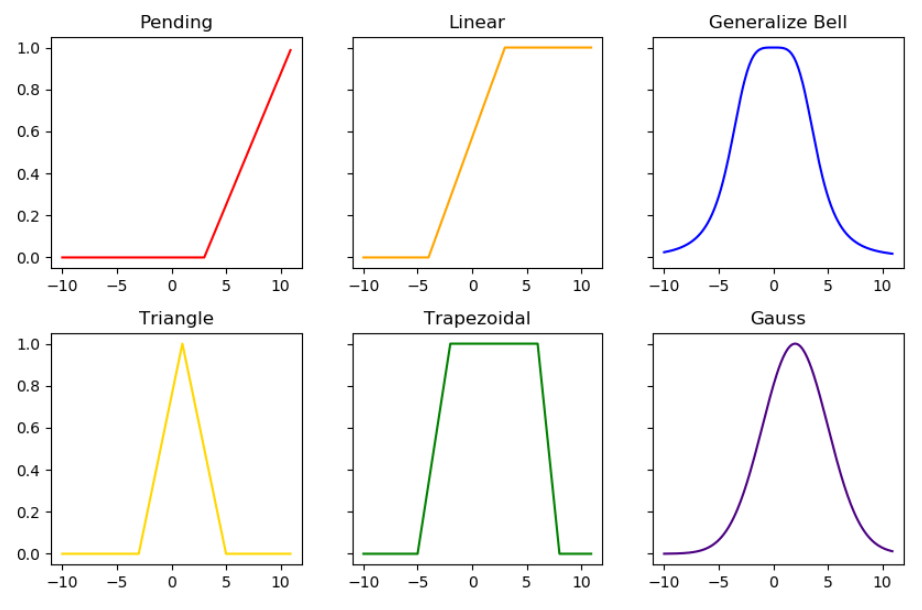
\includegraphics[scale = 0.7]{images/membership_functions.png}
    \caption{Alcuni tipi diffusi di funzioni di appartenenza - da \cite{30}.}
    \label{membership_functions}
\end{figure}
\subsection{Metodi kernel} \label{kernel}
I metodi kernel sono degli oggetti matematici ampiamente utilizzati in congiunzione con le support vector machine \cite{28} per problemi di natura non lineare, tuttavia è applicabile anche a numerosi altri contesti, ad esempio la \textit{kernel Principal Component Analysis} \cite{29}.

Questa metodologia prende il nome di \textit{kernel trick} e consiste nel mappare i punti dallo spazio originale $\mathcal X$ a uno spazio $\mathcal H$ a dimensionalità superiore o infinita, dove il problema diventa lineare e i dati risultano linearmente separabili.
Tale tecnica si appoggia a una funzione kernel, una funzione simmetrica 
\begin{equation}
    k: \mathcal{X} \times \mathcal{X} \rightarrow \mathbb{R}
\end{equation} 
tale che in $\mathcal{H}$, detto \textit{spazio delle feature}, è definito un prodotto scalare $<$ ·, · $>$ ed esiste una funzione $\mathit{\Phi }: \mathcal{X} \rightarrow \mathcal{H}$ per cui:
\begin{equation}
    k(x,y) = <\mathit{\Phi}(x), \mathit{\Phi}(y)>
\end{equation}
dove $x,y \in \mathcal{X}$.
I dati vengono, quindi, rappresentati tramite dei confronti di coppie, misurando l'equivalente di una misura di similarità: all'aumentare di $k(x,y)$, $x$ e $y$ sono da considerarsi maggiormente  ``simili''.
Inoltre, tramite l'utilizzo di questo metodo, la dimensionalità dei dati tende a diventare poco influente, ragione per cui, spesso, metodi come questi non soffrono della \textit{maledizione della dimensionalità} \cite{39}.
Esistono diversi tipi di kernel, ad esempio lineare, polinomiale, iperbolico, gaussiano e molti altri ancora.

\subsection{Tipi di kernel}
In letteratura è presente un'importante varietà di kernel ed essi si distinguono per il tipo di funzione $k(x,y)$ utilizzata. Seguono, dunque, alcuni esempi dei kernel più diffusi:

\paragraph{Kernel lineare}
Il kernel lineare usa la funzione
\begin{equation}
    k(x,y) = x \cdot y = \sum\limits_{i=1}^n x_iy_i
\end{equation}
dove $n$ è la dimensione comune di $x$ e $y$.
La proiezione dell'iperpiano dallo spazio $\mathcal{H}$ allo spazio $\mathcal{X}$ corrisponde a un iperpiano.

\paragraph{Kernel polinomiale}
Il kernel polinomiale usa la funzione
\begin{equation}
    k(x,y) = (x \cdot y + 1)^d
\end{equation}
dove $d$ è il grado polinomiale del kernel.
In questo caso l'iperpiano equivale a una superficie polinomiale di grado al più $d$.

\paragraph{Kernel polinomiale omogeneo}
Il kernel polinomiale omogeneo usa la funzione
\begin{equation}
    k(x,y) = (x \cdot y)^d
\end{equation}
dove $d$ è il grado polinomiale del kernel. La proiezione dell'iperpiano, qui, corrisponde a una superficie polinomiale di grado esattamente uguale a $d$.

\paragraph{Kernel gaussiano}
Il kernel gaussiano usa la funzione
\begin{equation}
    k(x,y) = e^{-\frac{||x-y||^2}{2\sigma^2}}
\end{equation}
dove $\sigma$ è la deviazione standard. Questo tipo di kernel è una combinazione lineare di infiniti kernel polinomiali di grado crescente. Lo spazio delle feature indotto dal kernel gaussiano, infatti, è dimensionalmente infinito. L'iperpiano in tale spazio equivale nello spazio originale a una sovrapposizione di curve gaussiane, la cui deviazione standard è regolata da $\sigma$.

\paragraph{Kernel basato su tangente iperbolico}
Il kernel basato su tangente iperbolico usa la funzione
\begin{equation}
    k(x,y) = \tanh(\alpha x \cdot y + \beta)
\end{equation}
dove $\alpha$ e $\beta$ sono rispettivamente i parametri di scala e offset. La funzione in questione ha origine nell'ambito delle reti neurali; si osserva, inoltre, che un modello basato su support vector machine che usa questa funzione di attivazione sia equivalente a una rete neurale feedforward a due strati.

\chapter{Soluzione proposta}
\label{Capitolo 2}
\onehalfspacing
Questo capitolo presenta la soluzione che viene proposta in questa tesi.
Tale soluzione consiste in un sistema di apprendimento supervisionato a partire dall'algoritmo $\bm{\mu}$\textbf{-learn} \cite{1}, il cui funzionamento viene descritto nel Paragrafo~\ref{mulearn}.

Segue nel Paragrafo~\ref{evaluation} l'illustrazione dei criteri di valutazione dei modelli e nel Paragrafo~\ref{generalization} la maniera con cui viene misurata la loro bontà di generalizzazione.

Nel Paragrafo~\ref{sistema}, invece, si mostra l'utilizzo che è stato fatto dell'algoritmo sopracitato all'interno del sistema proposto in questo capitolo, delineando le fasi che si susseguono nel corso degli esperimenti. Infine nel Paragrafo~\ref{predictors} vengono mostrati i due tipi di predittore che sono stati proposti per tali esperimenti.

\section[\texorpdfstring{L'algoritmo $\mu$-learn}%
                        {mu-learn}]% % choose text-only material here
        {L'algoritmo $\bm{\mu}$-learn}  % note use of \bm ("bold math")
\label{mulearn}
$\mu$-\textit{learn} è un algoritmo di Machine Learning supervisionato che utilizza una procedura originariamente nata nel contesto del support vector clustering~\cite{23}.
Essa si colloca nel gruppo di tecniche che lavora su insiemi fuzzy, trattando un problema di ottimizzazione non lineare.

La diversità delle funzioni di appartenenza presenti in letteratura permette una vasta sperimentazione e i parametri associati a tali funzioni possono essere regolati in modo da ottenere forme differenti per gli insiemi fuzzy formati.
Il nome di questo algoritmo suggerisce il suo obiettivo: apprendere $\mu$, la funzione di appartenenza a un determinato insieme fuzzy e generare l'associato modello predittivo.

\subsection{Support vector clustering modificato}\label{svcmodified}
L'assunzione iniziale è quella di disporre di un dataset $S$ di $m$ osservazioni tale che
\begin{equation}
    S = \{(\mathbf{x_i}, y_i), \; \forall\,i=1, ..., m\}
\end{equation}
in cui $\mathbf{x_i} \in \mathbb{R}^h$ è l'$i$-esimo vettore delle feature e $y_i$ è l'etichetta target che si vuole predire; tale etichetta può essere rappresentata da dei valori binari in $[0,1]$ o dai gradi di appartenenza $\mu_i$ a un insieme fuzzy sconosciuto $A$.
L'obiettivo è proprio individuare tale insieme e determinare la funzione di appartenenza $\mu_A$ per approssimarne il grado.

L'algoritmo descritto nel Paragrafo~\ref{mulearn} parte dalla tecnica di support vector clustering presente in letteratura~\cite{23} e la estende per l'individuazione di insiemi fuzzy. Si tratta di un algoritmo di clustering non parametrico che affronta il problema dell'identificazione del minimo raggio dell'ipersfera di raggio $R$ e centro $a$ che include le immagini della maggior parte di un insieme di punti; in particolare, i punti che si trovano sulla superficie di tale ipersfera sono chiamati \textit{support vector} e, nello spazio delle feature, essi dividono i dati in cluster.
Tali punti vengono esclusi o inclusi da $\mu$-learn in funzione dei loro gradi di appartenenza a un insieme fuzzy, sulla base della distanza tra le immagini dei punti e $a$.

Il problema di ottimizzazione non lineare a cui si accennava nel Paragrafo~\ref{mulearn} riguarda, quindi, la minimizzazione del raggio di questa ipersfera.

Quelli che seguono sono i tre vincoli del problema e si distinguono dalla tecnica originale proprio per l'introduzione di $\mu_i$:
\begin{equation}\label{vincolo}
    \mu_i || \mathit{\Phi}(x_i) - a ||^2 \leq \mu_iR^2 + \xi_i \;,
\end{equation}
\begin{equation}\label{vincolo_2}
    (1 - \mu_i) || \mathit{\Phi}(x_i) - a ||^2 \geq (1 - \mu_i)R^2 - \tau_i \;,
\end{equation}
\begin{equation}\label{vincolo_3}
    \xi_i \geq 0, \tau_i \geq 0 \;.
\end{equation}
In~\ref{vincolo} il primo vincolo richiede che le immagini dei punti attraverso $\mathit{\Phi}$ abbiano una distanza dal centro minore o uguale di una quantità che è tanto più piccola quanto più è elevato il relativo $\mu_i$. Il secondo vincolo in~\ref{vincolo_2} richiede, invece, che al diminuire di $\mu_i$, le immagini si trovino a una distanza che tende ad aumentare. Infine, il vincolo~\ref{vincolo_3} impone dei valori non negativi per le variabili slack che rilassano il problema.

Il problema di ottimizzazione originale viene, quindi, esteso minimizzando $R^2 + C\sum(\xi_i + \tau_i)$ tramite (\ref{vincolo}-\ref{vincolo_3}), dove $C$ è un iperparametro, e viene ricavata tramite un solver.
La fase successiva è quella di indurre il valore della funzione di appartenenza a tale insieme.

\subsection{Fuzzificatore} \label{fuzzificatore}
In letteratura i termini \textit{fuzzificazione} e \textit{defuzzificazione} indicano rispettivamente il passaggio da una quantità crisp a una quantità fuzzy e viceversa.
Tale passaggio può avvenire in differenti modi che dipendono dal tipo di fuzzificatore che si utilizza. 
In altre parole, si stabilisce il modo in cui vengono fatti decrescere i valori della funzione di appartenenza dal valore 1 fino a 0. Geometricamente, questo equivale a definire una certa misura di distanza nello spazio in cui i punti vengono racchiusi; con grado di appartenenza maggiore essi saranno raggrupati più densamente nell'ipersfera di cui l'algoritmo minimizza il raggio, dualmente con grado minore, i suddetti punti saranno più distanti dall'insieme.
Nel caso di $\mu$-learn, sono stati implementati diversi tipi di fuzzificatore, ciascuno caratterizzato dall'apprendimento di un diverso profilo della funzione di appartenenza. Per profilo si intende la funzione associata 
\begin{equation}
    p: \mathbb{R}^+ \rightarrow [0,1]
\end{equation}
che ritorna i gradi di appartenenza a partire dai suoi argomenti nello spazio delle feature. Ogni tipo di fuzzificatore determina, quindi, una specifica distribuzione per $p$.

\paragraph{Fuzzificatore crisp}
Il fuzzificatore crisp usa una funzione basata su soglia $r_{crisp}$ che viene tipicamente posta uguale al quadrato del raggio della sfera appresa o indotta tramite interpolazione.
\begin{equation}
    p(r)= \begin{cases} 1 & \mbox{se } r \leq r_{crisp}, \\ 0 & \mbox{altrimenti.} \end{cases}
\end{equation}

\paragraph{Fuzzificatore lineare}
In questo tipo di fuzzificatore, il grado di appartenenza descresce linearmente, per cui
\begin{equation}
    p(r)= \begin{cases} 1 & \mbox{se } r \leq r_1, \\l(r) & \mbox{se } r_1 \leq r \leq r_0 \\ 0 & \mbox{altrimenti.} \end{cases}
\end{equation}
in cui $l$ è una funzione lineare.

\paragraph{Fuzzificatore esponenziale} Il grado di appartenenza, in questo caso, viene fatto decrescere esponenzialmente tramite una funzione esponenziale $e$
\begin{equation}
    p(r)= \begin{cases} 1 & \mbox{se } r \leq r_1, \\e(r) & \mbox{altrimenti}. \end{cases}
\end{equation}

\paragraph{Fuzzificatori a tratti basati su quantili} Sono stati, inoltre, implementati dei fuzzificatori basati su quantili, sia nella variante costante che in quella lineare.
In questo caso gli step della funzione sono definiti in funzione dei quartili delle distanze quadratiche tra le immagini dei punti e il centro della sfera appresa.

\subsection{Induzione di insiemi fuzzy}
Se $F$ è l'insieme fuzzy analizzato, l'algoritmo descritto nel Paragrafo~\ref{mulearn} individua $K$, detto \textit{core}, ovvero l'insieme crisp di tutti i punti che hanno membership unitaria di appartenenza a F. Sulla base del fuzzificatore impostato (Paragrafo~\ref{fuzzificatore}), poi, l'algoritmo fa decrescere il valore di appartenenza previsto man mano che i punti si allontanano dal core. 
Al fine di visualizzare il comportamento descritto, si mostra in Figura~\ref{mulearnplot} un esempio di esecuzione dell'algoritmo e la conseguente rappresentazione del risultato ottenuto:
si assuma che le fake news siano appartenenti a un determinato insieme fuzzy $F$ e si supponga di volerlo individuare tramite la procedura vista in precedenza.
Con un campione di 400 notizie (228 vere e 172 fake) opportunamente preprocessato con le tecniche viste nel Paragrafo~\ref{nlp}, è stato eseguito $\mu$-learn con un kernel gaussiano e un fuzzificatore di tipo lineare; successivamente, i risultati sono stati rappresentati in uno spazio bidimensionale applicando la tecnica di PCA~\cite{30}.

Considerando che i punti rossi fanno riferimento alle osservazioni etichettate come fake news e quelli blu alle notizie vere, si osserva la formazione di diverse \textit{curve di livello} che descrivono i gradi di appartenenza a $F$ in prossimità della zona in cui i punti rossi sono maggiormente concentrati.

Man mano che ci si avvicina alle zone periferiche il grado viene diminuito linearmente rispettando i valori delle curve di livello.
\begin{figure}
    \centering
    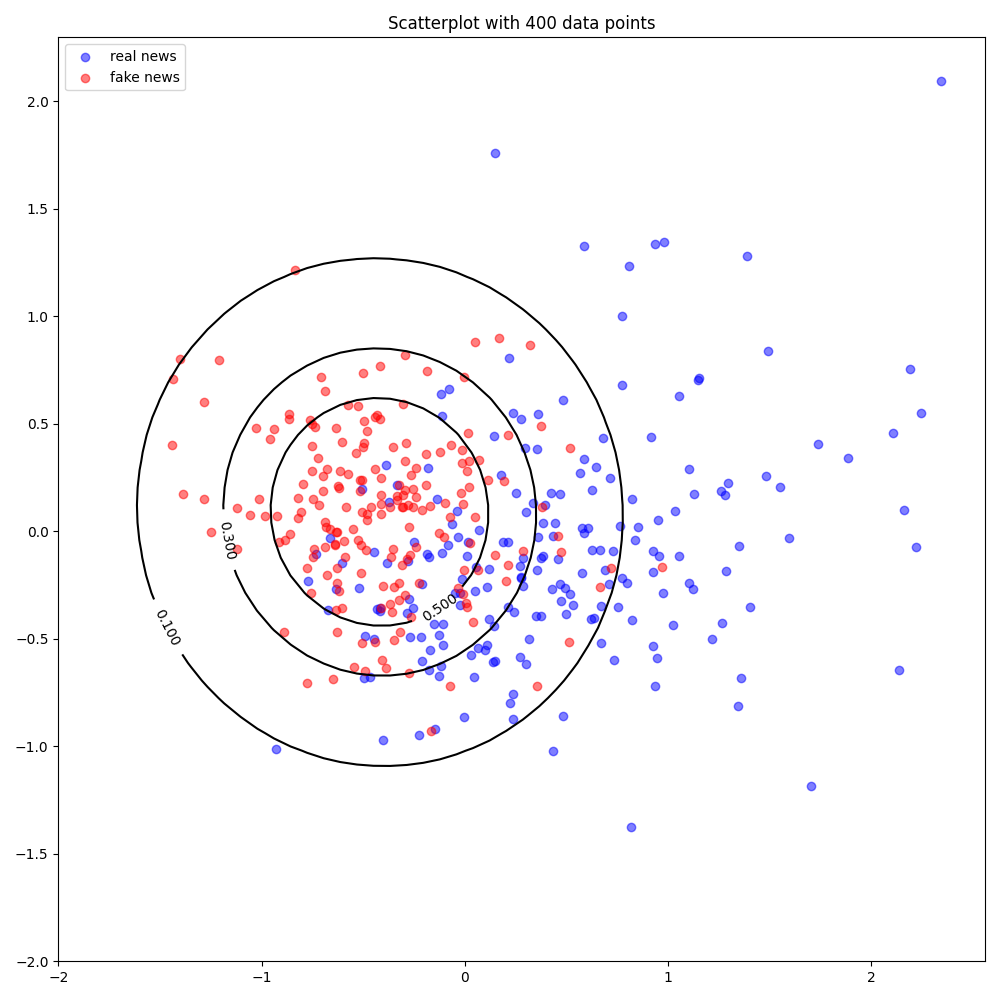
\includegraphics[scale=0.44]{images/mulearn.png}
    \caption{Visualizzazione in uno spazio bidimensionale dei punti (400 osservazioni) e del fuzzy set associato alle fake news indotto da $\mu$-learn. In rosso le notizie echitettate come ``fake'' e in blu come ``vere''.
    Le curve di livello discriminano i gradi di appartenenza dei punti a partire dall'insieme core al centro fino al resto delle osservazioni nelle zone periferiche.}
    \label{mulearnplot}
\end{figure}
La fase di induzione della funzione di appartenenza è lo step in cui l'algoritmo viene effettivamente addestrato tramite i dati etichettati.

L'esito dell'induzione della funzione di appartenenza è influenzato dalla scelta degli iperparametri, che vengono descritti nel paragrafo successivo.

\subsection{Iperparametri}\label{iperparameters}
Gli \textit{iperparametri} sono parametri speciali che non vengono appresi direttamente dall'algoritmo di Machine Learning, al contrario, il loro valore viene assegnato prima dell'addestramento.
Nel contesto considerato da questa tesi si distinguono i seguenti iperparametri: 
\begin{enumerate}
    \item il solver utilizzato,
    \item il tipo di kernel,
    \item eventuali parametri che dipendono dal tipo di kernel,
    \item il parametro di regolarizzazione $C$,
    \item il tipo di fuzzificatore,
    \item eventuali parametri legati al tipo di fuzzificatore.
\end{enumerate}
Nella soluzione proposta in questa tesi, tra le svariate possibilità esistenti, è prevista la scelta tra due solver: \textit{tensorflow} e \textit{gurobi}, che usano strategie differenti per il problema di ottimizzazione non lineare. Il secondo e il terzo iperparametro condizionano indirettamente la forma dell'insieme indotto.

Il parametro $C$ impatta sulla dimensione del core dell'insieme:
all'aumentare di $C$, il core si dilata e incrementa il numero di elementi in esso inclusi.
Inoltre, è stato osservato sperimentalmente che, al raggiungimento dell'unità da parte di $C$, l'insieme fuzzy tende a un insieme regolare che racchiude i punti del campione le cui etichette sono diverse da zero.

Infine, il quinto e il sesto iperparametro sono legati al processo di fuzzificazione precedentemente definito nel Paragrafo~\ref{fuzzificatore}.
Una volta individuato un insieme di valori per ogni iperparametro, è possibile ricorrere a una tecnica per la ricerca dei loro valori ottimali, detta \textit{tuning}.

\paragraph{Tuning} Con tuning si intende l'addestramento di uno stimatore con diverse configurazioni dei suoi iperparametri, al fine di valutare i risultati delle predizioni e, sulla base di essi, scegliere opportunamente il set di valori ottimali per la generazione del modello finale.

Nella soluzione proposta in questa tesi, la fase di tuning è stata concretamente implementata tramite la cosiddetta \textit{grid search}: si tratta di una ricerca del modello migliore che considera una tabella di valori che si desidera esplorare e si basa sulla suddivisione del campione dei dati in \textit{training set}, \textit{validation set} e \textit{test set}.
Questi tre tipi di insieme vengono ricavati dal dataset a disposizione mantenendo la composizione denotata nel Paragrafo~\ref{svcmodified}, ovvero formati da coppie di vettori di feature e di etichette. Essi si differenziano tra loro per il diverso scopo al quale ciascuno è dedicato: i dati del training set vengono utilizzati per l'addestramento, il validation set serve a valutare la bontà delle predizioni ed eventualmente regolare gli iperparametri per ottenere risultati migliori. Il test set, invece, serve per testare il modello finale così da trarre le relative conclusioni.
In generale, è importante che ciascuno di questi insiemi, così come il dataset di partenza, siano rappresentativi\footnote{Per dataset rappresentativo si intende un campione sufficientemente popolato e possibilmente bilanciato.} del dominio che si intende considerare.

L'algoritmo viene configurato con ogni combinazione della grid search, generando per ciascuna un modello che viene addestrato col training set, un insieme di dati etichettati necessari per formare la memoria del modello predittivo. Successivamente, il modello osserva i dati del validation set, cioè nuove osservazioni del campione che permettono di fare un confronto con le relative previsioni fatte dal modello indotto. Tali predizioni vengono, dunque, comparate alle etichette originali per misurare la capacità predittiva del modello; questo viene fatto tramite delle apposite metriche e, sulla base di queste, si sceglie il modello effettivamente più efficace.

Il test set, invece, funge da prova finale per valutare la capacità di generalizzazione del modello su dati mai visti, valutando la bontà delle sue predizioni su di essi.
Esistono tanti modi per dividere i dati nei tre insiemi sopra descritti, uno di questi è la \textit{cross validation}.


\paragraph{Cross validation} 
La cross validation è una tecnica che consiste nel partizionare il dataset in $k$ \textit{fold} equiampie, effettuare altrettante iterazioni e, per ciascuna, considerare l'$i$-esima fold come validation set e le restanti $k-1$ come training set per addestrare il modello generato.
In questo caso esistono diverse scuole di pensiero sulla percentuale che si preferisce impostare per la suddivisione in fold.
In generale, è opportuno bilanciare le fold in maniera tale da avere un numero sufficiente di dati per fare l'apprendimento e per fare la validazione.

Indirettamente, definire ogni combinazione delle fold equivale a definire un nuovo modello, pertanto fare una cross validation $k$-fold significa generare $k$ modelli.

Questa tecnica ha il vantaggio di massimizzare l'utilizzo dei dati, utilizzando a turno ogni fold come validation set e, dunque, consentendo di eseguire l'algoritmo su più casi.

In realtà, la stessa tecnica può essere utilizzata per ottenere anche i test set legati alla valutazione della generalizzazione; in questo caso, però, è necessario fare quella che viene definita \textit{cross validation annidata}.

\paragraph{Cross validation annidata}
La cross validation annidata è un'estensione della versione riportata nel precedente capoverso e può essere usata per ricavare diversi test set. Quest'operazione viene fatta eseguendo un'ulteriore cross validation interna per ciascuna delle $k$ fold, ottenendo $l$ fold interne. A questo punto la validazione del modello viene spostata alle fold interne, in cui si opera la ricerca degli iperparametri ottimali, mentre quelle esterne consentono di testare il modello.

\section{Valutazione dei modelli}\label{evaluation}
La scelta dei modelli si basa sull'utilizzo di uno o più criteri di valutazione. Il range di possibilità esistenti in questo senso è molto ampio e la motivazione che porta a preferire una soluzione piuttosto che un'altra dipende strettamente dal tipo di problema considerato, così come dal tipo di dati a disposizione: nell'ambito della classificazione, ad esempio, si ragiona in termini di accuratezza, ossia la percentuali di predizioni corrette rispetto a quelle totali; in un contesto differente, come ad esempio quello della regressione, non è più possibile basare la bontà di un modello sull'accuratezza, poiché entra in gioco quella che è la quantificazione dell'errore. L'errore è una misura del discostamento che si verifica tra una predizione e la ground truth, ossia l'effettivo valore delle etichette nel dominio di conoscenza considerato.
La differenza è che, mentre un classificatore (binario) può commettere solo due tipi di errore\footnote{Generalizzando, un classificatore $n$-ario può commettere $n(n-1)$ diversi tipi di errore.}, denominati \textit{falsi positivi} e \textit{falsi negativi}, nel caso della regressione l'errore può essere un qualunque numero positivo.
In generale, ricorrere a queste misure consente di descrivere quanto sia rilevante l'errore compiuto dal predittore e stabilire se sia numericamente accettabile per la scelta finale del modello.

\subsection{Matrice di confusione}
Quando si mira ad ottenere un classificatore, uno strumento molto utilizzato per valutare la sua bontà è la matrice di confusione, una struttura dati che analizza le predizioni e le divide nelle quattro classi menzionate nel paragrafo precedente. 
Il caso più semplice è quello mostrato in Figura~\ref{confusion} in cui si considera delle etichette binarie.

Nel contesto di classificazioni multi-classe è sufficiente estendere la matrice ottenendo sulla diagonale il numero di predizioni corrette e nel resto della matrice i vari casi di errore con cui è possibile capire quali classi vengano più o meno facilmente confuse. 

\begin{figure}
    \centering
    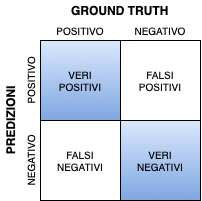
\includegraphics[scale=0.7]{images/confusion matrix.png}
    \caption{Matrice di confusione su classificazione binaria. Nell'ambito considerato in questa tesi la classificazione ``positiva" riguarda il fatto che una notizia sia fake, dualmente quella ``negativa" si riferisce alle notizie vere.}
    \label{confusion}
\end{figure}

\subsection{Precision, Recall e F1}\label{erroreclass}
L'accuratezza è una misura utile ma che assume una distribuzione uniforme delle quattro classi individuate nella matrice di confusione. Nel caso in cui tale distribuzione non sia effettivamente uniforme, questo tipo di misura può risultare ingannevole: si consideri, ad esempio, un campione di 1000 predizioni in cui si ha 1 vero positivo, 0 falsi positivi, 1 falso negativo e 998 veri negativi. In questo caso si otterrebbe un'accuratezza pari a 99.9\% ma, come è facile intuire da questo esempio giocattolo, tale misura non fornisce alcuna informazione riguardo a come le predizioni corrette siano distribuite e questo potrebbe rivelarsi un problema nel momento in cui si confrontano degli esiti così diversi per i casi positivi e per quelli negativi.
Nel contesto della classificazione è possibile, infatti, calcolare delle misure quantitative per valutare la bontà di un predittore che tengono in considerazione la distribuzione delle predizioni; esse sono dette \textit{Precision}, \textit{Recall} e \textit{F1} e sono basate sul numero di veri positivi, veri negativi, falsi positivi e falsi negativi.

\paragraph{Precision}
Il valore di \textit{Precision} misura la frazione di predizioni positive correttamente individuate dal classificatore. Nell'esempio delle fake news si potrebbe interpretare questa misura come la percentuale di notizie classificate come fake che effettivamente sono false.
\begin{equation}
\frac{\text{Veri Positivi}}{\text{Veri Positivi} + \text{Falsi Positivi}}
\end{equation}

\paragraph{Recall}
La \textit{recall} quantifica il numero di predizioni positive corrette rispetto a tutte le osservazioni positive. Ricollegandosi alle fake news, la recall rappresenterebbe la percentuale di tutte le notizie fake del dataset che sono state individuate dal classificatore.
\begin{equation}
\frac{\text{Veri Positivi}}{\text{Veri Positivi} + \text{Falsi Negativi}}
\end{equation}

\paragraph{F1}
Dal momento che le precedenti quantità rappresentano due facce della stessa medaglia, il punteggio \textit{F1} nasce con l'intento di combinarle tramite la media armonica.
\begin{equation}
\frac{2 \times (\text{Precision} \times \text{Recall})}{\text{Precision} + \text{Recall}}
\end{equation}

\subsection{MSE e RMSE}\label{erroreregr}
Il concetto di accuratezza di un modello non è sempre applicabile, specialmente se si considera un tipo di predittore che produce valori continui\footnote{Qui il termine ``continui'' è da intendersi da un punto di vista puramente teorico, in quanto a livello informatico si tratta comunque di un intervallo di valori discreto, derivante dalla limitata capcità di memoria di un calcolatore.}. In questi casi si ricorre a delle misure del concetto di \textit{errore}, ossia la quantità che descrive quanto il valore della predizione sia deviato rispetto alla ground truth.
In questa tesi sono state utilizzate le metriche di \textit{mean squared error} e di \textit{root mean squared error}.

Nelle definizioni che seguono, $S$ denota il dataset formato da tutte le coppie $(\mathbf{x_i},y_i)$ con $i=1, ..., m$,
dove $\mathbf{x_i}$ indica il vettore delle feature, $y_i$ l'etichetta, $i$ l'indice di scorrimento delle osservazioni e $m$ è la dimensione del dataset.
\paragraph{MSE} L'errore quadratico medio è definito come
\begin{equation}
    \frac{1}{m}\sum\limits_{j=1}^m (\hat{y_j} - y_j)^2
\end{equation}
dove $\hat{y}_j$ è la predizione.
\paragraph{RMSE}
Al fine di portare il valore dell'errore ad avere la stessa unità di misura delle predizioni può essere utile sfruttare l'RMSE, definito come 
\begin{equation}
    \sqrt{MSE}
\end{equation}

\section{Bontà di generalizzazione di un modello}\label{generalization}
Nell'ambito del Machine Learning, generare un modello predittivo affidabile non significa selezionare semplicemente il modello che ottiene i risultati migliori bensì quello che si adatta meglio ai dati.
Questa capacità di adattamento consente di valutare quella che viene definita la \textit{bontà di generalizzazione} che il modello ha sui dati che non ha mai visto. Da questo punto di vista, un modello con una buona capacità di generalizzazione è in grado di intuire correttamente le etichette dei dati perché è riuscito ad estrarre efficacemente la relazione di dipendenza tra le feature e le etichette target desiderate.
A volte, questo meccanismo viene raggiunto sui dati di addestramento tramite una continua regolazione degli iperparametri nella fase di tuning, tuttavia questo rischia di causare la generazione di un modello che su quel tipo di dato riesce a ottenere buoni risultati ma che ha una bassa capacità di generalizzazione su altri poiché, più che formare la sua esperienza su concrete relazioni dei dati, ha raggiunto l'obiettivo tramite un eccessivo incremento della complessità.

Gli iperparametri determinano, infatti, i gradi di libertà del modello ottenuto e la loro numerosità ha un impatto sulla complessità del modello: avere molti iperparametri rischia di complicarlo eccessivamente, dualmente, averne pochi, lo rende potenzialmente troppo semplice. 
Sulla base di queste premesse si introducono, quindi, i concetti di \textit{overfitting} e \textit{underfitting}.

\subsection{Overfitting e underfitting}
Si distinguono modelli che soffrono di \textit{underfitting} quando hanno errore alto sul training set e sul test set, tipicamente questo è causato da un'eccessiva semplificazione del modello o da una quantità di dati di addestramento insufficiente.

Al contrario, modelli che soffrono di \textit{overfitting} sono troppo complessi e mostrano un errore basso sul training set ma alto sul test set, evidenziando una scarsa capacità di generalizzazione.

In letteratura, il problema è descrivibile anche in termini di equilibrio tra \textit{bias} e \textit{variance error}, derivanti dalla \textit{decomposizione bias-variance}; tale decomposizione descrive le componenti che formano l'errore totale di uno stimatore prodotto da qualsiasi algoritmo di Machine Learning: bias error, variance error e Bayes error.

Il bias error è l'errore costituito dalle ipotesi semplificative fatte da un modello per rendere più facile l'apprendimento della variabile target.

Il variance error è, invece, la quantità che misura quanto cambia la previsione della variabile target al variare dei dati di addestramento.

Infine, il Bayes error è una quantità irriducibile e, dal punto di vista dell'apprendimento automatico, inevitabile; si tratta dell'intrinseco errore introdotto dalla scelta del problema.

Da questo punto di vista, l'underfitting è il risultato del prevalere del bias error sul variance error; l'overfitting, invece, è causato dal dominare del variance error sul bias error.
Di conseguenza, al fine di trovare un compromesso per controllare questo tipo di problematica, è necessario avere una giusta complessità del modello, associata a un campione di dati sufficientemente grande.

In Figura~\ref{underfittingoverfitting} viene riportato un confronto tra due modelli: nell'immagine di sinistra è presente un modello troppo semplice con un eccessivo bias error; a destra, invece, un modello con tanti gradi di libertà allo scopo di adattarsi molto bene ai punti ma che porta ad aumentare il variance error, rivelandosi poco robusto su nuove osservazioni. 
Un altro aspetto che non dipende dalla complessità del modello e a cui, però, occorre prestare comunque attenzione è il fenomeno di \textit{data leakage}.

\begin{figure}
\centering
    \begin{minipage}{0.48\textwidth}
        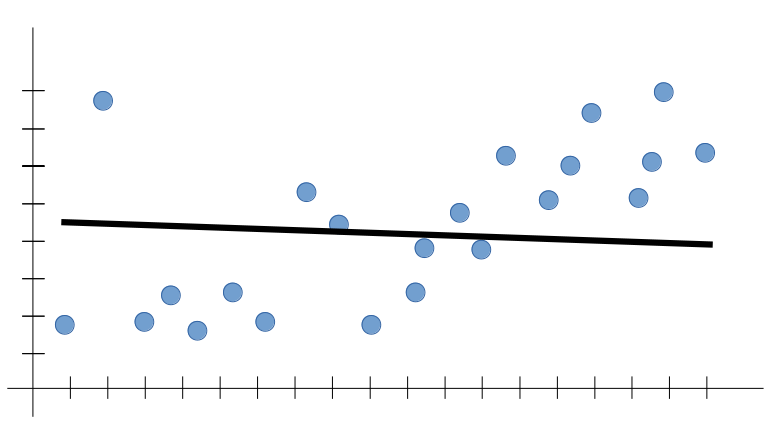
\includegraphics[width=\linewidth]{images/underfitting.png}
    \end{minipage}
    \begin{minipage}{0.48\textwidth}
        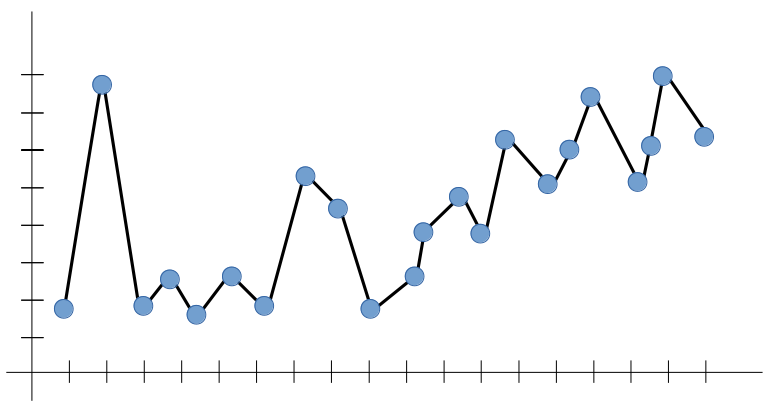
\includegraphics[width=\linewidth]{images/overfitting.png}
    \end{minipage}
    \caption{Nel primo grafico si mostra un esempio di modello di Machine Learning che evidenzia problemi di underfitting; nel secondo caso si mostra un tipico comportamento di overfitting - Fonte: \url{https://towardsdatascience.com/what-are-overfitting-and-underfitting-in-machine-learning-a96b30864690}.}
    \label{underfittingoverfitting}
\end{figure} 

\paragraph{Data leakage} Per \textit{data leakage} si intende lo scenario in cui il training set o il validation set viene contaminato dal test set. In altre parole violare la proprietà di disgiunzione tra questi due tipi di insiemi causa un eccessivo adattamento del modello sui dati di allenamento e, di conseguenza, performa molto bene su questi ultimi ma molto male su osservazioni nuove.
Questa è la ragione per cui il partizionamento del campione in training, validation e test set deve essere fatto rendendo tali insiemi disgiunti fra loro.

\section{Il sistema}
\label{sistema}
In questo paragrafo si mostra ad alto livello l'architettura della soluzione proposta in questa tesi per la rilevazione delle fake news tramite l'induzione di insiemi fuzzy, presentando prima i nodi che la compongono e poi descrivendo come sia stato utilizzato l'algoritmo $\mu$-learn nel contesto del riconoscimento delle fake news.
Nella seconda parte viene, invece, spiegato come i nodi in questione comunichino fra loro e quali file vengano generati durante l'utilizzo del sistema. Sarà, quindi, obiettivo del Capitolo~\ref{Capitolo 3} illustrare più a basso livello l'implementazione del sistema e descrivere nel dettaglio i nodi che vi appartengono.

Per gestire la pluralità dei casi nella forma dell'input, il sistema definisce un formato standard per i dataset che andrà a trattare: il dataset ideale è un dataframe che contiene in forma tabulare osservazioni relative a dati testuali che, nell'ambito trattato da questa tesi, possono essere il corpo delle notizie o i titoli.
Tali osservazioni sono etichettate con valore 1 se si tratta di una notizia fake, 0 altrimenti.

L'obiettivo di $\mu$-learn sarà, quindi, indurre l'insieme fuzzy delle fake news inizialmente sconosciuto ed apprendere la funzione di appartenenza ad esso associata.
\subsection{Architettura}\label{architecture}
L'architettura del sistema è composta da tre nodi, dedicati alle seguenti attività: 
\begin{enumerate}
    \item il preprocessing del dataset,
    \item la selezione dei modelli migliori,
    \item la visualizzazione dei dati.
\end{enumerate}
Segue, quindi, una breve descrizione di ciascun nodo più nel dettaglio.

\paragraph{Preprocessing del dataset} All'inizio di questa fase ci sono tre possibili scenari: i) il dataset rispetta il formato predefinito, ii) il dataset è formattato diversamente e dunque necessita di una fase di rielaborazione per poter essere utilizzabile, iii) il dataset viene generato dal sistema stesso.
In altre parole, nel secondo caso è necessario rendere la forma dell'input compatibile col formato predefinito; questo viene fatto da un modulo che ha la funzione di estrarre le informazioni fondamentali e di formare con esse il dataframe desiderato.
A questo punto interviene la vera e propria fase di preprocessing che consiste nell'eseguire una pipeline di operazioni che hanno l'obiettivo di preparare il dataset alla fase successiva.

Le operazioni in questione includono le tecniche di elaborazione del linguaggio naturale descritte nel Capitolo~\ref{Capitolo 1} e la cui implementazione viene illustrata nel dettaglio nel Capitolo~\ref{Capitolo 3}.

La pipeline che assembla tali operazioni e che le esegue in sequenza viene opportunamente configurata a seconda delle esigenze per attivare o disattivare gli step per l'elaborazione dei dati, anche in base allo scenario considerato.

Al termine del preprocessing, un nuovo dataset viene creato e scritto su file, per il suo utilizzo in un secondo momento. L'intero processo viene schematizzato in Figura~\ref{preprocessmodule}.

\begin{figure}
    \centering
    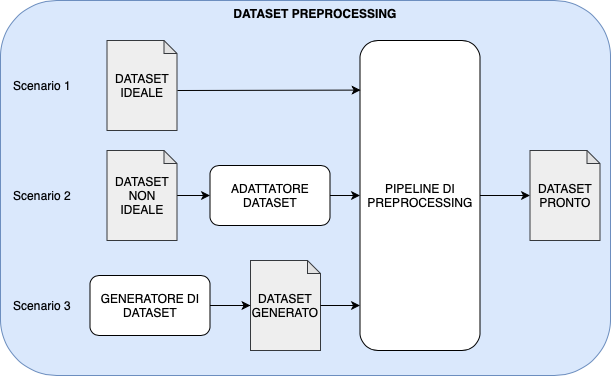
\includegraphics[scale=0.6]{images/preprocessingmodule.png}
    \caption{Primo nodo dell'architettura, dedicato al preprocessing dei dati, secondo i tre possibili scenari.}
    \label{preprocessmodule}
\end{figure}

\paragraph{Selezione dei modelli}
La fase di selezione dei modelli si occupa di individuare il modello ideale tenendo presente le considerazioni relative alla valutazione della capcità predittiva e alla bontà di generalizzazione dei modelli fatte nei Paragrafi~\ref{evaluation} e~\ref{generalization}.

Al fine di rendere computazionalmente più agevole l'esecuzione degli esperimenti si è optato per isolare ciascun nodo per permettere, ad ogni step, la scrittura in memoria persistente dell'output. Nel caso della model selection risulta particolarmente conveniente disporre di un dataset precedentemente elaborato su cui impostare la selezione dei modelli in quanto, innanzitutto potrebbe richiedere notevole tempo per terminare, e soprattutto lo stesso campione elaborato potrebbe essere utilizzato più volte.

I modelli ottimali vengono generati tramite la tecnica della cross validation annidata e, per ciascuna iterazione, viene fatta una \textit{grid search} per indagare quali siano i migliori modelli sulla base del validation error ottenuto.

Alla fine di questa operazione vengono ricavati, infatti, i modelli che si sono adattati meglio ai dati e fornita la relativa configurazione degli iperparametri.

\`E in questa fase che si colloca l'utilizzo di $\mu$-learn in quanto le configurazioni della grid search riguardano gli iperparametri di tale algoritmo.
I modelli selezionati vengono, dunque, serializzati per permettere il loro riutilizzo in un secondo momento; più precisamente, questo avviene nel terzo nodo di visualizzazione dei dati in cui si vuole valutare il loro comportamento.

In Figura~\ref{selectionmodel} viene mostrata la rappresentazione del funzionamento sopra descritto.
\begin{figure}
    \centering
    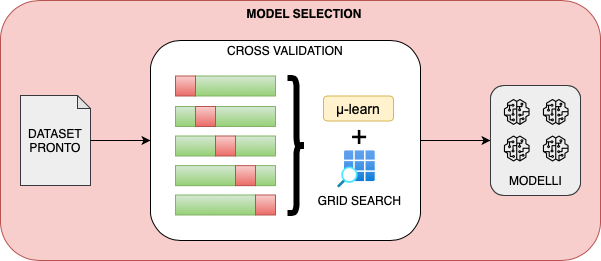
\includegraphics[scale=0.6]{images/modelselectionmodule.png}
    \caption{Secondo nodo dell'architettura, dedicato alla selezione dei modelli.}
    \label{selectionmodel}
\end{figure}

\paragraph{Visualizzazione dei dati} 
Nella parte di visualizzazione dei dati, i modelli vengono deserializzati per poterli riutilizzare al fine di operare un'analisi descrittiva.
Tale analisi coinvolge principalmente i gradi di appartenenza approssimati dai modelli generati dal sistema, valutando la bontà delle predizioni da essi effettuate.

Il criterio con cui viene valutata la correttezza delle predizioni consiste nell'utilizzare le misure quantitative descritte nei Paragrafi~\ref{erroreclass} e~\ref{erroreregr}. Si sottolinea, inoltre, che in questa fase vengono effettuati dei confronti con una determinata \textit{baseline}, ovvero uno o più stimatori di riferimento le cui predizioni vengono valutate sugli stessi dati trattati da $\mu$-learn, per poter fornire un ulteriore metro di paragone. Come mostrato in Figura~\ref{datavisualization}, l'analisi può interagire nuovamente col dataset di partenza per poter visionare quelle osservazioni che causano incertezza nelle predizioni. Complessivamente, il terzo nodo è importante per poter estrarre maggior conoscenza dall'ambito preso in considerazione. Tutte le conclusioni tratte dall'analisi descrittiva, infatti, vengono riassunte in un report e, sulla base di esso, si può eventualmente decidere se ricominciare gli esperimenti.

\begin{figure}
    \centering
    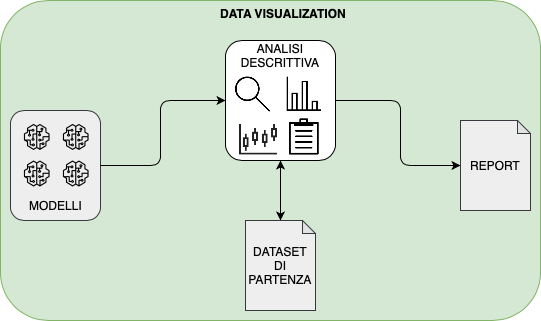
\includegraphics[scale=0.6]{images/datavisualizationmodule.png}
    \caption{Terzo nodo dell'architettura, dedicato alla visualizzazione dei dati.}
    \label{datavisualization}
\end{figure}

\subsection{Funzionamento del sistema}
In questo paragrafo si descrive come funziona il sistema nella sua complessità e come esso sia stato utilizzato per produrre dei risultati.
\begin{figure}[!ht]
    \centering
    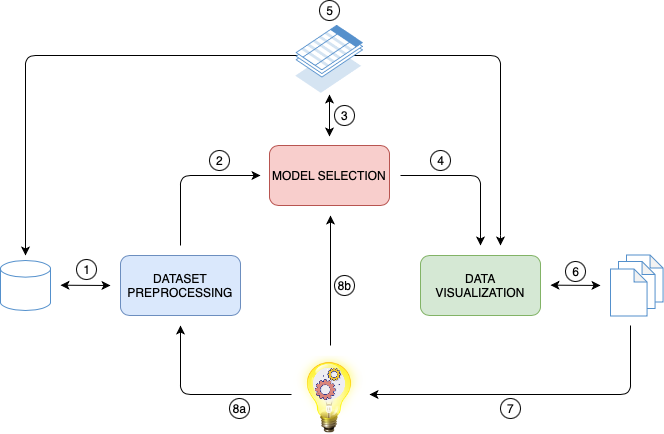
\includegraphics[scale=0.6]{images/cycle.png}
    \caption{Schema del flusso di comunicazione all'interno del sistema.}
    \label{cycle}
\end{figure}
In Figura~\ref{cycle} viene raffigurato il flusso di comunicazione all'interno del sistema, numerato passo per passo: 
\begin{enumerate}
    \item il processo ha inizio quando si dispone di un dataset, ottenuto in uno dei modi visti in precedenza, e viene così acquisito dal primo nodo per il preprocessing;
    \item  il nodo effettua il preprocessing del dataset e ne produce uno nuovo che viene opportunamente scritto su file per permettere la successiva lettura da parte del nodo di model selection;
    \item i modelli predittivi ottimali sono stati trovati, serializzati e il sistema aggiorna la storia degli esperimenti, documentata in un registro dedicato. Lo scopo del registro è catalogare i modelli e i loro dati associati tramite l'informazione di data e ora;
    \item i modelli vengono deserializzati e usati per l'analisi descrittiva delle predizioni;
    \item tramite il registro, il sistema è in grado di risalire al dataset utilizzato per ottenere i relativi modelli e, dunque, completare l'analisi;
    \item il modulo per la visualizzazione dei dati fornisce un report che viene aggiunto a quelli associati agli altri esperimenti;
    \item il report permette di analizzare il comportamento dei modelli e individuare delle possibili configurazioni da testare per i nuovi esperimenti;
    \item se si desira fare nuovi esperimenti
    
    a) ripartendo dal preprocessing dei dati, è necessario ricominciare l'esperimento dall'inizio, andando a modificare i parametri in questione;
    
    b) modificando il modo in cui viene fatta la grid search, si regolano i relativi valori a partire dalla model selection.
\end{enumerate}

\section{Tipi di predittore considerati}\label{predictors}
Le considerazioni fatte nei Paragrafi~\ref{erroreclass} e~\ref{erroreregr} portano a domandarsi quale tipo di predittore sia il caso di considerare per il problema delle fake news.

Sono state esplorate due possibilità: la pura induzione della funzione di appartenenza e un classificatore binario derivato da tale induzione.
Siano $\lambda$ e $\omega$ i due predittori appena presentati, si definisce il primo predittore come
\begin{equation}
    \lambda: \mathbb{R}^h \rightarrow [0,1]
\end{equation}
dove $h$ è il numero di feature; sia $x$ una generica osservazione del dataset, il secondo predittore $w: \mathbb R^h \rightarrow \{ 0, 1 \}$ è definito come
\begin{equation}
    \omega(x) = \begin{cases} 1 & \mbox{se } \lambda(x) \geq 0.5, \\ 0 & \mbox{altrimenti.} \end{cases}
\end{equation}
Ne consegue che per $\lambda$ risultano più appropriate le misure di MSE e RMSE, mentre per $\omega$ sono state scelte le metriche di Precision, Recall e F1\footnote{In realtà si tratta di una versione leggermente modificata: si tratta di calcolare le misure di Precision, Recall e F1 pesando il numero di veri positivi e falsi positivi con $\mu$ e il numero di falsi negativi per $1-\mu$.}.

\chapter{Implementazione}
\label{Capitolo 3}
\onehalfspacing
Questo capitolo tratta l'implementazione della soluzione proposta nel capitolo precedente. Nel Paragrafo~\ref{datasethandle} si descrive la parte inerente alle modalità con cui si gestiscono i vari scenari relativi al tipo di dataset che si ha a disposizione.

All'interno del Paragrafo~\ref{pp} viene illustrata la pipeline di preprocessing, soffermandosi su ognuno degli step che la compongono; il Paragrafo~\ref{modelselection}, invece, descrive come è stata implementata la parte di model selection tramite la grid search.
Infine, nel Paragrafo~\ref{datavisualizationimpl} viene descritta la fase di visualizzazione dei dati.

\section{Gestione dei dataset}\label{datasethandle}
Il sistema di apprendimento supervisionato proposto in questa tesi ha bisogno di molti esempi per affinare le predizioni, pertanto sono stati previsti più scenari al fine di massimizzare la mole di dati destinata all'addestramento. Principalmente, le vie percorse sono state due: utilizzare un dataset acquisito da terzi e generarlo.
Nel primo caso servizi come \textit{Kaggle} hanno facilitato l'individuazione di dataset interessanti, mentre nel secondo è stato implementato un modulo adibito alla generazione artificiale di documenti testuali.

\subsection{Adattatore di dataset}\label{adapter}
Per gestire la diversità della forma dei dati, si è deciso di fissare un formato standard e, in base ad esso, adattare o meno il dataset a disposizione in modo che rispetti tale convenzione. L'obiettivo è facilitare l'esecuzione di tutto il sistema su nuovi dati.
Il sistema descritto nel Paragrafo~\ref{sistema} assume, quindi, un dataframe di tre colonne: \textit{index}, \textit{text} e \textit{label}.

L'indice ha la finalità di preservare l'identificatore di ogni osservazione, questo torna particolarmente utile i) quando si vogliono analizzare specifiche notizie durante la fase di data visualization; ii) per mantenere il riferimento alla posizione originale delle notizie rimescolate durante lo step di shuffling nel preprocessing.

Il testo riguarda delle possibili sequenze di parole che, nell'ambito delle fake news, possono essere il corpo delle notizie, i titoli o, a seconda del dataset considerato, dei possibili tweet o post sui social media.

L'etichetta ha due forme possibili: un valore binario o un valore compreso nell'intervallo $[0,1]$ per il caso di dataset generati.

\subsection{Generatore di dataset}\label{generator}
Oltre a poter trattare osservazioni con etichette categorici relative a notizie che sono fake o meno, è possibile considerare anche dei dati etichettati con il grado di appartenenza. Un tipo di dataset così organizzato è più difficile da reperire; di conseguenza, al fine di produrre degli esperimenti più esaustivi, si è deciso di implementare un modulo per la generazione di dataset con il grado di appartenenza. Il modulo in questione si basa sulla tecnica di \textit{Latent Dirichlet Allocation} (\textit{LDA} \cite{20}) per la creazione di documenti testuali come misture di parole appartenenti a topic diversi. 
Si denoti, quindi, $t_1$ il topic delle notizie vere e $t_2$ quello delle notizie fake; ciascun topic è rappresentato da un insieme di parole $P_i$ che lo caratterizza. Per semplicità, è stato considerato prima il caso di $P_1 \cap P_2 = \emptyset$ e poi quello dell'intersezione non vuota.

La tecnica prevede la generazione di $m$ documenti composti da $n$ parole estratte dai topic nel modo seguente: 
\begin{itemize}
    \item si fissa l'insieme $P_2$, rappresentativo del topic $t_2$ delle fake news;
    \item si definisce, quindi, grado di appartenenza ``atteso'' dell'$i$-esimo documento la probabilità $\mu_i$ di successo di una distribuzione bernoulliana che una parola $p_j \in P_2$ venga inserita nel documento, con $i=1, ..., m$ e $j=1, ..., n$;
    \item si indicano con $B$ e $Z$ due variabili casuali che seguono rispettivamente la distribuzione bernoulliana e la distribuzione di Zipf \cite{34};
    \item si fissa un'arbitraria distribuzione di probabilità $d$;
    \item si esegue l'Algoritmo~\ref{lda}.
\end{itemize}  

\begin{algorithm}
\caption{procedura del \texttt{generatore di dataset}}
\label{lda}
\hspace*{\algorithmicindent} \textbf{Procedure} generator($m$, $n$, $d$, $P$)
\newline
\hspace*{\algorithmicindent} \textbf{Input}: $m$ è il numero di documenti, $n$ il numero di parole per ogni documento, $d$ è la distribuzione arbitraria, $P$ è la lista che contiene $P_1$ e $P_2$: gli insiemi di parole che rappresentano i due topic
\newline
\hspace*{\algorithmicindent} \textbf{Output}: $m$ documenti testuali artificiali
\begin{algorithmic}[1]
\STATE documents = [ ]
\FOR{$i$ in $1, ..., m$}
\STATE $\mu_i$ = extraction($d$)
\STATE document = [ ]
\STATE document.membership = $\mu_i$
\FOR{$j$ in $1, ..., n$}
\STATE $B$ = extraction(bernoulli, probability = $\mu_i$)
\STATE $Z$ = extraction(zipf)
\STATE word = $P$.index($B, Z$)
\STATE document.add(word)
\ENDFOR
\STATE documents.add(document)
\ENDFOR
\RETURN documents
\end{algorithmic}
\end{algorithm}
In pratica, si tratta di un processo non deterministico di estrazione delle parole, in cui la variabile $Z$ indica la parola estratta e $B$ è la variabile casuale bernoulliana che determina il topic selezionato in base alla probabilità di successo $\mu_i$. Nel caso di due topic si hanno due valori possibili: 0 per il topic delle notizie vere e 1 per le fake news, allora si definisce di ``successo'' l'evento $B=1$ con probabilità $\mu_i$ e l'evento di ``insuccesso'' $B=0$ con probabilità $1-\mu_i$, o equivalentemente
\begin{equation}
    \mathsf{P}(p_j \in P_2) = \mu_i,
\end{equation}
\begin{equation}
    \mathsf{P}(p_j \in P_1) = 1 - \mu_i.
\end{equation}
L'obiettivo del generatore è valutare la capacità predittiva di $\mu$-learn e capire la potenzialità di questo approccio nell'avvicinarsi al grado di appartenenza atteso.

\section{Pipeline di preprocessing}\label{pp}
Per la fase di preprocessing è stata predisposta una pipeline, ovvero un insieme di operazioni eseguite consecutivamente.

La sequenza di operazioni viene configurata al momento dell'esecuzione tramite un'opportuna parametrizzazione degli step della pipeline.

Ogni operazione segue il pattern di implementazione della libreria \textit{scikit-learn} che prevede di separare le procedure di \textit{fit} e \textit{transform}: esse definiscono rispettivamente la parte di apprendimento dei dati, quando richiesta, e quella di effettiva trasformazione dell'input in un output elaborato.
Adottare questa convenzione rappresenta un vantaggio per poter accedere alle funzioni della suddetta libreria parametrizzando le operazioni.
Inoltre, il codice organizzato in questa maniera si presta bene a future estensioni e favorisce la sua manutenibilità poiché rispetta il criterio della \textit{Separation of Concerns}, concetto cardine nell'ambito dell'Ingegneria del software \cite{32}.

Quella che segue è la lista dei parametri della pipeline che al momento della configurazione è possibile attivare a seconda delle esigenze:
\begin{itemize}
    \item lowercase,
    \item rimozione dei duplicati,
    \item lemmatizzazione,
    \item tokenizzazione,
    \item rimozione del rumore,
    \item stemming,
    \item rimozione delle stop word,
    \item word2vec,
    \item aggregazione,
    \item doc2vec.
\end{itemize}
Addizionalmente si considera anche uno step di shuffling che fa una permutazione delle righe e uno finale di standardizzazione che porta i valori delle feature in un'unica scala.

In generale, le operazioni della pipeline non sono tutte compatibili, al contrario, alcune sono tra di loro esclusive, come Word2Vec e Doc2Vec, oppure la lemmatizzazione e lo stemming.
Inoltre, l'ordine con cui esse vengono applicate è determinante per la rielaborazione del testo: è più semplice rimuovere il rumore analizzando i token piuttosto che le stringhe di intere frasi, ecco perché la tokenizzazione avviene tipicamente nei primi step della pipeline. Un altro esempio è quello dell'aggregazione che, come visto nei Paragrafi~\ref{w2v} e~\ref{d2v}, è necessaria solo in caso di utilizzo di Word2Vec.
\begin{figure}
    \centering
    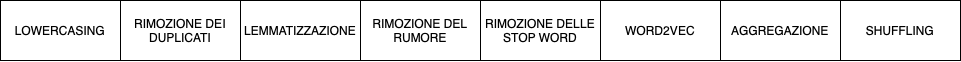
\includegraphics[scale=0.4]{images/pipeline.png}
    \caption{Esempio di configurazione di una pipeline di preprocessing.}
    \label{pipeline}
\end{figure}
In Figura~\ref{pipeline} viene mostrato un esempio di pipeline che è stata frequentemente utilizzata durante gli esperimenti. Si noti come in questo tipo di configurazione non sia necessario includere lo step di tokenizzazione in quanto la lemmatizzazione prevede una suddivisione in token che garantisce lo stesso risultato.
Nei paragrafi successivi si descrivono brevemente i possibili passi della pipeline.

\paragraph{Lowercasing}
Il \textit{lowercasing} è una tecnica che consiste nel trasformare una stringa di testo in una stringa composta unicamente da caratteri minuscoli.
\\
\\
\textbf{Input}: dataframe di stringhe:
\begin{center}
    \begin{tabular}{|c|c|}
    \hline
    \textbf{index} & \textbf{text} \\
    \hline
         0 & `\textit{This is a sentence. Lowercasing is going to do its job.}'\\
         1 & `\textit{This is another sentence.}'\\
    \hline
    \end{tabular}
\end{center}
\textbf{Output}: dataframe di stringhe:
\begin{center}
    \begin{tabular}{|c|c|}
    \hline
    \textbf{index} & \textbf{text} \\
    \hline
         0 & `\textit{this is a sentence. lowercasing is going to do its job.}'\\
         1 & `\textit{this is another sentence.}'\\
    \hline
    \end{tabular}
\end{center}

\paragraph{Rimozione dei duplicati}
In questo step vengono rimossi i duplicati presenti nel dataset, intesi come le osservazioni ripetute nel dataset.
\\
\\
\textbf{Input}: dataframe di stringhe:
\begin{center}
    \begin{tabular}{|c|c|}
    \hline
    \textbf{index} & \textbf{text} \\
    \hline
         0 & `\textit{This is a duplicate sentence.}'\\
         1 & `\textit{This is a duplicate sentence.}'\\
         2 & `\textit{This is another sentence.}'\\
    \hline
    \end{tabular}
\end{center}
\textbf{Output}: dataframe di stringhe:
\begin{center}
    \begin{tabular}{|c|c|}
    \hline
    \textbf{index} & \textbf{text} \\
    \hline
         0 & `\textit{This is a duplicate sentence.}'\\
         1 & `\textit{This is another sentence.}'\\
    \hline
    \end{tabular}
\end{center}

\paragraph{Lemmatizzazione}
La \textit{lemmatizzazione} è la tecnica che ricava da una frase i lemmi che la compongono sulla base della morfologia delle parole.
Questo step include implicitamente la divisione in token.
Si osservi, inoltre, che nel caso di pronomi la lemmatizzazione produce una generica stringa \texttt{-PRON-} in quanto morfologicamente non esiste una base.
\\
\\
\textbf{Input}: dataframe di stringhe:
\begin{center}
    \begin{tabular}{|c|c|}
    \hline
    \textbf{index} & \textbf{text} \\
    \hline
         0 & `\textit{this is a sentence that is going to be split.}'\\
         1 & `\textit{here another sentence which confirms it.}'\\
    \hline
    \end{tabular}
\end{center}
\textbf{Output}: dataframe di liste di stringhe:
\begin{center}
    \begin{tabular}{|c|c|}
    \hline
    \textbf{index} & \textbf{text} \\
    \hline
         0 & [\textit{`this', `be', `a', `sentence', `that', `be', `go', `to', `be', `split', `.'}]\\
         1 & [\textit{`here', `another', `sentence', `which', `confirm', `-PRON-', `.'}]\\
    \hline
    \end{tabular}
\end{center}

\paragraph{Tokenizzazione}
La \textit{tokenizzazione} consiste nella pura suddivisione delle frasi in token. Per token si intende un'istanza di una sequenza di caratteri raggrupati in modo da formare una semantica, tipicamente si tratta di parole.
\\
\\
\textbf{Input}: dataframe di stringhe:
\begin{center}
    \begin{tabular}{|c|c|}
    \hline
    \textbf{index} & \textbf{text} \\
    \hline
         0 & `\textit{This is a sentence that is going to be split.}'\\
         1 & `\textit{Here there is another sentence which confirms it.}'\\
    \hline
    \end{tabular}
\end{center}
\textbf{Output}: dataframe di liste di stringhe:
\begin{center}
    \begin{tabular}{|c|c|}
    \hline
    \textbf{index} & \textbf{text} \\
    \hline
         0 & [\textit{`This', `is', `a', `sentence', `that', `is', `going', `to', `be', `split', `.'}]\\
         1 & [\textit{`Here', `there', `is', `another', `sentence', `which', `confirms', `it', `.'}]\\
    \hline
    \end{tabular}
\end{center}

\paragraph{Rimozione del rumore}
La \textit{rimozione del rumore} è, a sua volta, scomponibile in molteplici passaggi, ciascuno delegato alla rimozione di uno specifico tipo di rumore.
In tal senso, sono stati implementate le rimozioni di URL, emoji, punteggiatura, numeri, parole contenenti numeri, parole duplicate, e osservazioni vuote nel dataset. 
\\
\\
\textbf{Input}: dataframe di liste di stringhe:
\begin{center}
    \begin{tabular}{|c|c|}
    \hline
    \textbf{index} & \textbf{text} \\
    \hline
         0 & [\textit{`This', `is', `www.unimi.it', `\smiley{}'}, `,', `my', `number', `is', `928792', `.']\\
         1 & [\textit{ }] \\
         2 & [\textit{`My', `username', `is', `fire95'}] \\
    \hline
    \end{tabular}
\end{center}
\textbf{Output}: dataframe di liste di stringhe:
\begin{center}
    \begin{tabular}{|c|c|}
    \hline
    \textbf{index} & \textbf{text} \\
    \hline
         0 & [\textit{`This', `is', `my', `number'}]\\
         1 & [\textit{`My', `username', `is'}] \\
    \hline
    \end{tabular}
\end{center}

\paragraph{Stemming}
Lo \textit{stemming} ha l'obiettivo di rimuovere suffissi e prefissi per individuare la radice delle parole.
\\
\\
\textbf{Input}: dataframe di liste di stringhe:
\begin{center}
    \begin{tabular}{|c|c|}
    \hline
    \textbf{index} & \textbf{text} \\
    \hline
         0 & [\textit{`this', `is', `a', `sentence', `that', `is', `going', `to', `be', `split', `.'}]\\
         1 & [\textit{`here', `there', `is', `another', `sentence', `which', `confirms', `it', `.'}]\\
    \hline
    \end{tabular}
\end{center}
\textbf{Output}: dataframe di liste di stringhe:
\begin{center}
    \begin{tabular}{|c|c|}
    \hline
    \textbf{index} & \textbf{text} \\
    \hline
         0 & [\textit{`thi', `is', `a', `sentenc', `that', `is', `go', `to', `be', `split', `.'}]\\
         1 & [\textit{`here', `there', `is', `anoth', `sentenc', `which', `confirm', `it', `.'}]\\
    \hline
    \end{tabular}
\end{center}

\paragraph{Rimozione delle stop word}
Come accennato nel Capitolo~\ref{Capitolo 1}, si può scegliere di rimuovere le \textit{stop word}, parole molto frequenti all'interno di un documento ma che poco aggiungono alla semantica del testo.
\\
\\
\textbf{Input}: dataframe di liste di stringhe:
\begin{center}
    \begin{tabular}{|c|c|}
    \hline
    \textbf{index} & \textbf{text} \\
    \hline
         0 & [\textit{`this', `is', `a', `sentence', `with', `stop', `words'}]\\
         1 & [\textit{`here', `there', `is', `another', `interesting', `case'}]\\
    \hline
    \end{tabular}
\end{center}
\textbf{Output}: dataframe di liste di stringhe:
\begin{center}
    \begin{tabular}{|c|c|}
    \hline
    \textbf{index} & \textbf{text} \\
    \hline
         0 & [\textit{`sentence', `stop', `word'}]\\
         1 & [\textit{`interesting', `case'}]\\
    \hline
    \end{tabular}
\end{center}

\paragraph{Word2Vec}
\textit{Word2Vec} è la prima delle due tecniche di embedding citate in questa tesi che converte ogni parola in un vettore di feature numeriche; l'esempio considera 96 feature.
\\
\\
\textbf{Input}: dataframe di liste di stringhe:
\begin{center}
    \begin{tabular}{|c|c|}
    \hline
    \textbf{index} & \textbf{text} \\
    \hline
         0 & [\textit{`thi', `sentenc', `split'}]\\
         1 & [\textit{`anoth', `sentenc', `confirm'}]\\
    \hline
    \end{tabular}
\end{center}
\textbf{Output}: dataframe di liste di liste di valori float:
\begin{center}
    \begin{tabular}{|c|c|}
    \hline
    \textbf{index} & \textbf{text} \\
    \hline
         0 & [[1.12, ..., -3.6],[-1.83, ..., -2.20],[-0.96, ..., -1.04]] (3 liste di 96 elementi) \\
         1 & [[-0.32, ..., -1.96],[-1.83, ..., -2.20],[0.20, ..., -2.60]] (3 liste di 96 elementi)\\
    \hline
    \end{tabular}
\end{center}

\paragraph{Aggregazione}
La fase di \textit{aggregazione} è necessaria nel caso si utilizzi Word2Vec, poiché l'obiettivo finale è ottenere nuovamente un dataframe di vettori. In questo esempio si mostra l'aggregazione tramite la media dei vettori.
\\
\\
\textbf{Input}: dataframe di liste di liste di valori float:
\begin{center}
    \begin{tabular}{|c|c|}
    \hline
    \textbf{index} & \textbf{text} \\
    \hline
         0 & [[1.12, ..., -3.60],[-1.83, ..., -2.20],[-0.96, ..., -1.04]] (3 liste di 96 elementi) \\
         1 & [[-0.32, ..., -1.96],[-1.83, ..., -2.20],[0.20, ..., -2.60]] (3 liste di 96 elementi) \\
    \hline
    \end{tabular}
\end{center}
\textbf{Output}: dataframe di liste di valori float:
\begin{center}
    \begin{tabular}{|c|c|}
    \hline
    \textbf{index} & \textbf{text} \\
    \hline
         0 & [-0.81, -0.63, ..., -2.24] (96 elementi) \\
         1 & [-0.88, -1.22, ..., -2.22] (96 elementi) \\
    \hline
    \end{tabular}
\end{center}

\paragraph{Doc2Vec}
\textit{Doc2Vec} è una soluzione alternativa di embedding per convertire direttamente le frasi in vettori; essa non necessita, infatti, di una fase di aggregazione ma richiede come input un dataframe di stringhe.
L'esempio considera un modello di 20 feature 
\\
\\
\textbf{Input}: dataframe di stringhe:
\begin{center}
    \begin{tabular}{|c|c|}
    \hline
    \textbf{index} & \textbf{text} \\
    \hline
         0 & \textit{`thi sentenc split'}\\
         1 & \textit{`anoth sentenc confirm'}\\
    \hline
    \end{tabular}
\end{center}
\textbf{Output}: dataframe di liste di float:
\begin{center}
    \begin{tabular}{|c|c|}
    \hline
         0 & [0.02, 0.03, ..., 0.04] (20 elementi) \\
         1 & [-0.01, -0.03, ..., 0.03] (20 elementi) \\
    \hline
    \end{tabular}
\end{center}

\paragraph{Shuffling}
Fare lo \textit{shuffling} dei dati significa effettuare una permutazione delle righe per assicurarsi che il dataset non segua uno specifico ordine. Quando questo accade, infatti, il partizionamento in training, validation e test set (o in generiche fold) rischia di essere fortemente influenzato dal modo in cui i dati sono collocati e di determinare degli insiemi poco rappresentativi del problema che si vuole modellare: si supponga, ad esempio, di voler generare un classificatore di un set di animali e che i dati siano organizzati in ordine alfabetico. Nel dataset, quindi, saranno presenti prima tutti i cani, poi tutti i gatti, poi i leoni, e via discorrendo. Nel contesto della cross validation, ad esempio, rimescolare i dati significa evitare che si creino fold composte interamente, o quasi, solo da cani, solo da gatti o leoni. Questo fenomeno da evitare prende il nome di \textit{bias dei dati}.
\\
\\
\textbf{Input}: dataframe preprocessato:
\begin{center}
    \begin{tabular}{|c|c|c|}
    \hline
    \textbf{index} & \textbf{text} & \textbf{label} \\
    \hline
         0 & [0.02, 0.03, ..., 0.04] (20 elementi) & 1 \\
         1 & [-0.01, -0.03, ..., 0.03] (20 elementi) & 1 \\
         2 & [0.04, 0.01, ..., 0.91] (20 elementi) & 0 \\
         3 & [-0.07, 0.31, ..., 0.02] (20 elementi) & 0 \\
    \hline
    \end{tabular}
\end{center}
\textbf{Output}: dataframe preprocessato e rimescolato:
\begin{center}
    \begin{tabular}{|c|c|c|}
    \hline
    \textbf{index} & \textbf{text} & \textbf{label} \\
    \hline
        3 & [-0.07, 0.31, ..., 0.02] (20 elementi) & 0 \\
        0 & [0.02, 0.03, ..., 0.04] (20 elementi) & 1 \\
        2 & [0.04, 0.01, ..., 0.91] (20 elementi) & 0 \\
        1 & [-0.01, -0.03, ..., 0.03] (20 elementi) & 1 \\
    \hline
    \end{tabular}
\end{center}

\paragraph{Standardizzazione}\label{standardization}
È presente, inoltre, un passaggio finale della pipeline che riguarda la standardizzazione dei dati. In letteratura sono presenti molteplici opzioni, ad esempio la trasformazione \textit{Min-Max} oppure quella basata sul \textit{range interquartile}. In questo caso è stata scelta la tecnica che mira a calcolare i punti \textit{z-score}: si applica ad ogni osservazione la seguente trasformazione:
\begin{equation}
    z_i = \frac{x_i - \mu}{\sigma}
\end{equation}
con $x_i$ l'$i$-esima osservazione e $\mu$ e $\sigma$, rispettivamente la media e la deviazione standard della distribuzione delle feature; si ottiene, quindi, una distribuzione standardizzata centrata nell'origine e deviazione standard pari a 1.

\section{Selezione dei modelli}\label{modelselection}
Nel processo di apprendimento di un task predittivo vengono generati numerosi modelli; per questa ragione diventa cruciale utilizzare un criterio di selezione di tali modelli come la grid search per ricavare i migliori risultati possibili.

\subsection{Grid search}\label{gs}
La grid search è una tecnica di ricerca del modello migliore che, sostanzialmente, automatizza il processo di tuning.

Il termine grid deriva dal fatto che si preimposta una griglia di valori per tutti gli iperparametri di cui si desidera fare il tuning.

Un esempio di griglia viene mostrato in Tabella~\ref{grid}: in questo caso è stato fissato il tipo di fuzzificatore, il tipo di kernel e il tipo di solver, mentre è stato previsto un intervallo di dieci ordini di grandezza per $\sigma$, parametro del kernel gaussiano, e per $C$.
\begin{table}
\centering
 \begin{tabular}{|c|c|c|c|c|} 
 \hline
\textbf{fuzzificatore} & \textbf{kernel} & \textbf{solver} & $\bm{\sigma}$ & \textit{\textbf{C}} 
\\ [0.5ex] 
 \thickhline
 lineare & gaussiano & gurobi & logspace(-5, 5, 11) & logspace(-5, 5, 11) \\ 
 \hline
\end{tabular}
\caption{Esempio di griglia di iperparametri.}
\label{grid}
\end{table}
Chiaramente, più ampio è il set di valori da ottimizzare, più computazionalmente costosa diventa l'esecuzione dell'algoritmo, in quanto necessita di reiterare ulteriormente il processo. In questo senso, l'esempio mostra anche l'evenienza in cui alcuni valori vengono fissati per favorire la ricerca di quelli ottimali per altri parametri, alleggerendo, dunque, il carico computazionale.

\paragraph{K-fold cross validation}
Lo stratagemma utilizzato da questa tecnica consiste nel dividere il dataset $S$ in $k$ partizioni $S_1, S_2, ..., S_k$, dette fold, tali che:
\begin{equation}
     S = \bigcup\limits_{i=1}^{k} S_{i},
\end{equation}
\begin{equation}
    S_i \cap S_j = \emptyset \ \ \forall i \neq j.
\end{equation}
Si denota con $S^{(i)} \equiv S \setminus S_i$ la parte per l'addestramento e $S_i$ la parte per la validazione, come illustrato in Figura~\ref{cv}.
Per completezza, nell'Algoritmo~\ref{kfold} vengono delineati i passi chiave della procedura: si fa un partizionamento in $k$ fold\footnote{Il partizionamento tipicamente tiene conto della rappresentatività delle fold ottenute: in \textit{Scikit-learn} esistono delle funzioni come \textit{StratifiedKFold} che permettono di operare una suddivisione tale che le fold abbiano un rapporto bilanciato delle occorrenze dei valori delle etichette.}, organizzandole in insiemi per il training e per il test, come visto sopra, e per ogni iterazione si genera un modello che viene valutato tramite delle metriche.
\begin{figure}
    \centering
    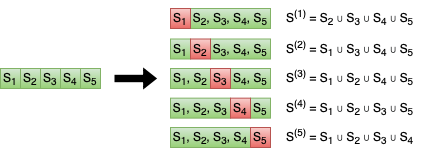
\includegraphics[scale=0.83]{images/cv.png}
    \caption{Schematizzazione del processo di cross validation: in rosso la parte per la validation e in verde la parte per il training.}
    \label{cv}
\end{figure}
\begin{algorithm}
\caption{\texttt{k-fold cross validation}}
\label{kfold}
\hspace*{\algorithmicindent} \textbf{Procedure} cv($S$, $k$)
\newline
\hspace*{\algorithmicindent} \textbf{Input}: $S$ è il dataset, $k$ il numero di fold
\newline
\hspace*{\algorithmicindent} \textbf{Output}: $k$ modelli
\begin{algorithmic}[1]
\STATE $S_1, S_2, ..., S_k$ = partitioning($S$, $k$)
\FOR{$S_i$ in $S_1, S_2, ..., S_k$}
\STATE test = $S_i$
\STATE train = $S \setminus S_i$
\STATE model = mulearn.fit(train)
\STATE predictions = model.predict(test)
\STATE evaluation = model.evaluate(predictions)
\STATE models.add(model)
\STATE evaluations.add(evaluation)
\ENDFOR
\RETURN models, evaluations
\end{algorithmic}
\end{algorithm}
Per combinare i vantaggi della cross validation con quelli della grid search è stata implementata quella che viene definita \textit{cross validation annidata}: si opera una cross validation esterna per prevenire l'overfitting e poi, per ciascuna fold, si fa una cross validation interna che ha l'obiettivo di testare tutte le combinazioni indicate nella griglia e selezionare i modelli che hanno ottenuto i risultati migliori.

La procedura descritta nell'Algoritmo~\ref{kfold} viene, pertanto, estesa, come mostrato nell'Algoritmo~\ref{nested}.
\begin{algorithm}
\caption{\texttt{cross validation annidata}}
\label{nested}
\hspace*{\algorithmicindent} \textbf{Procedure} nested\_cv($S$, $k$, $l$, $gs$)
\newline
\hspace*{\algorithmicindent} \textbf{Input}: $S$ è il dataset, $k$ il numero di fold esterne, $l$ il numero di fold interne, $gs$ la griglia di valori
\newline
\hspace*{\algorithmicindent} \textbf{Output}: $k$ modelli ottimizzati
\begin{algorithmic}[1]
\STATE $S_1, S_2, ..., S_k$ = partitioning($S$, $k$)
\FOR{$S_i$ in $S_1, S_2, ..., S_k$}
\STATE test = $S_i$
\STATE train = $S \setminus S_i$
\STATE $D_1, D_2, ..., D_L$ = partitioning(train, $l$)
\FOR{$D_j$ in $D_1, D_2, ..., D_l$}
\STATE in\_validation = $D_j$
\STATE in\_train = train $\setminus D_j$
\STATE optimized\_model = $gs$.fit(in\_train)
\STATE in\_predictions = optimized\_model.predict(in\_test)
\ENDFOR
\STATE optimized\_model = optimized\_model.fit(train)
\STATE predictions = optimized\_model.predict(test)
\STATE evaluation = optimized\_model.evaluate(predictions) 
\STATE optimized\_models.add(optimized\_model)
\STATE evaluations.add(evaluation)
\ENDFOR
\RETURN optimized\_models, evaluations
\end{algorithmic}
\end{algorithm}

\section{Visualizzazione dei dati}\label{datavisualizationimpl}
La parte di visualizzazione dei dati è fondamentale per rappresentare i risultati degli esperimenti e, possibilmente, trarre delle considerazioni utili per migliorare il sistema. \`E stata, quindi, predisposta l'analisi descrittiva dei risultati che comprende:
\begin{itemize}
    \item la distribuzione delle predizioni dei modelli,
    \item la distribuzione delle etichette attese,
    \item il confronto con una baseline,
    \item il riepilogo delle misure di errore o accuratezza.
\end{itemize}
Da tale modulo sono stati ricavati diversi report durante lo svolgimento di questa tesi ed essi hanno consentito di individuare la direzione in cui far proseguire gli esperimenti.

Nel prossimo capitolo verranno presentati gli esperimenti realizzati e gli esiti che tale analisi descrittiva ha permesso di riassumere.

\chapter{Valutazione sperimentale}
\label{Capitolo 4}
\onehalfspacing
In quest'ultimo capitolo si illustra nel dettaglio la consistente parte di esperimenti che è stata condotta durante il lavoro documentato da questa tesi.

Nel Paragrafo~\ref{dataset} vengono presentati i dataset che sono stati presi in considerazione per la sperimentazione del sistema descritto nel Capitolo~\ref{Capitolo 3}. Successivamente, all'interno del Paragrafo~\ref{esperimenti} vengono mostrati i risultati finali che sono stati prodotti.

\section{Dataset}\label{dataset}
All'interno del Paragrafo~\ref{datasethandle} sono stati definiti i possibili scenari per i dati tramite i quali il sistema di apprendimento è stato allenato. Per quanto riguarda i dataset raccolti da terzi, sono state identificate le seguenti possibilità:
\begin{enumerate}
    \item \texttt{Fake and real news dataset} - 44898 osservazioni - 111 MB,
    \item \texttt{All the News 2.0} - 2.7 milioni di osservazioni - 9.2 GB,
    \item \texttt{ProfNER} - 10000 osservazioni - 13.6 MB.
\end{enumerate}
Il primo comprende un misto di notizie pubblicate su testate giornalistiche negli Stati Uniti e di tweet, il secondo è ricco di notizie e di saggi su 27 diverse pubblicazioni americane mentre il terzo include dei tweet in lingua spagnola.

Al fine di trovare un compromesso accettabile tra il numero di esperimenti e la capacità computazionale a disposizione è stato scelto il primo dataset.

\subsection{Fake and real news dataset}\label{fakenewsdataset}
\textit{Fake and real news dataset} è un dataset disponibile sulla piattaforma \textit{Kaggle} che raccoglie notizie e tweet, separandoli in ``fake'' e ``true'' news. Più precisamente sono presenti 23481 osservazioni per la parte di notizie false e 21417 per quelle annotate come vere, formando, quindi, un dataset approssimativamente bilanciato. 
Le osservazioni sono composte da informazioni inerenti al titolo della notizia, al corpo, all'argomento in essa contenuto e alla data di pubblicazione. Nelle Figure~\ref{fake_sample} e~\ref{true_sample} viene mostrato un esempio per ciascun dataframe.
\begin{figure}
    \centering
    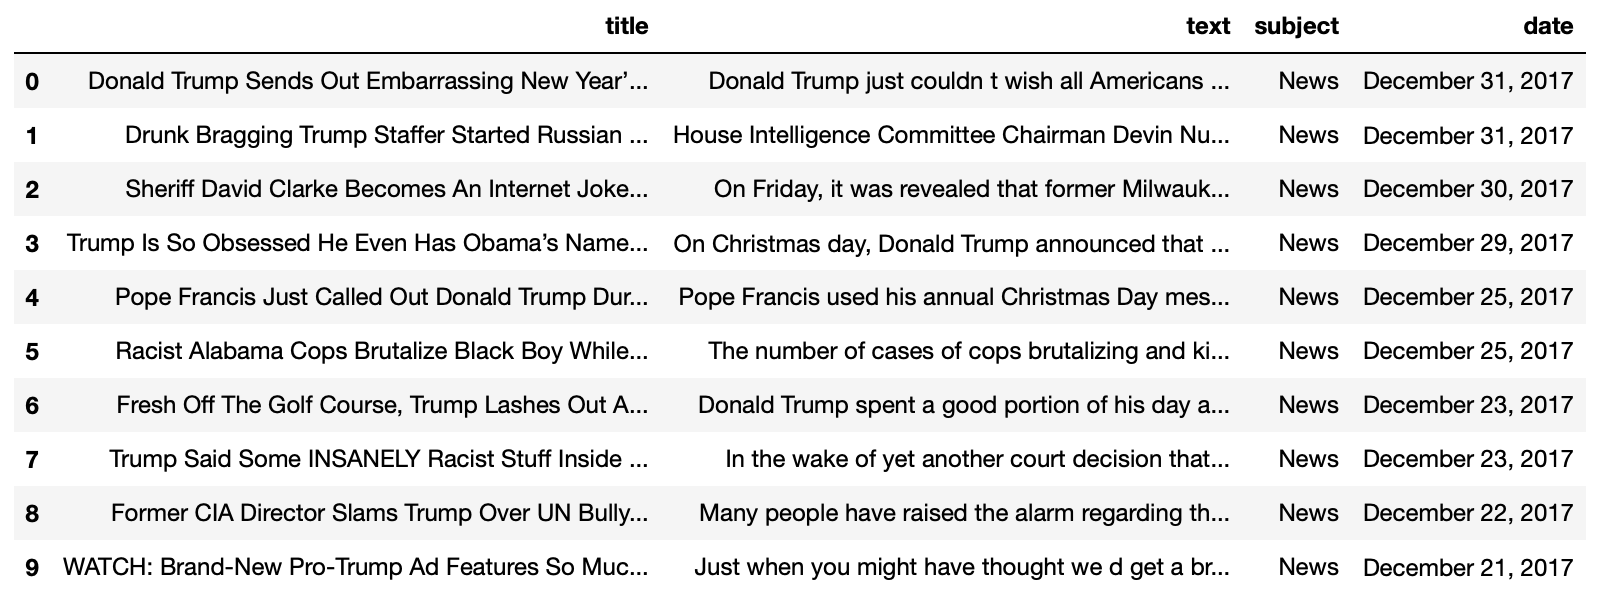
\includegraphics[scale=0.52]{images/fake_sample.png}
    \caption{Campione delle notizie del dataset etichettate come ``fake''.}
    \label{fake_sample}
\end{figure}
\begin{figure}
    \centering
    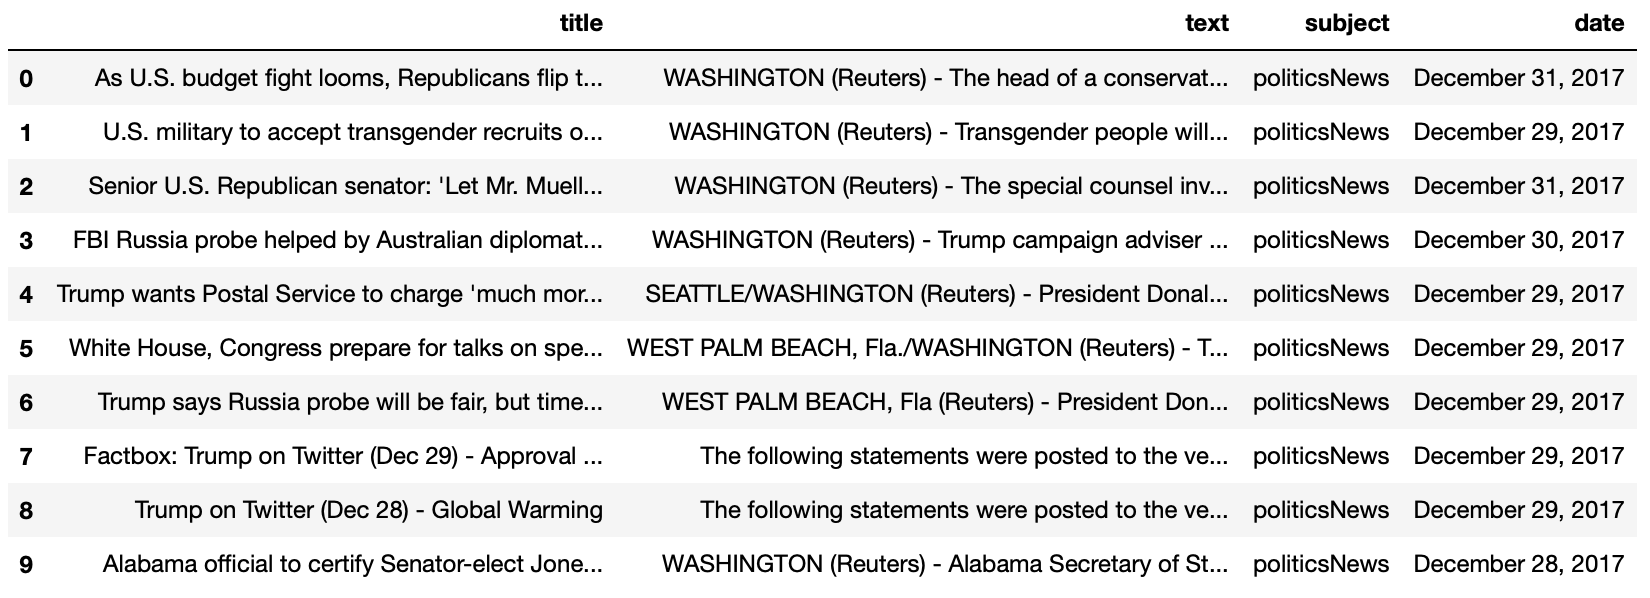
\includegraphics[scale=0.5]{images/true_sample.png}
    \caption{Campione delle notizie del dataset etichettate come ``vere''.}
    \label{true_sample}
\end{figure}
Si osserva la presenza di un'informazione temporale relativa al giorno di pubblicazione della notizia: questo rimanda alle premesse descritte nel Paragrafo~\ref{pp} che forniscono una motivazione convincente del perché, in casi come questi, la fase di shuffling sia necessaria al fine di prevenire un sovradattamento dovuto a un tale ordinamento.

La colonna relativa al titolo, per quanto rilevante, non è stata considerata ai fini dell'addestramento. La motivazione riguarda principalmente la presenza di tweet: in quel caso è difficile, infatti, parlare di ``titolo'', ed è tendenzialmente anche poco informativo (lo si evince facilmente dalla riga 8 del dataframe mostrato in Figura~\ref{true_sample}). Si presume, quindi, che tale informazione possa essere usata in congiunzione con altre come supporto.
Anche la colonna relativa all'argomento non è stata utilizzata, in quanto è stata rilevata una sostanziale differenza nella ricchezza di informazioni contenute per la parte di notizie vere rispetto a quelle fake, oltre che un'evidente inconsistenza degli argomenti identificati. Si conferma questo aspetto nella Tabella~\ref{subject}.
\begin{table}
\centering
 \begin{tabular}{|c|c|c|} 
 \hline 
 \textbf{argomento} & \textbf{fake news} & \textbf{true news}
\\ [0.5ex] 
 \thickhline
\texttt{News} & 38.54 \% & - \\
\texttt{politics} & 29.13 \% & -\\ 
\texttt{left-news} & 18.99 \% & -\\
\texttt{Government News} & 6.69 \% & -\\
\texttt{US\_News} & 3.33 \% & -\\
\texttt{Middle-east} & 3.31 \% & -\\
\texttt{politicsNews} & - & 52.63 \% \\
\texttt{worldnews} & - & 47.37 \% \\
 \hline
\end{tabular}
\caption{Frequenze relative degli argomenti.}
\label{subject}
\end{table}
Per questa parte di esperimenti si è deciso, quindi, di utilizzare unicamente l'informazione riguardante il corpo della notizia. 

Il suddetto dataset è stato elaborato tramite due pipeline di preprocessing: una per le fake news e una dedicata alle true news, ottenendo così dei vettori di feature a cui sono stati associati i valori binari delle etichette; infine, sono stati accorpati, rimescolati e standardizzati: un esempio di risultato è quello mostrato in Tabella~\ref{preprocesseddata}.
\begin{table}
\centering
 \begin{tabular}{|c|c|c|} 
 \hline 
 \textbf{index} & \textbf{text} & \textbf{label}
\\ [0.5ex] 
 \thickhline
22 & [0.34, 0.14, ..., 0.51] (96 elementi) & 1 \\
6 & [-0.45, -0.10, ..., 0.55] (96 elementi) & 0 \\ 
59 & [0.91, -0.92, ..., -1.14] (96 elementi) & 0\\
21 & [-0.86, 0.54, ..., 0.51] (96 elementi) & 1\\
12 & [0.11, 0.67, ..., -1.95] (96 elementi) & 0\\
132 & [0.83, -0.37, ..., 0.85] (96 elementi) & 1\\
 \hline
\end{tabular}
\caption{Esempio di dataset preprocessato.}
\label{preprocesseddata}
\end{table}

\subsection{Dataset generati}\label{generated_datasets}
Un approccio proposto per gli esperimenti è quello di utilizzare dei dataset generati tramite la tecnica descritta nel Paragrafo~\ref{generator}. Tale tecnica si basa sulla scelta di una distribuzione arbitraria $d$ che determina l'andamento dei valori del grado di appartenenza in funzione delle estrazioni di una variabile casuale. Al fine di fornire una panoramica esaustiva sono state scelte due distribuzioni: la distribuzione uniforme e la distribuzione beta.

\paragraph{Distribuzione uniforme}
Nella teoria delle Probabilità e in Statistica una delle distribuzioni più conosciute è sicuramente quella uniforme continua (Figura~\ref{uniforme}). Genericamente definita su un intervallo $[a,b]$, essa ha una funzione densità di probabilità
\begin{equation}
    f(x)= \begin{cases} \frac{1}{b-a} & \mbox{se } a\leq x \leq b, \\ 0 & \mbox{altrimenti.} \end{cases}
\end{equation}
Dal momento che il grado di appartenenza è compreso nell'intervallo $[0,1]$, anche la distribuzione uniforme selezionata è impostata su tale intervallo. 
\begin{figure}
    \centering
    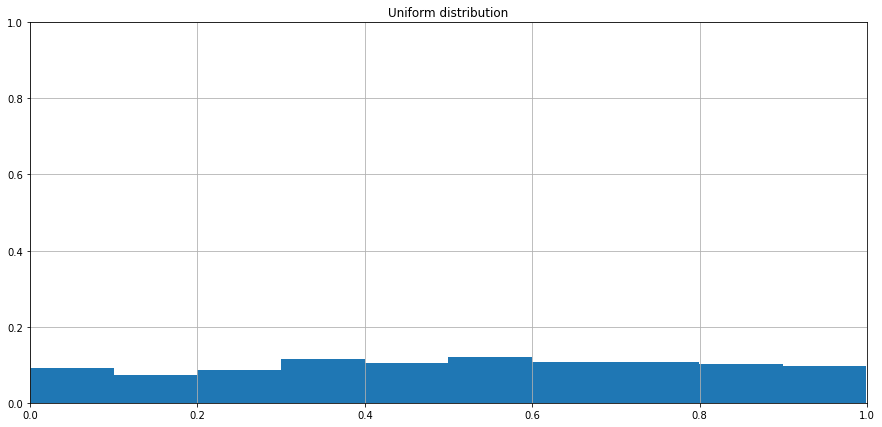
\includegraphics[scale=0.4]{images/uniform.png}
    \caption{Esempio di distribuzione approssimativamente uniforme.}
    \label{uniforme}
\end{figure}
\paragraph{Distribuzione beta}
L'altro tipo di distribuzione scelta è la distribuzione beta: a differenza di quella uniforme essa è specificatamente definita nell'intervallo $[0,1]$ e, dunque, adatta al contesto di generazione del grado di appartenenza. I parametri che ne regolano l'andamento sono due: $\alpha$ e $\beta$. La funzione densità di probabilità è:
\begin{equation}
    f(x)= \frac{x^{\alpha - 1}(1-x)^{\beta - 1}}{B(\alpha, \beta)}
\end{equation}
dove $B$ è la funzione
\begin{equation}
    B(\alpha, \beta) = \int_{0}^{1} x^{\alpha - 1}(1-x)^{\beta - 1} \,dx.
\end{equation}
Mediante questa distribuzione sono stati creati due scenari significativi:
\begin{enumerate}
    \item $\alpha = \beta = 5$ (Figura~\ref{beta5}),
    \item $\alpha = \beta = 0.5$ (Figura~\ref{beta05}).
\end{enumerate}
\begin{figure}
    \centering
    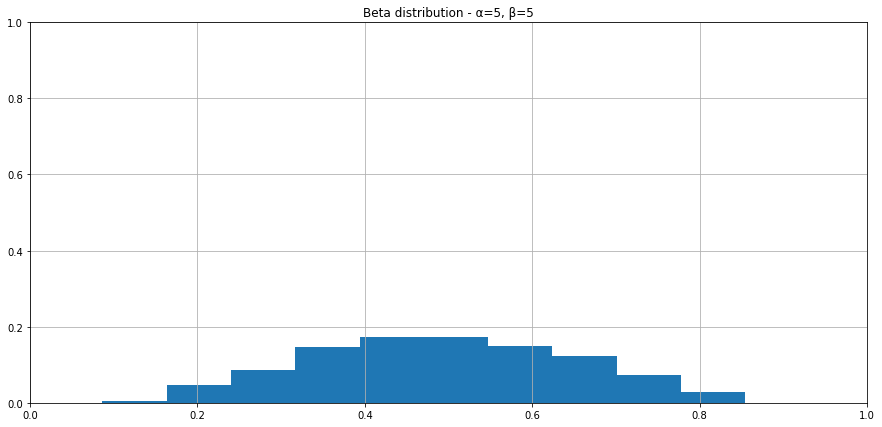
\includegraphics[scale=0.4]{images/beta5.png}
    \caption{Esempio di distribuzione approssimativamente beta, con parametri $\alpha = \beta = 5$.}
    \label{beta5}
\end{figure}
\begin{figure}
    \centering
    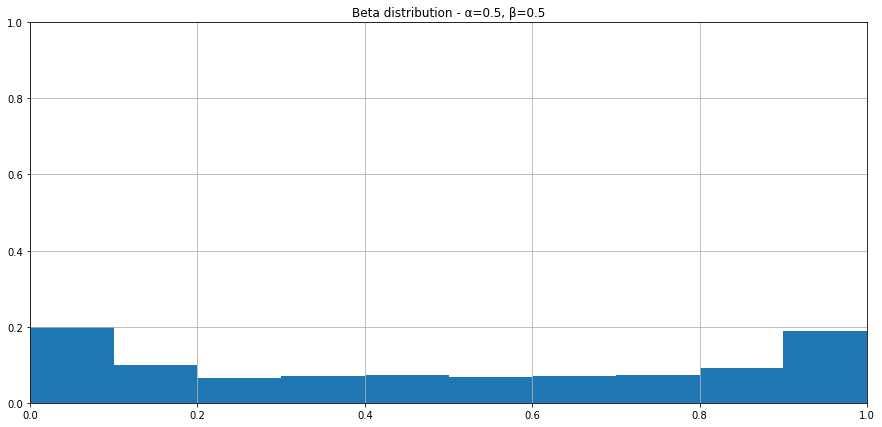
\includegraphics[scale=0.4]{images/beta05.png}
    \caption{Esempio di distribuzione approssimativamente beta, con parametri $\alpha = \beta = 0.5$.}
    \label{beta05}
\end{figure}
I tre scenari ottenuti consentono di testare la capacità dell'algoritmo di indurre la funzione di appartenenza fissando le distribuzioni viste finora. Il primo caso coinvolge gradi di appartenenza che hanno equa probabilità di occorrere, il secondo ha le sembianze di una distribuzione normale tagliata nell'intervallo $[0,1]$ e il terzo riproduce un fenomeno di polarizzazione delle occorrenze ai valori estremi dell'intervallo.

\subsubsection{Insiemi di parole} Il generatore di dataset, tramite le distribuzioni appena descritte, è in grado di creare dei documenti testuali sintetici a partire da insiemi di parole rappresentative di due topic.
Da un punto di vista lessicale, il problema non è banale e andrebbe approfondito determinando con cura l'insieme delle parole che contraddistinguono una notizia vera piuttosto che una fake.
Per questa parte di esperimenti sono state poste le basi per fare delle prove da una prospettiva puramente sintattica, con l'intenzione di fornire un punto di partenza per esperimenti futuri più accurati.

Si definiscono gli insiemi
\begin{center}
    $P_1$ = \texttt{\{arrogant, uptight, toothpaste, bottle, grass, show, ..., religion\}} (156 elementi)
\end{center}
\begin{center}
    $P_2$ = \texttt{\{ARROGANT, UPTIGHT, TOOTHPASTE, BOTTLE, GRASS, SHOW, ..., RELIGION\}} (156 elementi)
\end{center}
composti da termini inglesi randomici la cui semantica non viene considerata per le rilevazione delle fake news. Senza perdita di generalità si considera $P_1$ l'insieme rappresentativo del topic delle notizie vere e $P_2$ l'insieme associato alle fake news.

\paragraph{Insiemi disgiunti}
Dal momento che $P_1$ è completamente lowercase e $P_2$ uppercase, allora sintatticamente si ha che $P_1$ $\cap$ $P_2 = \emptyset$. Si parla, quindi, di insiemi disgiunti e la generazione di dataset avviene a partire da questi due insiemi. In Tabella~\ref{generationexample} viene riportato un esempio di generazione di documenti testuali al variare del grado di appartenenza. In questo caso è stato fissato come evento di successo il fatto che la parola generata appartenga all'insieme $P_2$; di conseguenza, all'aumentare di $\mu_i$ si osserva una crescente componente di parole maiuscole all'interno del documento generato.
\begin{table}
\centering
\begin{adjustbox}{max width=\textwidth}
 \begin{tabular}{|c|c|c|} 
 \hline
\textbf{id} & \textbf{esempio di testo ottenuto (1000 parole)} & $\bm{\mu_i}$  
\\ [0.5ex] 
 \thickhline
0 & ``extend bottle bottle extend toothpaste SHOW grass cuddly uptight uptight eager ... violet" & 0.07 \\ 
1 & ``uptight bottle toothpaste occur scream SUDDEN show toothpaste provide violet embarrass ... wistful" & 0.14 \\
2 & ``thick QUILL toothpaste toothpaste BOTTLE BOTTLE uptight lyrical introduce SUPPORT toothpaste ... trees" & 0.32 \\
3 & ``BOTTLE TOOTHPASTE BOTTLE SMILING lyrical LIE VIOLET REMOVE YELLOW bottle BOTTLE ... MICE" & 0.49 \\
4 & ``DREARY NEAR UPTIGHT uptight MICE bottle bottle trousers uptight UPTIGHT UPTIGHT ... mice" & 0.55\\
5 & ``USE violet MICE EXTEND show INTRODUCE DESCRIBE show uptight DRAG UPTIGHT ... DELICIOUS" & 0.57\\
6 & ``BOTTLE UPTIGHT YUMMY show GRASS HOLIDAY rare SHOW EAGER UPTIGHT hulking ... UPTIGHT" & 0.64\\
7 & ``uptight OUTSTANDING tedious stem SHOW DUCKS BOTTLE INTRODUCE OBSOLETE HOMELESS FIELD ... SHOW" & 0.69 \\
8 & ``toothpaste fly UPTIGHT BARBAROUS RIGHT BOTTLE SHOW uptight TOOTHPASTE BOTTLE uptight ... ADORABLE" & 0.75\\
9 & ``UPTIGHT oval APATHETIC COLLECT racial TOOTHPASTE TOOTHPASTE UPTIGHT GRASS QUILL BOTTLE ... MICE" & 0.83\\
 \hline
\end{tabular}
\end{adjustbox}
\caption{Esempio di testi sintetici a partire da $P_1 \cap P_2 = \emptyset$, al variare di $\mu_i$.}
\label{generationexample}
\end{table}

\paragraph{Insiemi sovrapposti}
Realisticamente parlando, l'insieme delle parole occorrenti nelle fake news non è disgiunto da quello delle parole presenti nelle notizie vere.
Per questa ragione sono stati modificati gli insiemi di partenza, inserendo una componente di sovrapposizione tra i due del $17 \%$ e ottenendo, così,
\begin{center}
    $P_{1}^{*}$ = \texttt{\{arrogant, UPTIGHT, toothpaste, bottle, grass, SHOW, ..., religion\}} (156 elementi)
\end{center}
\begin{center}
    $P_{2}^{*}$ = \texttt{\{ARROGANT, UPTIGHT, toothpaste, BOTTLE, GRASS, SHOW, ..., religion\}} (156 elementi)
\end{center}
di conseguenza, $P_{1}^{*}$ $\cap$ $P_{2}^{*} \neq \emptyset$.

Il processo di generazione è stato ripetuto e sono stati ottenuti nuovi documenti, come mostrato in Tabella~\ref{generationexample2}.
\begin{table}
\centering
\begin{adjustbox}{max width=\textwidth}
 \begin{tabular}{|c|c|c|} 
 \hline
\textbf{id} & \textbf{esempio di testo ottenuto (1000 parole)} & $\bm{\mu_i}$ 
\\ [0.5ex] 
 \thickhline
0 & ``occur stale eager UPTIGHT grass lyrical grass UPTIGHT PARTNER UPTIGHT UPTIGHT ... toothpaste" & 0.02 \\
1 & ``stem drag HALL SHOW ticket bottle bottle SHOW UPTIGHT stimulating mice ... GRASS" & 0.14  \\
2 & ``UPTIGHT lyrical UPTIGHT lyrical toothpaste grass grass UPTIGHT homeless UPTIGHT BOTTLE ... drag" & 0.24 \\
3 & ``hall hall USE sleet bubble toothpaste DELICIOUS RIGHT MERE UPTIGHT UPTIGHT ... delicious" & 0.32 \\
4 & ``smiling HOLIDAY absent YELLOW SHOW BUBBLE UPTIGHT UPTIGHT minor DELICIOUS toothpaste ... UPTIGHT" & 0.45 \\
5 & ``PARTNER QUILL SOPHISTICATED UPTIGHT SHOW BAG DESCRIBE ticket UPTIGHT UPTIGHT grass ... sudden" & 0.55 \\
6 & ``SHOW UPTIGHT GATE UPTIGHT BOTTLE GRASS FLOAT UPTIGHT TROUSERS QUILL LYRICAL ... WRONG" & 0.60  \\
7 & ``LIMPING toothpaste toothpaste TENT delicious QUILL SHOW VIOLET LYRICAL SUDDEN SHOW ... UPTIGHT" & 0.75 \\
8 & ``UPTIGHT SOPHISTICATED SHOW TENT LYRICAL UPTIGHT peace lyrical MICE EARTH WELL-GROOMED ... UPTIGHT" & 0.84 \\
9 & ``GRASS PEACE BOTTLE BOTTLE UPTIGHT MICE DREARY UPTIGHT PSYCHOTIC BUBBLE REMOVE ... EMBARRASS" & 0.94 \\
 \hline
\end{tabular}
\end{adjustbox}
\caption{Esempio di testi sintetici a partire da $P_{1}^{*} \cap P_{2}^{*} \neq \emptyset$, al variare di $\mu_i$.}
\label{generationexample2}
\end{table}


In generale, una volta generato un dataset in uno dei due modi visti in precedenza, esso viene elaborato dal modulo di preprocessing, un esempio di come appare al termine di questa fase viene mostrato in Tabella~\ref{uniformlda}.
\begin{table}
\centering
 \begin{tabular}{|c|c|c|} 
 \hline 
 \textbf{index} & \textbf{text} & \textbf{membership}
\\ [0.5ex] 
 \thickhline
67 & [0.55, -0.34, ..., -1.63] (96 elementi) & 0.59 \\
31 & [0.90, -0.40, ..., -1.61] (96 elementi) & 0.83\\ 
2 & [1.07, -0.48, ..., -1.65] (96 elementi) & 0.97\\
99 & [0.31, -0.21, ..., -1.63] (96 elementi) & 0.48\\
17 & [0.91, -0.38, ..., -1.65] (96 elementi) & 0.80\\
29 & [0.92, -0.42, ..., -1.67] (96 elementi) & 0.83\\
 \hline
\end{tabular}
\caption{Esempio di dataset preprocessato generato tramite LDA basata su distribuzione uniforme e da insiemi disgiunti.}
\label{uniformlda}
\end{table}

\paragraph{Altri potenziali dataset}
Gli altri due dataset citati nel Paragrafo~\ref{dataset} non sono ancora stati considerati per l'addestramento e per la conseguente generazione di modelli predittivi; tuttavia, si ritiene che il sistema sia effettivamente pronto per una loro futura elaborazione, in quanto presenta un modulo per l'adattamento del dataset (Paragrafo~\ref{adapter}) e, in generale, è stato predisposto per trattare documenti testuali in lingua italiana, inglese, francese e spagnola.

\section{Esperimenti}\label{esperimenti}
Durante il lavoro di questa tesi sono stati condotti circa 30 esperimenti, durante i quali è stato esplorato il maggior numero possibile di strade da percorrere. Si ritiene che gli esperimenti riportati in questo paragrafo siano i più rappresentativi dell'intero processo di test del sistema creato. Ciascuno di essi viene presentato in due varianti, mostrando il comportamento del predittore $\lambda$ e del classificatore $\omega$ (Paragrafo~\ref{predictors}); pertanto, si utilizzerà per il primo la misura di RMSE e per il secondo le metriche di Precision, Recall e F1, distinguendo in training e test error. 

Quella che segue è la lista degli esperimenti che sono stati pianificati.

\paragraph{Prima parte:}
\begin{itemize}
    \item dataset generato da insiemi \textit{disgiunti} - distribuzione \textit{uniforme},
    \item dataset generato da insiemi \textit{disgiunti} - distribuzione \textit{beta} con $\alpha=\beta=5$,
    \item dataset generato da insiemi \textit{disgiunti} - distribuzione \textit{beta} con $\alpha=\beta=0.5$,
    \item dataset generato da insiemi \textit{sovrapposti} - distribuzione \textit{uniforme},
    \item dataset generato da insiemi \textit{sovrapposti} - distribuzione \textit{beta} con $\alpha=\beta=5$,
    \item dataset generato da insiemi \textit{sovrapposti} - distribuzione \textit{beta} con $\alpha=\beta=0.5$.
\end{itemize}
\paragraph{Seconda parte:}
\begin{itemize}
    \item \textit{fake and real news dataset} (Paragrafo~\ref{fakenewsdataset}).
\end{itemize}
La valutazione sperimentale prevede anche un paragone tra i predittori proposti e alcuni di quelli già presenti in letteratura; per questa ragione, è stato predisposto un confronto con l'algoritmo Random Forest per la regressione e per la classificazione contestualmente alla prima parte di esperimenti sui dati generati. Nella seconda parte relativa al dataset presente su Kaggle è stata prevista una baseline composta da un albero decisionale, una rete neurale multi-livello, un classificatore suppor vector e dall'algoritmo Random Forest per la regressione e per la classificazione.
La pipeline di preprocessing utilizzata è la seguente: lowercasing, rimozione dei duplicati, lemmatizzazione, rimozione del rumore, rimozione delle stop word, word2vec, aggregazione, shuffling e standardizzazione.

In Tabella~\ref{gridtable} viene mostrata la griglia comune che è stata utilizzata per la ricerca degli iperparametri ottimali per tutti gli esperimenti; inoltre, la cross validation k-fold annidata utilizzata è stata impostata per eseguire 5 fold esterne e 4 interne: a conferma di ciò, ogni esperimento documentato riporta la selezione di 5 modelli ottimali, i cui training e test error sono stati ricavati facendo la media aritmetica.
\begin{table}
\centering
\begin{adjustbox}{max width=\textwidth}
 \begin{tabular}{|c|c|c|c|c|} 
 \hline
\textbf{fuzzificatore} & \textbf{kernel} & \textbf{solver} & $\bm{\sigma}$ & \textit{\textbf{C}} 
\\ [0.5ex] 
 \thickhline
 lineare & gaussiano & gurobi & $(10^{-5}, 10^{-3}, 10^{-1}, 10, 10^3, 10^5)$ & (0.01, 0.1, 0.5, 1.0, 10, 100) \\ 
 \hline
\end{tabular}
\end{adjustbox}
\caption{Griglia di parametri per l'algoritmo $\mu$-learn.}
\label{gridtable}
\end{table}
Per quanto riguarda la baseline, in Tabella~\ref{gridtablebaseline} viene mostrata la griglia di valori per l'algoritmo Random Forest.
\begin{table}
\centering
\begin{adjustbox}{max width=\textwidth}
 \begin{tabular}{|c|c|c|c|c|c|} 
 \hline
\textbf{bootstrap} & \textbf{max profondità} & \textbf{max feature} & \textbf{min foglie campione} & \textbf{min partizioni campione} & \textbf{numero stimatori}
\\ [0.5ex] 
 \thickhline
 Sì & (80, 90, 100, 110) & (2, 3) & (3, 4, 5) & (8, 10, 12) & (100, 200, 300, 1000) \\ 
 \hline
\end{tabular}
\end{adjustbox}
\caption{Griglia di parametri per l'algoritmo Random Forest.}
\label{gridtablebaseline}
\end{table}
Infine, si specifica che, per consentire un buon numero di esperimenti nel tempo a disposizione durante questo lavoro, essi sono stati effettuati su un campione di 1000 osservazioni, estratto casualmente da ciascun dataset.

\subsection{Esperimenti con i dataset generati}
In questo paragrafo si illustrano gli esperimenti effettuati sui dataset generati nel modo descritto nel Paragrafo~\ref{generated_datasets}. Sono stati creati sei casi di dataset sintetici: il primo livello di suddivisione riguarda gli insiemi di partenza, articolandosi in insiemi disgiunti e sovrapposti; il secondo livello differenzia ciascun esperimento per il tipo di distribuzione arbitraria scelta per la generazione dei dati. In particolare, è stata utilizzata una distribuzione uniforme nell'intervallo $[0,1]$, una distribuzione beta con parametri $\alpha = \beta = 5$ e una con $\alpha = \beta = 0.5$. Ciò che caratterizza questi esperimenti è la presenza di etichette nella forma di valori continui compresi nell'intervallo $[0,1]$.

\subsubsection{Insiemi disgiunti}\label{insiemidisgiunti}
Gli esperimenti relativi agli insiemi disgiunti sono basati su insiemi di parole di partenza che non si sovrappongono. Seguono i tre casi di distribuzione sopracitati.

\paragraph{Distribuzione uniforme} Utilizzando una distribuzione uniforme continua nell'intervallo $[0,1]$, è stato eseguito il sistema descritto nel Paragrafo \ref{sistema} e sono stati selezionati i modelli indicati nella Tabella~\ref{models_exp1}.
\begin{table}
\centering
\begin{adjustbox}{max width=\textwidth}
 \begin{tabular}{|c|c|c|c|c|} 
 \hline
\textbf{fuzzificatore} & \textbf{kernel} & \textbf{solver} & $\bm{\sigma}$ & \textit{\textbf{C}}
\\ [0.5ex] 
 \thickhline
 lineare & gaussiano & gurobi & 1000 & 1 \\
 lineare & gaussiano & gurobi & 10 & 0.01 \\
 lineare & gaussiano & gurobi & 1000 & 1 \\
 lineare & gaussiano & gurobi & 10 & 0.01 \\
 lineare & gaussiano & gurobi & 1000 & 10 \\
 \hline
\end{tabular}
\end{adjustbox}
\caption{Modelli migliori generati da $\mu$-learn nel primo esperimento.}
\label{models_exp1}
\end{table}
\paragraph{Confronto con $\bm{\lambda}$}
In Figura~\ref{prediction_exp1} viene riportato un confronto tra la ground truth dei dati generati e i gradi di appartenenza predetti dai modelli con il predittore $\lambda$. In particolare, si osserva come l'andamento della predizioni non sia propriamente fedele alle etichette attese e come, inoltre, metta in evidenza un picco di valori nella fascia $[0.5, 0.75]$.
\begin{figure}
\centering
    \begin{minipage}{0.48\textwidth}
        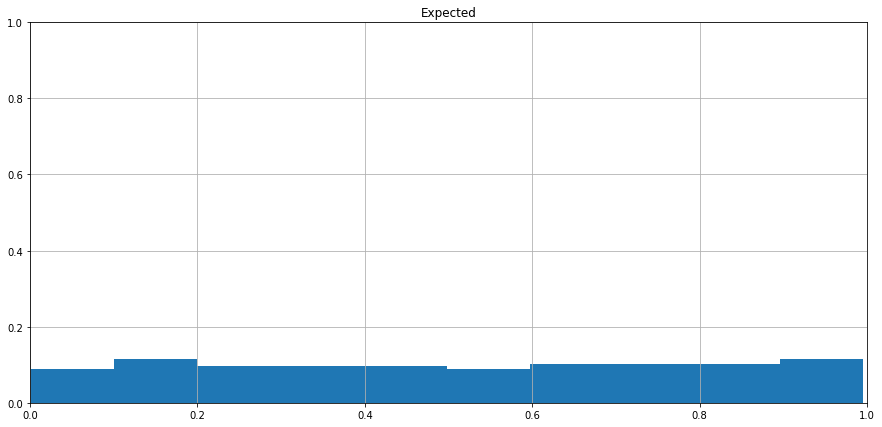
\includegraphics[width=\linewidth]{images/experiment_uniform_disgiunti/expected_memberships.png}
    \end{minipage}
    \begin{minipage}{0.48\textwidth}
        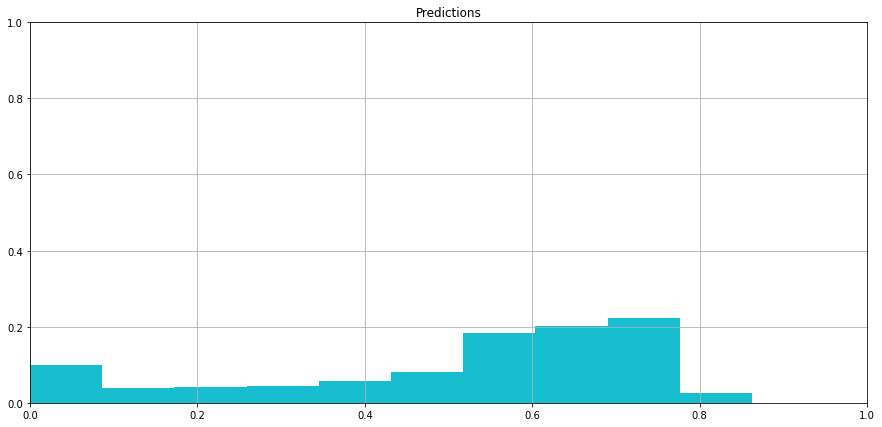
\includegraphics[width=\linewidth]{images/experiment_uniform_disgiunti/prediction_memberships.png}
    \end{minipage}
    \caption{A sinistra le etichette attese, a destra le predizioni effettuate da $\lambda$ nel primo esperimento.}
    \label{prediction_exp1}
\end{figure} 

Al fine di paragonare il comportamento dei modelli generati dall'algoritmo $\mu$-learn, sono state calcolate le predizioni da parte dell'algoritmo Random Forest (Figura~\ref{rf_exp1}). Tali predizioni sono state generate a partire dai migliori modelli selezionati tramite la grid search; i valori ottimali degli iperparametri dei modelli sono riportati in Tabella~\ref{models_rf_exp1}.

\begin{table}
\centering
\begin{adjustbox}{max width=\textwidth}
 \begin{tabular}{|c|c|c|c|c|c|} 
 \hline
\textbf{bootstrap} & \textbf{max profondità} & \textbf{max feature} & \textbf{min foglie campione} & \textbf{min partizioni campione} & \textbf{numero stimatori}
\\ [0.5ex] 
 \thickhline
 Sì & 80 & 3 & 4 & 8 & 1000 \\ 
 Sì & 80 & 3 & 4 & 8 & 100 \\ 
 Sì & 80 & 3 & 4 & 8 & 1000 \\ 
 Sì & 80 & 3 & 3 & 8 & 1000 \\ 
 Sì & 80 & 3 & 3 & 8 & 1000 \\ 
 \hline
\end{tabular}
\end{adjustbox}
\caption{Modelli migliori generati da Random Forest nel primo esperimento.}
\label{models_rf_exp1}
\end{table}

\begin{figure}
\centering
    \begin{minipage}{0.48\textwidth}
        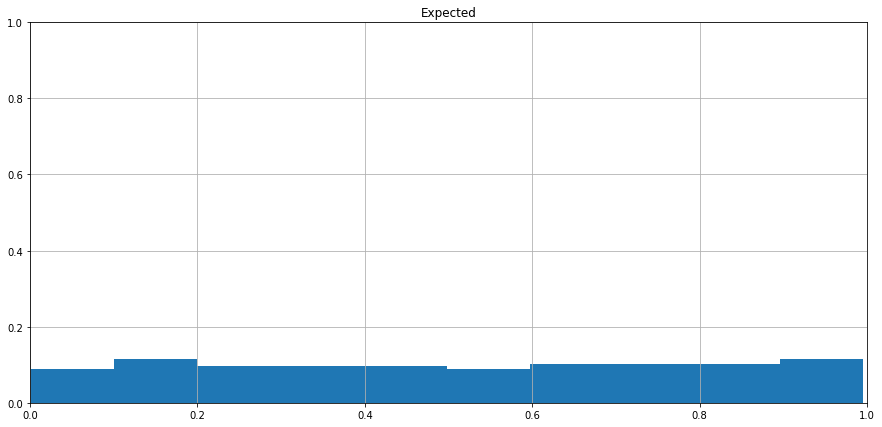
\includegraphics[width=\linewidth]{images/experiment_uniform_disgiunti/expected_memberships.png}
    \end{minipage}
    \begin{minipage}{0.48\textwidth}
        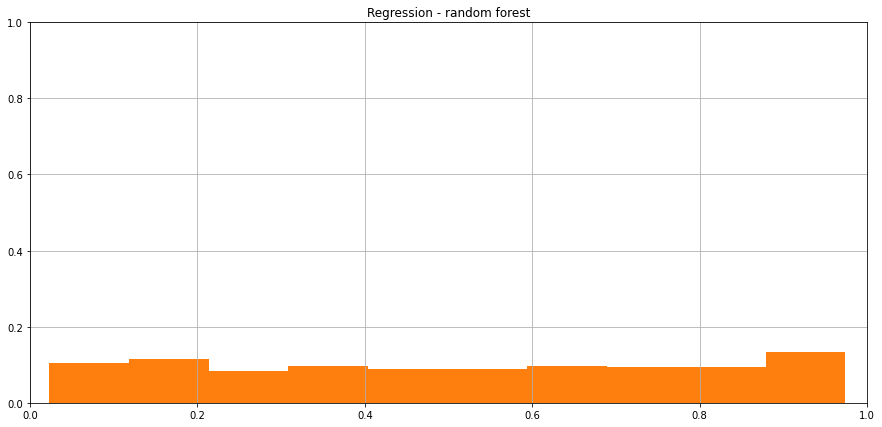
\includegraphics[width=\linewidth]{images/experiment_uniform_disgiunti/prediction_regression_rf.png}
    \end{minipage}
    \caption{A sinistra le etichette attese, a destra la regressione effettuata dall'algoritmo Random Forest nel primo esperimento.}
    \label{rf_exp1}
\end{figure} 
Dai grafici si evince chiaramente una notevole capacità da parte di Random Forest nel replicare fedelmente la distribuzione impostata per la generazione.
Per questa serie di esperimenti relativa ai dati generati sono stati calcolati i punteggi di RMSE per il training e il test error (Tabella~\ref{rmse_exp1}). 
\begin{table}
\centering
\begin{adjustbox}{max width=\textwidth}
 \begin{tabular}{|c|c|c|} 
 \hline
\textbf{Predittore} & \textbf{Training error} & \textbf{Test error}
\\ [0.5ex] 
 \thickhline
 $\lambda$ & 0.18 & 0.18 \\
 regressore random forest & \textbf{0.01} & \textbf{0.01}
 \\
 \hline
\end{tabular}
\end{adjustbox}
\caption{Valori di RMSE per il predittore $\lambda$ e Random Forest nel primo esperimento.}
\label{rmse_exp1}
\end{table}
I numeri confermano la superiorità da parte del regressore nell'individuare il grado di appartenenza originale dei documenti.

\paragraph{Confronto con $\bm{\omega}$}
Per quanto concerne la classificazione, in Figura~\ref{classification_exp1} viene fatto un primo confronto considerando il classificatore $\omega$. 
Più precisamente, in Figura~\ref{4cases_exp1} vengono mostrati i grafici relativi alle quattro classi presenti nella matrice di confusione.
Tali grafici mostrano l'andamento dei gradi di appartenenza ed esplicitano il comportamento di $\omega$ che effettua la classificazione in base alla classe preponderante.
\begin{figure}
\centering
    \begin{minipage}{0.48\textwidth}
        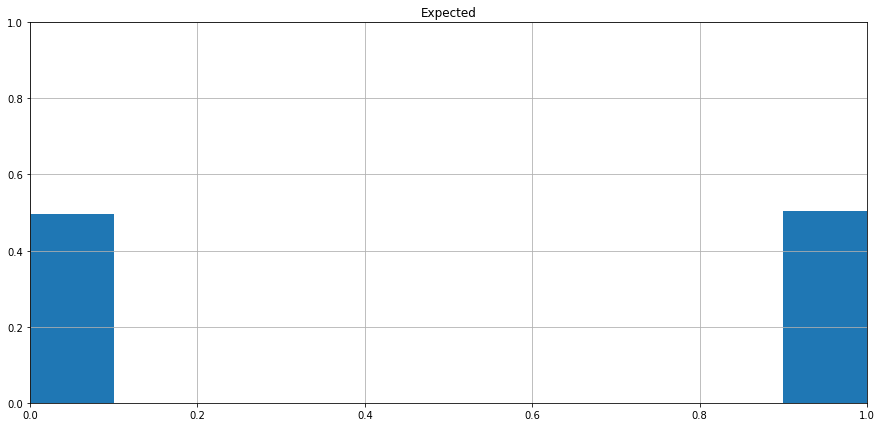
\includegraphics[width=\linewidth]{images/experiment_uniform_disgiunti/expected_classification.png}
    \end{minipage}
    \begin{minipage}{0.48\textwidth}
        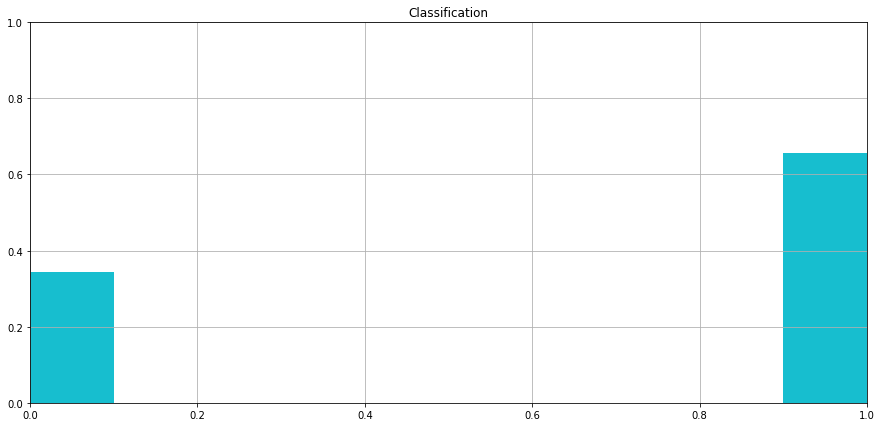
\includegraphics[width=\linewidth]{images/experiment_uniform_disgiunti/prediction_classification.png}
    \end{minipage}
    \caption{A sinistra le etichette attese, a destra le classificazioni effettuate da $\omega$ nel primo esperimento.}
    \label{classification_exp1}
\end{figure}
\begin{figure}
\centering
    \begin{minipage}{0.48\textwidth}
     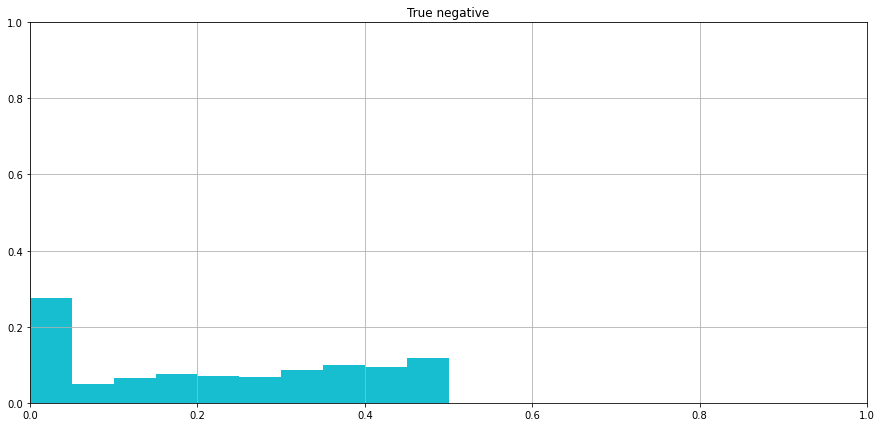
\includegraphics[width=\linewidth]{images/experiment_uniform_disgiunti/tn.png}\label{tn_ud}
   \end{minipage}
   \begin{minipage}{0.48\textwidth}
     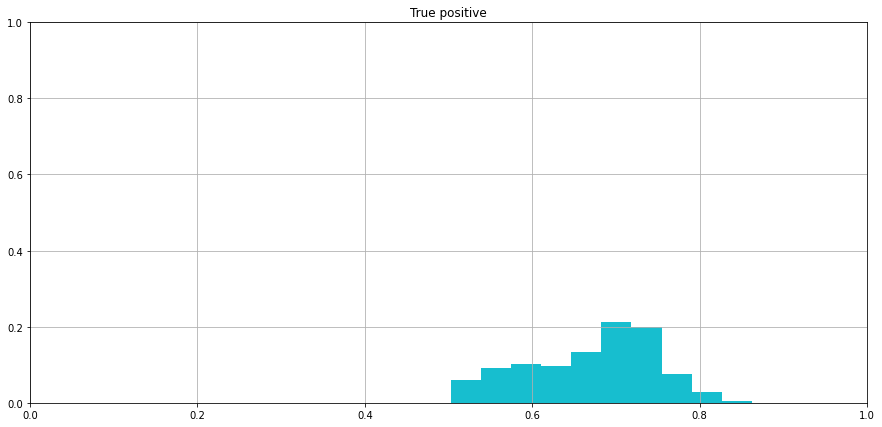
\includegraphics[width=\linewidth]{images/experiment_uniform_disgiunti/tp.png}\label{tp_ud}
   \end{minipage}
   \begin{minipage}{0.48\textwidth}
     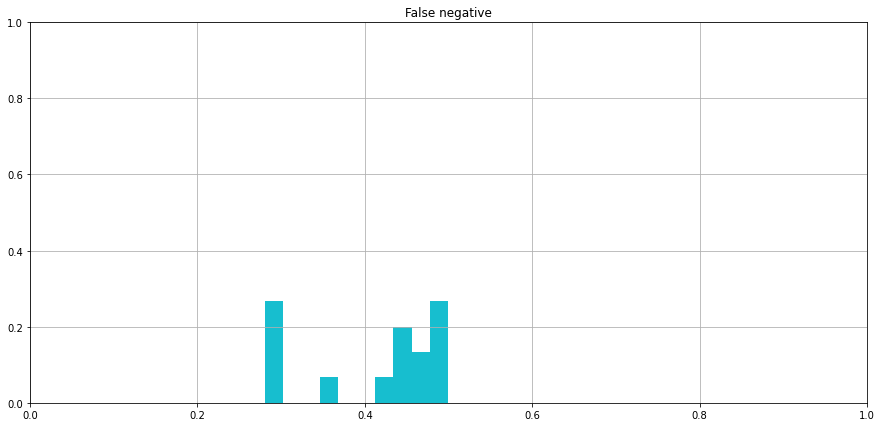
\includegraphics[width=\linewidth]{images/experiment_uniform_disgiunti/fn.png}\label{fn_ud}
   \end{minipage}
   \begin{minipage}{0.48\textwidth}
     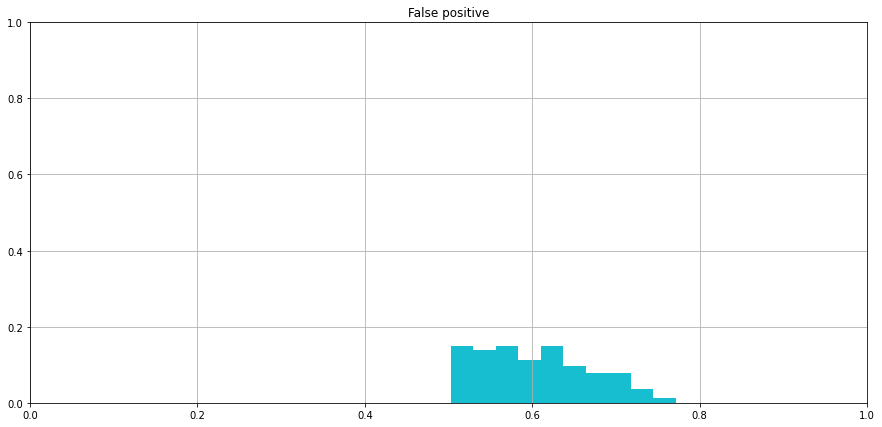
\includegraphics[width=\linewidth]{images/experiment_uniform_disgiunti/fp.png}\label{fp_ud}
   \end{minipage}
   \caption{In alto a sinistra i veri negativi, a destra i veri positivi; in basso a sinistra i falsi negativi e a destra i falsi positivi nel primo esperimento.}
   \label{4cases_exp1}
\end{figure}
 In Figura~\ref{rf_class_exp1}, invece, viene riportato il confronto tra le etichette attese e il classificatore Random Forest.

\begin{figure}
\centering
    \begin{minipage}{0.48\textwidth}
        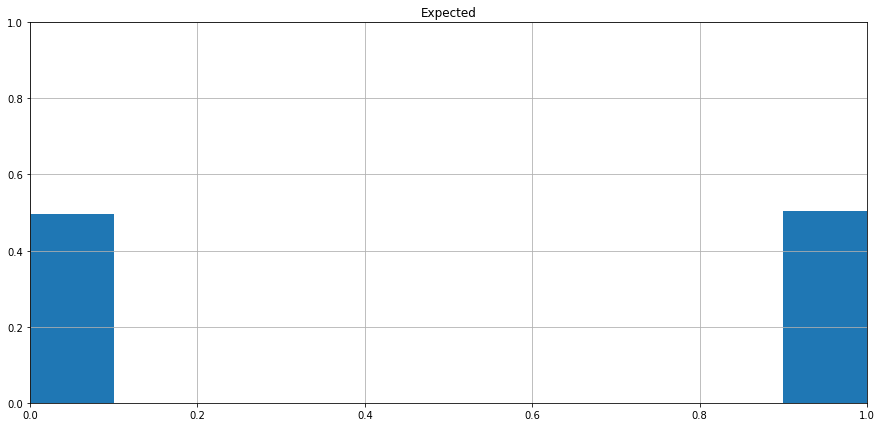
\includegraphics[width=\linewidth]{images/experiment_uniform_disgiunti/expected_classification.png}
    \end{minipage}
    \begin{minipage}{0.48\textwidth}
        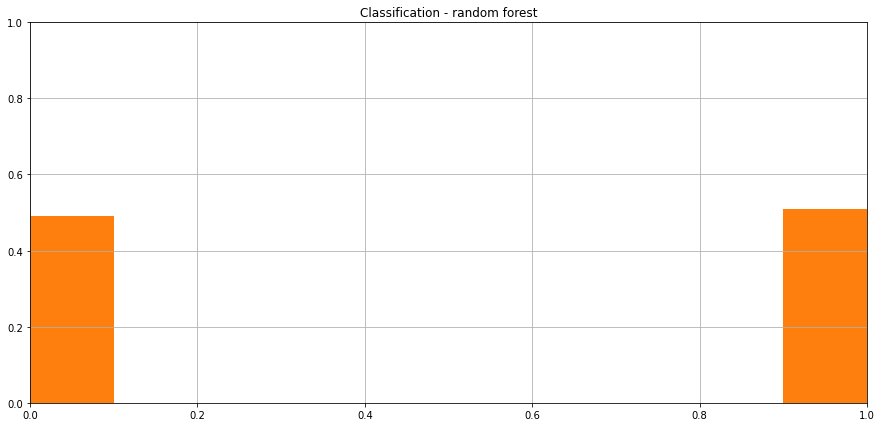
\includegraphics[width=\linewidth]{images/experiment_uniform_disgiunti/prediction_classification_rf.png}
    \end{minipage}
    \caption{A sinistra le etichette attese, a destra la classificazione effettuata da Random Forest nel primo esperimento.}
    \label{rf_class_exp1}
\end{figure} 
Anche in questo caso, l'algoritmo Random Forest si rivela particolarmente efficace. Si conferma questo aspetto nella Tabella~\ref{prf_exp1}, in cui vengono riportati i punteggi di Precision, Recall e F1.
\begin{table}
\centering
\begin{adjustbox}{max width=\textwidth}
 \begin{tabular}{|c|c|c|} 
 \hline
\textbf{Predittore} & \begin{tabular}{@{}c@{}}\textbf{Training} \\ \textbf{Precision}, \textbf{Recall}, \textbf{F1} \end{tabular} & \begin{tabular}{@{}c@{}}\textbf{Test} \\ \textbf{Precision}, \textbf{Recall}, \textbf{F1} \end{tabular}
\\ [0.5ex] 
 \thickhline
 $\omega$ & 0.75, 0.97, 0.85 & 0.77, 0.97, 0.86 \\
 classificatore random forest & \textbf{0.99, 1.0, 1.0} & \textbf{0.99, 0.99, 0.99} \\
 \hline
\end{tabular}
\end{adjustbox}
\caption{Valori di Precision, Recall e F1 per il predittore $\omega$ e la baseline nel primo esperimento.}
\label{prf_exp1}
\end{table}

\paragraph{Distribuzione beta con $\bm{\alpha=\beta=5}$}
Si prosegue utilizzando una distribuzione beta con parametri $\alpha=\beta=5$; i modelli selezionati vengono riportati nella Tabella~\ref{models_exp2}.
\begin{table}
\centering
\begin{adjustbox}{max width=\textwidth}
 \begin{tabular}{|c|c|c|c|c|} 
 \hline
\textbf{fuzzificatore} & \textbf{kernel} & \textbf{solver} & $\bm{\sigma}$ & \textit{\textbf{C}}
\\ [0.5ex] 
 \thickhline
 lineare & gaussiano & gurobi & 10 & 0.01 \\
 lineare & gaussiano & gurobi & 100000 & 10 \\
 lineare & gaussiano & gurobi & 1000 & 1 \\
 lineare & gaussiano & gurobi & 10 & 0.01 \\
 lineare & gaussiano & gurobi & 10 & 0.01 \\
 \hline
\end{tabular}
\end{adjustbox}
\caption{Modelli migliori generati da $\mu$-learn nel secondo esperimento.}
\label{models_exp2}
\end{table}
\paragraph{Confronto con $\bm{\lambda}$}
Analogamente a quanto fatto nel primo esperimento, si riporta in Figura~\ref{prediction_exp2} il confronto tra la ground truth dei dati generati e i gradi di appartenenza indotti dai modelli con il predittore $\lambda$.
\begin{figure}
\centering
    \begin{minipage}{0.48\textwidth}
        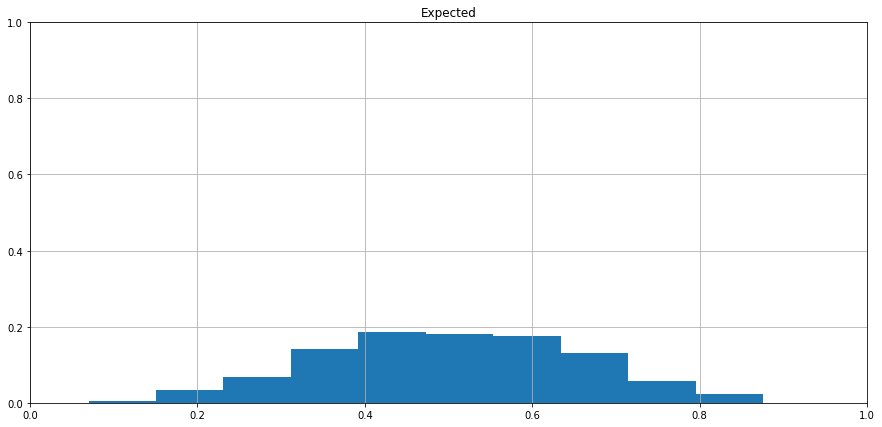
\includegraphics[width=\linewidth]{images/experiment_beta5_disgiunti/expected_memberships.png}
    \end{minipage}
    \begin{minipage}{0.48\textwidth}
        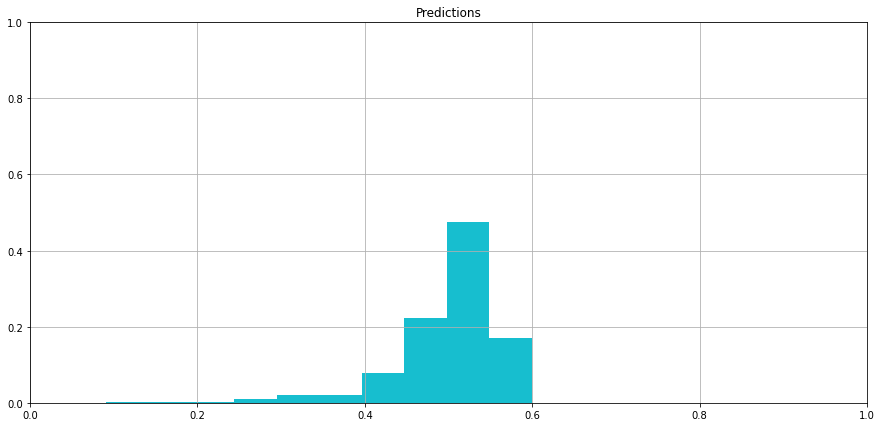
\includegraphics[width=\linewidth]{images/experiment_beta5_disgiunti/prediction_memberships.png}
    \end{minipage}
    \caption{A sinistra le etichette attese, a destra le predizioni effettuate da $\lambda$ nel secondo esperimento.}
    \label{prediction_exp2}
\end{figure} 

Anche in questo caso vengono raffigurate le predizioni dell'algoritmo Random Forest (Figura~\ref{rf_exp2}), per cui è stata eseguita la grid search per la ricerca dei parametri ottimali; i valori di tali parametri sono presenti in Tabella~\ref{models_rf_exp2}.

\begin{table}
\centering
\begin{adjustbox}{max width=\textwidth}
 \begin{tabular}{|c|c|c|c|c|c|} 
 \hline
\textbf{bootstrap} & \textbf{max profondità} & \textbf{max feature} & \textbf{min foglie campione} & \textbf{min partizioni campione} & \textbf{numero stimatori}
\\ [0.5ex] 
 \thickhline
 Sì & 80 & 3 & 3 & 10 & 200 \\ 
 Sì & 80 & 3 & 3 & 8 & 1000 \\ 
 Sì & 80 & 3 & 3 & 10 & 200 \\ 
 Sì & 80 & 3 & 3 & 12 & 300 \\ 
 Sì & 80 & 3 & 3 & 8 & 1000 \\ 
 \hline
\end{tabular}
\end{adjustbox}
\caption{Modelli migliori generati da Random Forest nel secondo esperimento.}
\label{models_rf_exp2}
\end{table}

\begin{figure}
\centering
    \begin{minipage}{0.48\textwidth}
        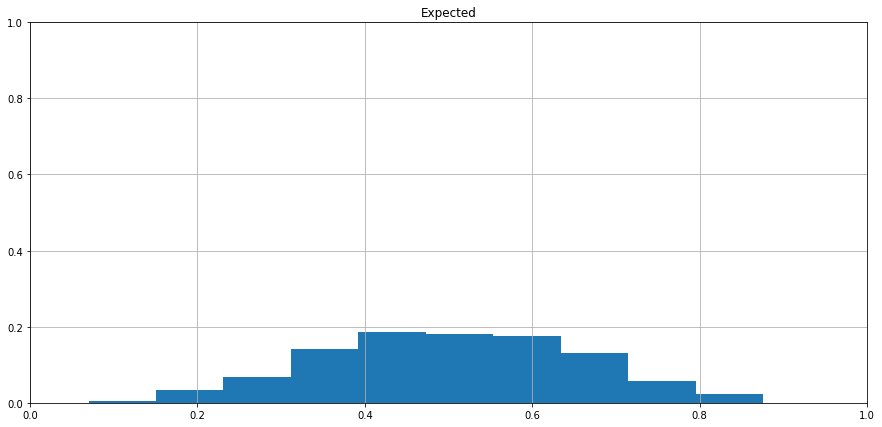
\includegraphics[width=\linewidth]{images/experiment_beta5_disgiunti/expected_memberships.png}
    \end{minipage}
    \begin{minipage}{0.48\textwidth}
        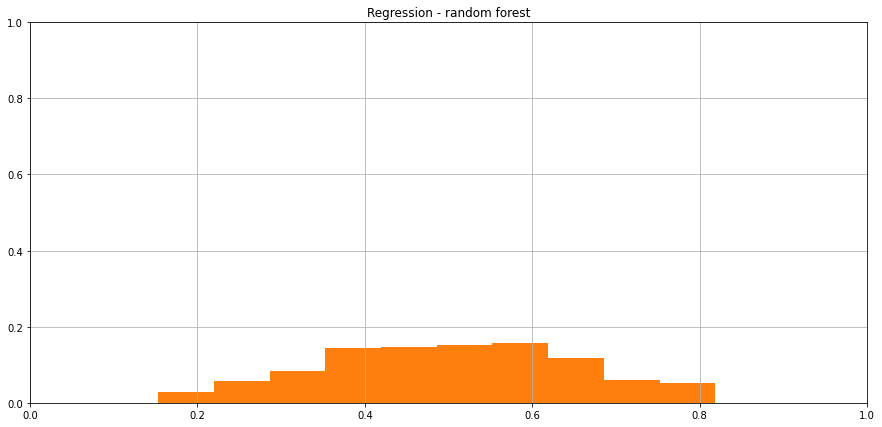
\includegraphics[width=\linewidth]{images/experiment_beta5_disgiunti/prediction_regression_rf.png}
    \end{minipage}
    \caption{A sinistra le etichette attese, a destra la regressione effettuata dall'algoritmo Random Forest nel secondo esperimento.}
    \label{rf_exp2}
\end{figure} 

Sono stati, dunque, calcolati i punteggi di RMSE per il training e il test error (Tabella~\ref{rmse_exp2}). 
\begin{table}
\centering
\begin{adjustbox}{max width=\textwidth}
 \begin{tabular}{|c|c|c|} 
 \hline
\textbf{Predittore} & \textbf{Training error} & \textbf{Test error}
\\ [0.5ex] 
 \thickhline
 $\lambda$ & 0.14 & 0.14 \\
 regressore random forest & \textbf{0.01} & \textbf{0.02}
 \\
 \hline
\end{tabular}
\end{adjustbox}
\caption{Valori di RMSE per il predittore $\lambda$ e Random Forest nel secondo esperimento nel secondo esperimento.}
\label{rmse_exp2}
\end{table}

\paragraph{Confronto con $\bm{\omega}$}
Nel caso della classificazione, si propone in Figura~\ref{classification_exp2} il confronto tra le etichette attese e le previsioni di $\omega$. 
In Figura~\ref{4cases_exp2} vengono mostrati i grafici inerenti alle quattro classi presenti nella matrice di confusione.
\begin{figure}
\centering
    \begin{minipage}{0.48\textwidth}
        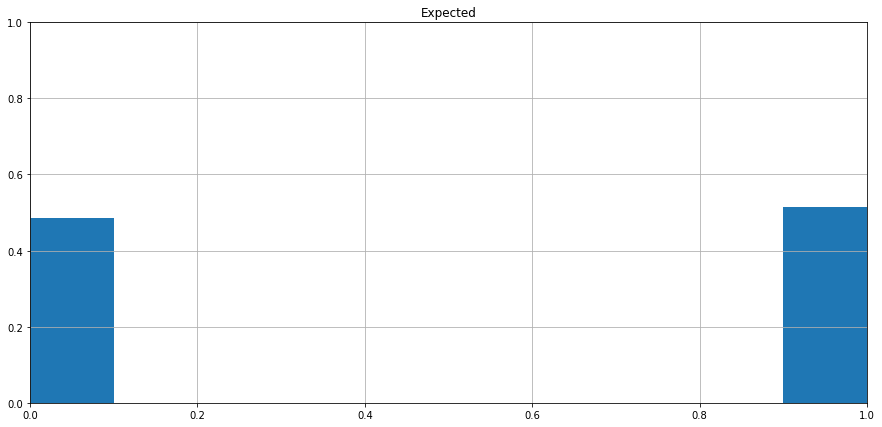
\includegraphics[width=\linewidth]{images/experiment_beta5_disgiunti/expected_classification.png}
    \end{minipage}
    \begin{minipage}{0.48\textwidth}
        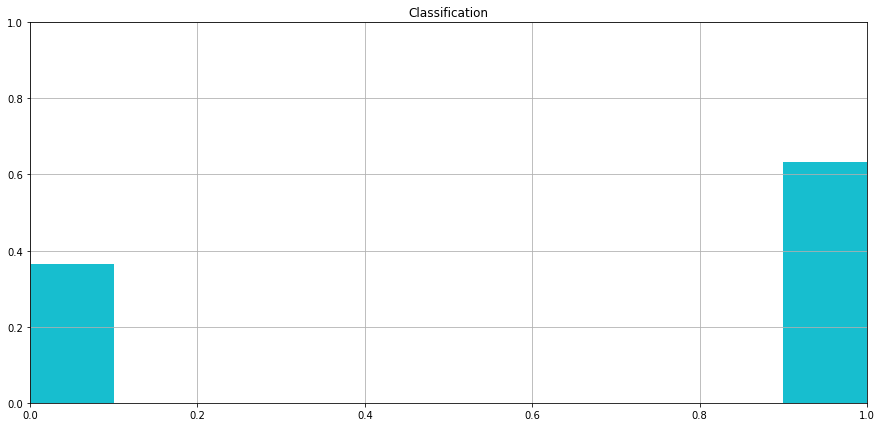
\includegraphics[width=\linewidth]{images/experiment_beta5_disgiunti/prediction_classification.png}
    \end{minipage}
    \caption{A sinistra le etichette attese, a destra le classificazioni effettuate da $\omega$ nel secondo esperimento.}
    \label{classification_exp2}
\end{figure}
\begin{figure}
\centering
    \begin{minipage}{0.48\textwidth}
     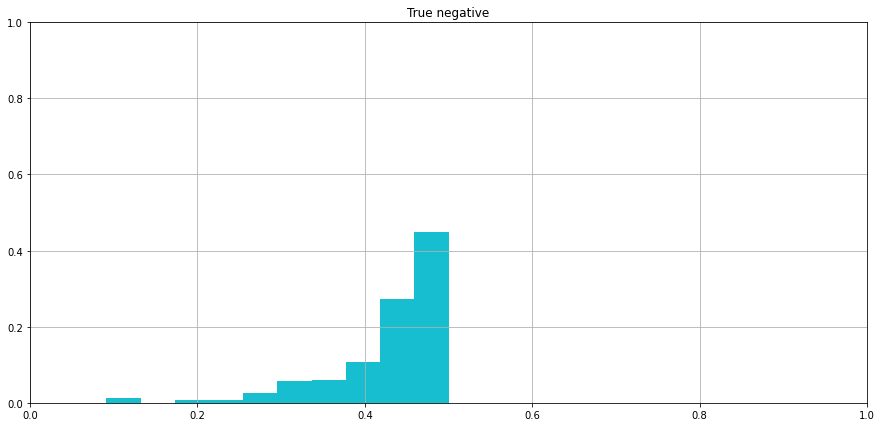
\includegraphics[width=\linewidth]{images/experiment_beta5_disgiunti/tn.png}\label{tn_b5d}
   \end{minipage}
   \begin{minipage}{0.48\textwidth}
     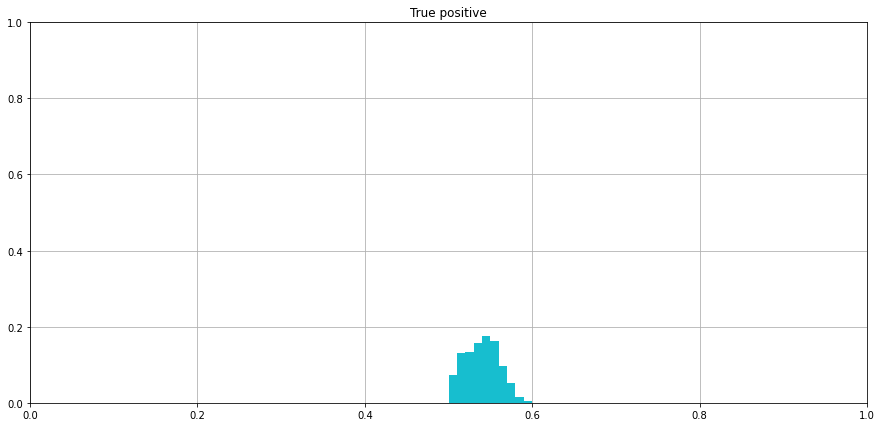
\includegraphics[width=\linewidth]{images/experiment_beta5_disgiunti/tp.png}\label{tp_b5d}
   \end{minipage}
   \begin{minipage}{0.48\textwidth}
     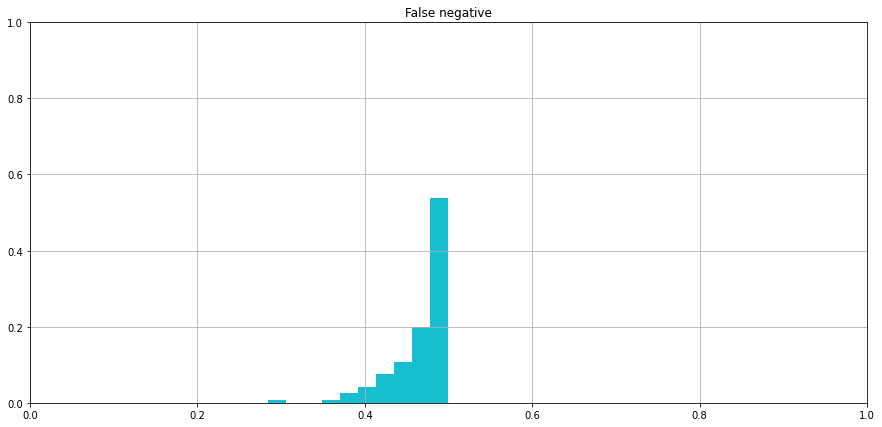
\includegraphics[width=\linewidth]{images/experiment_beta5_disgiunti/fn.png}\label{fn_b5d}
   \end{minipage}
   \begin{minipage}{0.48\textwidth}
     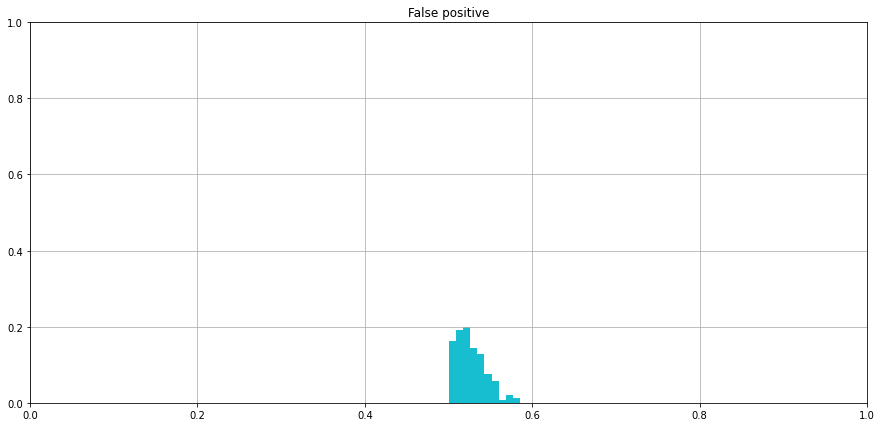
\includegraphics[width=\linewidth]{images/experiment_beta5_disgiunti/fp.png}\label{fp_b5d}
   \end{minipage}
   \caption{In alto a sinistra i veri negativi, a destra i veri positivi; in basso a sinistra i falsi negativi e a destra i falsi positivi nel secondo esperimento.}
   \label{4cases_exp2}
\end{figure}
In Figura~\ref{rf_class_exp2} viene riportato il confronto tra le etichette attese e il classificatore Random Forest in arancione.

\begin{figure}
\centering
    \begin{minipage}{0.48\textwidth}
        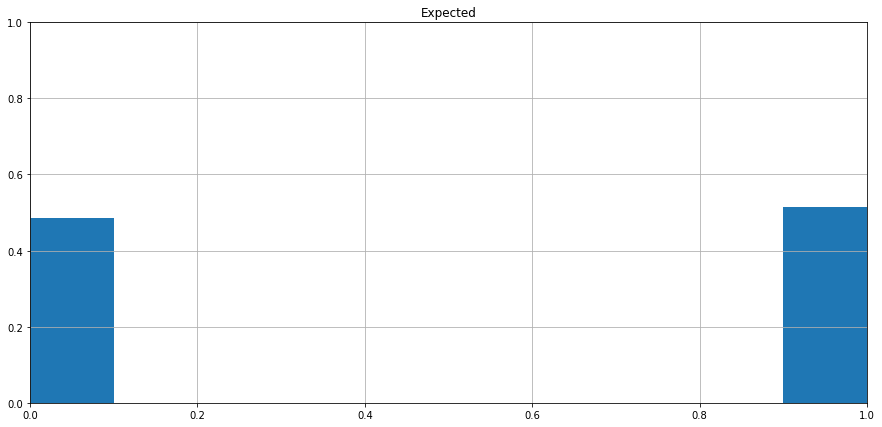
\includegraphics[width=\linewidth]{images/experiment_beta5_disgiunti/expected_classification.png}
    \end{minipage}
    \begin{minipage}{0.48\textwidth}
        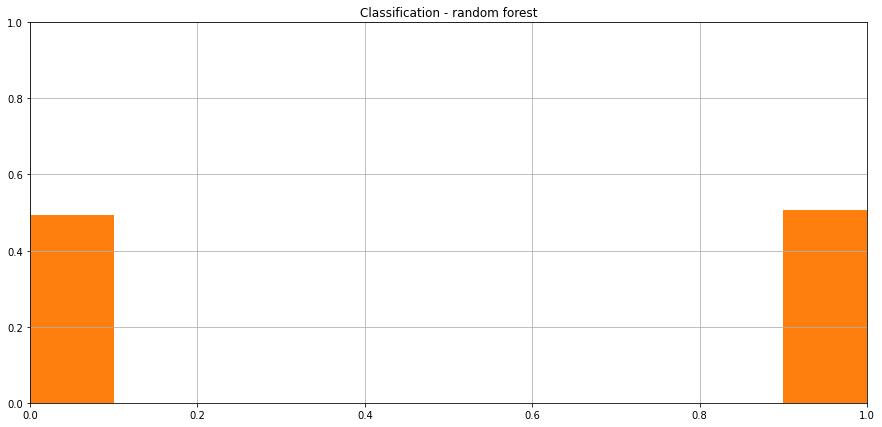
\includegraphics[width=\linewidth]{images/experiment_beta5_disgiunti/prediction_classification_rf.png}
    \end{minipage}
    \caption{A sinistra le etichette attese, a destra la classificazione effettuata da Random Forest nel secondo esperimento.}
    \label{rf_class_exp2}
\end{figure} 
In Tabella~\ref{prf_exp2} vengono riportati i punteggi di Precision, Recall e F1.
\begin{table}
\centering
\begin{adjustbox}{max width=\textwidth}
 \begin{tabular}{|c|c|c|} 
 \hline
\textbf{Predittore} & \begin{tabular}{@{}c@{}}\textbf{Training} \\ \textbf{Precision}, \textbf{Recall}, \textbf{F1} \end{tabular} & \begin{tabular}{@{}c@{}}\textbf{Test} \\ \textbf{Precision}, \textbf{Recall}, \textbf{F1} \end{tabular}
\\ [0.5ex] 
 \thickhline
 $\omega$ & 0.62, 0.77, 0.69 & 0.63, 0.77, 0.69 \\
 classificatore random forest & \textbf{0.99, 0.98, 0.98} & \textbf{0.98, 0.96, 0.97} \\
 \hline
\end{tabular}
\end{adjustbox}
\caption{Valori di Precision, Recall e F1 per il predittore $\omega$ e la baseline nel secondo esperimento.}
\label{prf_exp2}
\end{table}
Da un punto di vista dell'efficacia dei due modelli, si confermano le considerazioni fatte per il primo esperimento.

\paragraph{Distribuzione beta con $\bm{\alpha=\beta=0.5}$}
Il terzo caso parte da una distribuzione beta con parametri $\alpha=\beta=0.5$ e i modelli scelti vengono mostrati nella Tabella~\ref{models_exp3}.
\begin{table}
\centering
\begin{adjustbox}{max width=\textwidth}
 \begin{tabular}{|c|c|c|c|c|} 
 \hline
\textbf{fuzzificatore} & \textbf{kernel} & \textbf{solver} & $\bm{\sigma}$ & \textit{\textbf{C}}
\\ [0.5ex] 
 \thickhline
 lineare & gaussiano & gurobi & 10 & 0.01 \\
 lineare & gaussiano & gurobi & 10 & 0.01 \\
 lineare & gaussiano & gurobi & 10 & 0.01 \\
 lineare & gaussiano & gurobi & 10 & 0.01 \\
 lineare & gaussiano & gurobi & 10 & 0.01 \\
 \hline
\end{tabular}
\end{adjustbox}
\caption{Modelli migliori generati da $\mu$-learn nel terzo esperimento.}
\label{models_exp3}
\end{table}
\paragraph{Confronto con $\bm{\lambda}$}
Al fine di visualizzare il comportamento di $\lambda$, viene mostrato in Figura~\ref{prediction_exp3} il confronto tra le predizioni generate da tale predittore e la ground truth.
\begin{figure}
\centering
    \begin{minipage}{0.48\textwidth}
        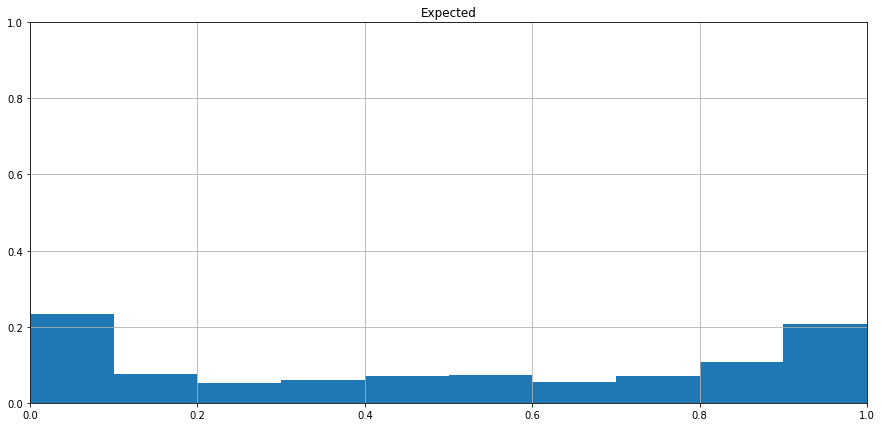
\includegraphics[width=\linewidth]{images/experiment_beta05_disgiunti/expected_memberships.png}
    \end{minipage}
    \begin{minipage}{0.48\textwidth}
        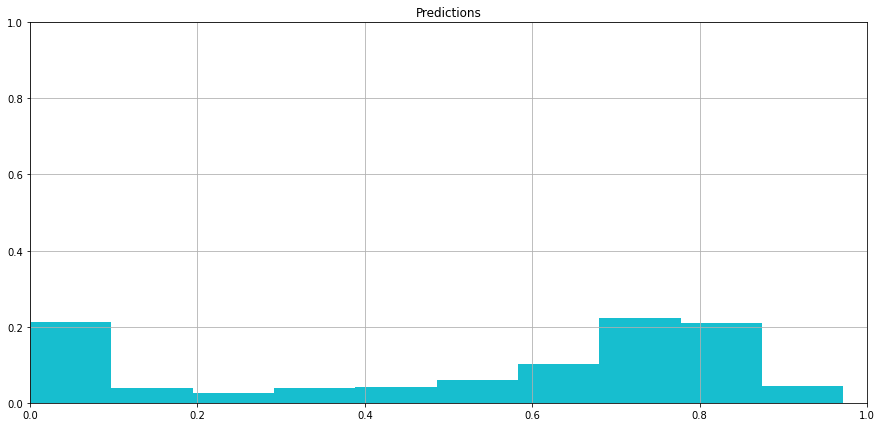
\includegraphics[width=\linewidth]{images/experiment_beta05_disgiunti/prediction_memberships.png}
    \end{minipage}
    \caption{A sinistra le etichette attese, a destra le predizioni effettuate da $\lambda$ nel terzo esperimento.}
    \label{prediction_exp3}
\end{figure} 

In Figura~\ref{rf_exp3} è possibile osservare il comportamento dei modelli ottenuti tramite Random Forest; essi vengono elencati in Tabella~\ref{models_rf_exp3}.

\begin{table}
\centering
\begin{adjustbox}{max width=\textwidth}
 \begin{tabular}{|c|c|c|c|c|c|} 
 \hline
\textbf{bootstrap} & \textbf{max profondità} & \textbf{max feature} & \textbf{min foglie campione} & \textbf{min partizioni campione} & \textbf{numero stimatori}
\\ [0.5ex] 
 \thickhline
 Sì & 80 & 3 & 3 & 8 & 1000 \\ 
 Sì & 80 & 3 & 3 & 8 & 1000 \\ 
 Sì & 80 & 3 & 3 & 8 & 1000 \\ 
 Sì & 80 & 3 & 3 & 10 & 300 \\ 
 Sì & 80 & 3 & 3 & 8 & 1000 \\ 
 \hline
\end{tabular}
\end{adjustbox}
\caption{Modelli migliori generati da Random Forest nel terzo esperimento.}
\label{models_rf_exp3}
\end{table}

\begin{figure}
\centering
    \begin{minipage}{0.48\textwidth}
        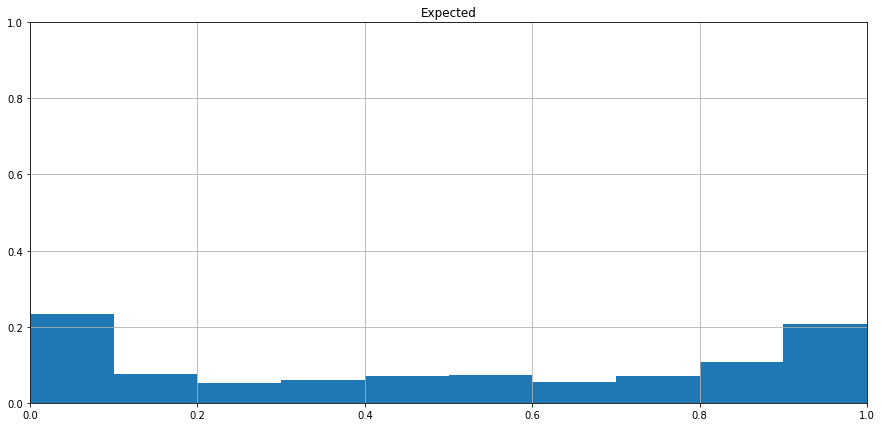
\includegraphics[width=\linewidth]{images/experiment_beta05_disgiunti/expected_memberships.png}
    \end{minipage}
    \begin{minipage}{0.48\textwidth}
        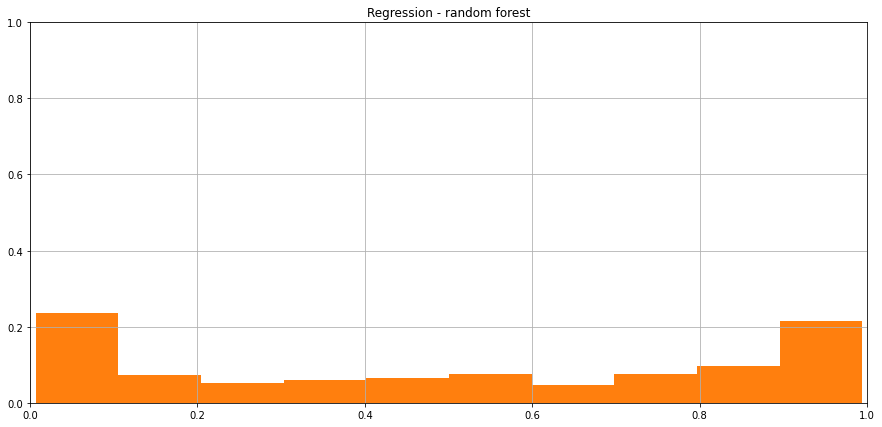
\includegraphics[width=\linewidth]{images/experiment_beta05_disgiunti/prediction_regression_rf.png}
    \end{minipage}
    \caption{A sinistra le etichette attese, a destra la regressione effettuata dall'algoritmo Random Forest nel terzo esperimento.}
    \label{rf_exp3}
\end{figure} 
I punteggi di RMSE per il training e il test error sono riportati in Tabella~\ref{rmse_exp3}.

\begin{table}
\centering
\begin{adjustbox}{max width=\textwidth}
 \begin{tabular}{|c|c|c|} 
 \hline
\textbf{Predittore} & \textbf{Training error} & \textbf{Test error}
\\ [0.5ex] 
 \thickhline
 $\lambda$ & 0.14 & 0.14 \\
 regressore random forest & \textbf{0.01} & \textbf{0.02}
 \\
 \hline
\end{tabular}
\end{adjustbox}
\caption{Valori di RMSE per il predittore $\lambda$ e Random Forest nel secondo esperimento nel terzo esperimento.}
\label{rmse_exp3}
\end{table}

\paragraph{Confronto con $\bm{\omega}$}
Nel caso del classificatore $\omega$ si osserva in Figura~\ref{classification_exp3} il confronto con le etichette attese. 
In Figura~\ref{4cases_exp3} vengono mostrati i grafici relativi ai veri negativi, veri positivi, falsi negativi e falsi positivi.
\begin{figure}
\centering
    \begin{minipage}{0.48\textwidth}
        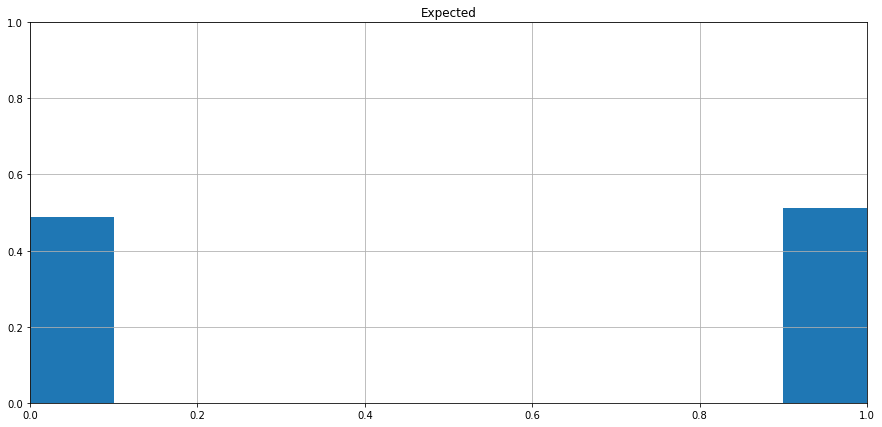
\includegraphics[width=\linewidth]{images/experiment_beta05_disgiunti/expected_classification.png}
    \end{minipage}
    \begin{minipage}{0.48\textwidth}
        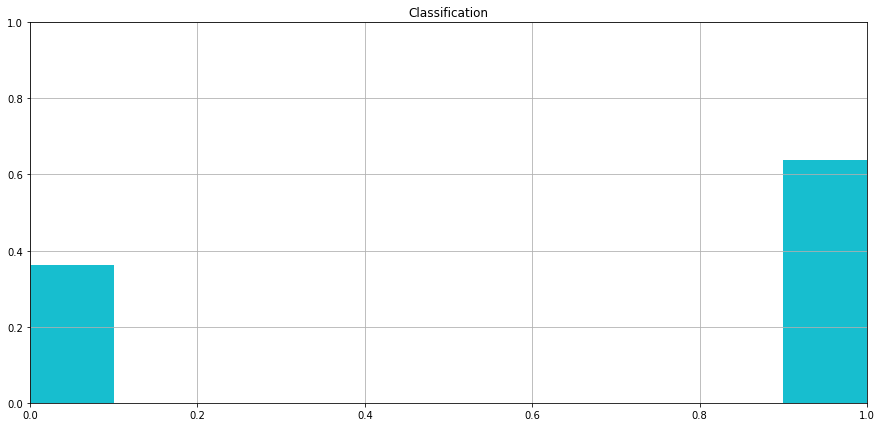
\includegraphics[width=\linewidth]{images/experiment_beta05_disgiunti/prediction_classification.png}
    \end{minipage}
    \caption{A sinistra le etichette attese, a destra le classificazioni effettuate da $\omega$ nel terzo esperimento.}
    \label{classification_exp3}
\end{figure}
\begin{figure}
\centering
    \begin{minipage}{0.48\textwidth}
     \includegraphics[width=\linewidth]{images/experiment_beta05_disgiunti/tn.png}\label{tn_b05d}
   \end{minipage}
   \begin{minipage}{0.48\textwidth}
     \includegraphics[width=\linewidth]{images/experiment_beta05_disgiunti/tp.png}\label{tp_b05d}
   \end{minipage}
   \begin{minipage}{0.48\textwidth}
     \includegraphics[width=\linewidth]{images/experiment_beta05_disgiunti/fn.png}\label{fn_b05d}
   \end{minipage}
   \begin{minipage}{0.48\textwidth}
     \includegraphics[width=\linewidth]{images/experiment_beta05_disgiunti/fp.png}\label{fp_b05d}
   \end{minipage}
   \caption{In alto a sinistra i veri negativi, a destra i veri positivi; in basso a sinistra i falsi negativi e a destra i falsi positivi nel terzo esperimento.}
   \label{4cases_exp3}
\end{figure}
In Figura~\ref{rf_class_exp3} vengono visualizzate le predizioni di Random Forest su questo tipo di distribuzione.

\begin{figure}
\centering
    \begin{minipage}{0.48\textwidth}
        \includegraphics[width=\linewidth]{images/experiment_beta05_disgiunti/expected_classification.png}
    \end{minipage}
    \begin{minipage}{0.48\textwidth}
        \includegraphics[width=\linewidth]{images/experiment_beta05_disgiunti/prediction_classification_rf.png}
    \end{minipage}
    \caption{A sinistra le etichette attese, a destra la classificazione effettuata da Random Forest nel terzo esperimento.}
    \label{rf_class_exp3}
\end{figure} 
Si chiude questa prima parte di esperimenti con la Tabella~\ref{prf_exp3} relativa ai punteggi di Precision, Recall e F1.
\begin{table}
\centering
\begin{adjustbox}{max width=\textwidth}
 \begin{tabular}{|c|c|c|} 
 \hline
\textbf{Predittore} & \begin{tabular}{@{}c@{}}\textbf{Training} \\ \textbf{Precision}, \textbf{Recall}, \textbf{F1} \end{tabular} & \begin{tabular}{@{}c@{}}\textbf{Test} \\ \textbf{Precision}, \textbf{Recall}, \textbf{F1} \end{tabular}
\\ [0.5ex] 
 \thickhline
 $\omega$ & 0.62, 0.77, 0.69 & 0.63, 0.77, 0.69 \\
 classificatore random forest & \textbf{1.0, 0.99, 1.0} & \textbf{0.99, 0.99, 0.99} \\
 \hline
\end{tabular}
\end{adjustbox}
\caption{Valori di Precision, Recall e F1 per il predittore $\omega$ e la baseline nel terzo esperimento.}
\label{prf_exp3}
\end{table}
L'algoritmo Random Forest si rivela particolarmente efficace anche in questo caso, riuscendo a riprodurre fedelmente la distribuzione di partenza e compiendo un errore davvero contenuto.
I modelli generati da $\mu$-learn rivelano dei punteggi accettabili sia nel caso della classificazione che dell'induzione del grado di appartenenza, tuttavia nel confronto con la baseline risultano fin qui inferiori.


\subsubsection{Insiemi sovrapposti}\label{insiemisovrapposti}
L'altra sequenza di esperimenti si basa su insiemi di parole di partenza con una componente di sovrapposizione del $17\%$. Anche in questo caso gli esperimenti si articolano nelle tre distribuzioni utilizzate in precedenza. Lo scopo di questa parte di esperimenti è vedere come variano i risultati.

\paragraph{Distribuzione uniforme} Analogamente alla distribuzione uniforme continua nell'intervallo $[0,1]$ vista per gli insiemi disgiunti (Paragrafo~\ref{insiemidisgiunti}), si utilizza tale distribuzione per gli insiemi sovrapposti. In Tabella~\ref{models_exp4} vengono menzionati quali modelli siano stati reputati ottimali per questo tipo di dati.
\begin{table}
\centering
\begin{adjustbox}{max width=\textwidth}
 \begin{tabular}{|c|c|c|c|c|} 
 \hline
\textbf{fuzzificatore} & \textbf{kernel} & \textbf{solver} & $\bm{\sigma}$ & \textit{\textbf{C}}
\\ [0.5ex] 
 \thickhline
 lineare & gaussiano & gurobi & 1000 & 100 \\
 lineare & gaussiano & gurobi & 1000 & 100 \\
 lineare & gaussiano & gurobi & 1000 & 10 \\
 lineare & gaussiano & gurobi & 1000 & 100 \\
 lineare & gaussiano & gurobi & 1000 & 100 \\
 \hline
\end{tabular}
\end{adjustbox}
\caption{Modelli migliori generati da $\mu$-learn nel quarto esperimento.}
\label{models_exp4}
\end{table}
\paragraph{Confronto con $\bm{\lambda}$}
In Figura~\ref{prediction_exp4} è raffigurato il comportamento di $\lambda$ nel generare le predizioni e il risultato è pressoché identico a quello ritrovato nel caso di insiemi disgiunti.
\begin{figure}
\centering
    \begin{minipage}{0.48\textwidth}
        \includegraphics[width=\linewidth]{images/experiment_uniform_sovrapposti/expected_memberships.png}
    \end{minipage}
    \begin{minipage}{0.48\textwidth}
        \includegraphics[width=\linewidth]{images/experiment_uniform_sovrapposti/prediction_memberships.png}
    \end{minipage}
    \caption{A sinistra le etichette attese, a destra le predizioni effettuate da $\lambda$ nel quarto esperimento.}
    \label{prediction_exp4}
\end{figure} 
Le predizioni dell'algoritmo Random Forest vengono mostrate in Figura~\ref{rf_exp4} e sono relative ai modelli riportati in Tabella~\ref{models_rf_exp4}.

\begin{table}
\centering
\begin{adjustbox}{max width=\textwidth}
 \begin{tabular}{|c|c|c|c|c|c|} 
 \hline
\textbf{bootstrap} & \textbf{max profondità} & \textbf{max feature} & \textbf{min foglie campione} & \textbf{min partizioni campione} & \textbf{numero stimatori}
\\ [0.5ex] 
 \thickhline
 Sì & 80 & 3 & 3 & 8 & 100 \\ 
 Sì & 80 & 3 & 3 & 8 & 100 \\ 
 Sì & 80 & 3 & 4 & 10 & 100 \\ 
 Sì & 80 & 3 & 3 & 8 & 100 \\ 
 Sì & 80 & 3 & 3 & 8 & 100 \\ 
 \hline
\end{tabular}
\end{adjustbox}
\caption{Modelli migliori generati da Random Forest nel quarto esperimento.}
\label{models_rf_exp4}
\end{table}

\begin{figure}
\centering
    \begin{minipage}{0.48\textwidth}
        \includegraphics[width=\linewidth]{images/experiment_uniform_sovrapposti/expected_memberships.png}
    \end{minipage}
    \begin{minipage}{0.48\textwidth}
        \includegraphics[width=\linewidth]{images/experiment_uniform_sovrapposti/prediction_regression_rf.png}
    \end{minipage}
    \caption{A sinistra le etichette attese, a destra la regressione effettuata dall'algoritmo Random Forest nel quarto esperimento.}
    \label{rf_exp4}
\end{figure} 

Successivamente, si mostrano in Tabella~\ref{rmse_exp4} i punteggi di RMSE per il training e il test error. 
\begin{table}
\centering
\begin{adjustbox}{max width=\textwidth}
 \begin{tabular}{|c|c|c|} 
 \hline
\textbf{Predittore} & \textbf{Training error} & \textbf{Test error}
\\ [0.5ex] 
 \thickhline
 $\lambda$ & 0.20 & 0.21 \\
 regressore random forest & \textbf{0.02} & \textbf{0.03}
 \\
 \hline
\end{tabular}
\end{adjustbox}
\caption{Valori di RMSE per il predittore $\lambda$ e Random Forest nel quarto esperimento.}
\label{rmse_exp4}
\end{table}

\paragraph{Confronto con $\bm{\omega}$}
In Figura~\ref{classification_exp4} si passa nuovamente al caso del classificatore $\omega$ per insiemi sovrapposti, approfondendo nel dettaglio in Figura~\ref{4cases_exp4} i grafici relativi alle quattro classi presenti nella matrice di confusione.
\begin{figure}
\centering
    \begin{minipage}{0.48\textwidth}
        \includegraphics[width=\linewidth]{images/experiment_uniform_sovrapposti/expected_classification.png}
    \end{minipage}
    \begin{minipage}{0.48\textwidth}
        \includegraphics[width=\linewidth]{images/experiment_uniform_sovrapposti/prediction_classification.png}
    \end{minipage}
    \caption{A sinistra le etichette attese, a destra le classificazioni effettuate da $\omega$ nel quarto esperimento.}
    \label{classification_exp4}
\end{figure}
\begin{figure}
\centering
    \begin{minipage}{0.48\textwidth}
     \includegraphics[width=\linewidth]{images/experiment_uniform_sovrapposti/tn.png}\label{tn_us}
   \end{minipage}
   \begin{minipage}{0.48\textwidth}
     \includegraphics[width=\linewidth]{images/experiment_uniform_sovrapposti/tp.png}\label{tp_us}
   \end{minipage}
   \begin{minipage}{0.48\textwidth}
     \includegraphics[width=\linewidth]{images/experiment_uniform_sovrapposti/fn.png}\label{fn_us}
   \end{minipage}
   \begin{minipage}{0.48\textwidth}
     \includegraphics[width=\linewidth]{images/experiment_uniform_sovrapposti/fp.png}\label{fp_us}
   \end{minipage}
   \caption{In alto a sinistra i veri negativi, a destra i veri positivi; in basso a sinistra i falsi negativi e a destra i falsi positivi nel quarto esperimento.}
   \label{4cases_exp4}
\end{figure}
Per quanto riguarda le previsioni dell'algoritmo Random Forest, in Figura~\ref{rf_class_exp4} viene riportato il confronto con la ground truth.

\begin{figure}
\centering
    \begin{minipage}{0.48\textwidth}
        \includegraphics[width=\linewidth]{images/experiment_uniform_sovrapposti/expected_classification.png}
    \end{minipage}
    \begin{minipage}{0.48\textwidth}
        \includegraphics[width=\linewidth]{images/experiment_uniform_sovrapposti/prediction_classification_rf.png}
    \end{minipage}
    \caption{A sinistra le etichette attese, a destra la classificazione effettuata da Random Forest nel quarto esperimento.}
    \label{rf_class_exp4}
\end{figure} 
Di conseguenza, si mostrano i relativi punteggi di Precision, Recall e F1 in Tabella~\ref{prf_exp4}.
\begin{table}
\centering
\begin{adjustbox}{max width=\textwidth}
 \begin{tabular}{|c|c|c|} 
 \hline
\textbf{Predittore} & \begin{tabular}{@{}c@{}}\textbf{Training} \\ \textbf{Precision}, \textbf{Recall}, \textbf{F1} \end{tabular} & \begin{tabular}{@{}c@{}}\textbf{Test} \\ \textbf{Precision}, \textbf{Recall}, \textbf{F1} \end{tabular}
\\ [0.5ex] 
 \thickhline
 $\omega$ & 0.73, 0.91, 0.81 & 0.75, 0.86, 0.80 \\
 classificatore random forest & \textbf{0.99, 0.99, 0.99} & \textbf{0.98, 0.98, 0.98} \\
 \hline
\end{tabular}
\end{adjustbox}
\caption{Valori di Precision, Recall e F1 per il predittore $\omega$ e la baseline nel quarto esperimento.}
\label{prf_exp4}
\end{table}

\paragraph{Distribuzione beta con $\bm{\alpha=\beta=5}$}
Nel caso della distribuzione beta con parametri $\alpha=\beta=5$ per insiemi sovrapposti, i modelli scelti tramite la grid search vengono riportati nella Tabella~\ref{models_exp5}.
\begin{table}
\centering
\begin{adjustbox}{max width=\textwidth}
 \begin{tabular}{|c|c|c|c|c|} 
 \hline
\textbf{fuzzificatore} & \textbf{kernel} & \textbf{solver} & $\bm{\sigma}$ & \textit{\textbf{C}}
\\ [0.5ex] 
 \thickhline
 lineare & gaussiano & gurobi & 1000 & 1 \\
 lineare & gaussiano & gurobi & 1000 & 1 \\
 lineare & gaussiano & gurobi & 1000 & 1 \\
 lineare & gaussiano & gurobi & 1000 & 1 \\
 lineare & gaussiano & gurobi & 1000 & 1 \\
 \hline
\end{tabular}
\end{adjustbox}
\caption{Modelli migliori generati da $\mu$-learn nel quinto esperimento.}
\label{models_exp5}
\end{table}
\paragraph{Confronto con $\bm{\lambda}$}
In Figura~\ref{prediction_exp5} si visualizza i grafici della ground truth dei dati generati e dei gradi di appartenenza trovati dai modelli con il predittore $\lambda$.
\begin{figure}
\centering
    \begin{minipage}{0.48\textwidth}
        \includegraphics[width=\linewidth]{images/experiment_beta5_sovrapposti/expected_memberships.png}
    \end{minipage}
    \begin{minipage}{0.48\textwidth}
        \includegraphics[width=\linewidth]{images/experiment_beta5_sovrapposti/prediction_memberships.png}
    \end{minipage}
    \caption{A sinistra le etichette attese, a destra le predizioni effettuate da $\lambda$ nel quinto esperimento.}
    \label{prediction_exp5}
\end{figure} 
La grid search è stata applicata anche all'algoritmo Random Forest, generando i modelli riassunti in Tabella~\ref{models_rf_exp5}; tali modelli hanno prodotto le previsioni mostrate in Figura~\ref{rf_exp5}.
\begin{table}
\centering
\begin{adjustbox}{max width=\textwidth}
 \begin{tabular}{|c|c|c|c|c|c|} 
 \hline
\textbf{bootstrap} & \textbf{max profondità} & \textbf{max feature} & \textbf{min foglie campione} & \textbf{min partizioni campione} & \textbf{numero stimatori}
\\ [0.5ex] 
 \thickhline
 Sì & 80 & 3 & 3 & 8 & 300 \\ 
 Sì & 80 & 3 & 4 & 8 & 1000 \\ 
 Sì & 80 & 3 & 3 & 8 & 300 \\ 
 Sì & 80 & 3 & 3 & 8 & 100 \\ 
 Sì & 80 & 3 & 3 & 8 & 1000 \\ 
 \hline
\end{tabular}
\end{adjustbox}
\caption{Modelli migliori generati da Random Forest nel quinto esperimento.}
\label{models_rf_exp5}
\end{table}

\begin{figure}
\centering
    \begin{minipage}{0.48\textwidth}
        \includegraphics[width=\linewidth]{images/experiment_beta5_sovrapposti/expected_memberships.png}
    \end{minipage}
    \begin{minipage}{0.48\textwidth}
        \includegraphics[width=\linewidth]{images/experiment_beta5_sovrapposti/prediction_regression_rf.png}
    \end{minipage}
    \caption{A sinistra le etichette attese, a destra la regressione effettuata dall'algoritmo Random Forest nel quinto esperimento.}
    \label{rf_exp5}
\end{figure} 

Sono stati, dunque, calcolati i punteggi di RMSE per il training e il test error (Tabella~\ref{rmse_exp5}). 
\begin{table}
\centering
\begin{adjustbox}{max width=\textwidth}
 \begin{tabular}{|c|c|c|} 
 \hline
\textbf{Predittore} & \textbf{Training error} & \textbf{Test error}
\\ [0.5ex] 
 \thickhline
 $\lambda$ & 0.13 & 0.13 \\
 regressore random forest & \textbf{0.02} & \textbf{0.03}
 \\
 \hline
\end{tabular}
\end{adjustbox}
\caption{Valori di RMSE per il predittore $\lambda$ e Random Forest nel quinto esperimento.}
\label{rmse_exp5}
\end{table}

\paragraph{Confronto con $\bm{\omega}$}
Nel caso della classificazione, si propone in Figura~\ref{classification_exp5} il confronto tra le etichette attese e le previsioni di $\omega$. 
In Figura~\ref{4cases_exp5} vengono mostrati i grafici inerenti alle quattro classi presenti nella matrice di confusione.
\begin{figure}
\centering
    \begin{minipage}{0.48\textwidth}
        \includegraphics[width=\linewidth]{images/experiment_beta5_sovrapposti/expected_classification.png}
    \end{minipage}
    \begin{minipage}{0.48\textwidth}
        \includegraphics[width=\linewidth]{images/experiment_beta5_sovrapposti/prediction_classification.png}
    \end{minipage}
    \caption{A sinistra le etichette attese, a destra le classificazioni effettuate da $\omega$ nel quinto esperimento.}
    \label{classification_exp5}
\end{figure}
\begin{figure}
\centering
    \begin{minipage}{0.48\textwidth}
     \includegraphics[width=\linewidth]{images/experiment_beta5_sovrapposti/tn.png}\label{tn_b5s}
   \end{minipage}
   \begin{minipage}{0.48\textwidth}
     \includegraphics[width=\linewidth]{images/experiment_beta5_sovrapposti/tp.png}\label{tp_b5s}
   \end{minipage}
   \begin{minipage}{0.48\textwidth}
     \includegraphics[width=\linewidth]{images/experiment_beta5_sovrapposti/fn.png}\label{fn_b5s}
   \end{minipage}
   \begin{minipage}{0.48\textwidth}
     \includegraphics[width=\linewidth]{images/experiment_beta5_sovrapposti/fp.png}\label{fp_b5s}
   \end{minipage}
   \caption{In alto a sinistra i veri negativi, a destra i veri positivi; in basso a sinistra i falsi negativi e a destra i falsi positivi nel quinto esperimento.}
   \label{4cases_exp5}
\end{figure}
In Figura~\ref{rf_class_exp5} viene riportato il confronto tra le etichette attese e il classificatore Random Forest in arancione.

\begin{figure}
\centering
    \begin{minipage}{0.48\textwidth}
        \includegraphics[width=\linewidth]{images/experiment_beta5_sovrapposti/expected_classification.png}
    \end{minipage}
    \begin{minipage}{0.48\textwidth}
        \includegraphics[width=\linewidth]{images/experiment_beta5_sovrapposti/prediction_classification_rf.png}
    \end{minipage}
    \caption{A sinistra le etichette attese, a destra la classificazione effettuata da Random Forest nel quinto esperimento.}
    \label{rf_class_exp5}
\end{figure} 
In Tabella~\ref{prf_exp5} vengono riportati i punteggi di Precision, Recall e F1.
\begin{table}
\centering
\begin{adjustbox}{max width=\textwidth}
 \begin{tabular}{|c|c|c|} 
 \hline
\textbf{Predittore} & \begin{tabular}{@{}c@{}}\textbf{Training} \\ \textbf{Precision}, \textbf{Recall}, \textbf{F1} \end{tabular} & \begin{tabular}{@{}c@{}}\textbf{Test} \\ \textbf{Precision}, \textbf{Recall}, \textbf{F1} \end{tabular}
\\ [0.5ex] 
 \thickhline
 $\omega$ & 0.60, 0.81, 0.69 & 0.61, 0.78, 0.68 \\
 classificatore random forest & \textbf{0.96, 0.97, 0.97} & \textbf{0.94, 0.95, 0.95} \\
 \hline
\end{tabular}
\end{adjustbox}
\caption{Valori di Precision, Recall e F1 per il predittore $\omega$ e la baseline nel quinto esperimento.}
\label{prf_exp5}
\end{table}

\paragraph{Distribuzione beta con $\bm{\alpha=\beta=0.5}$}
Per la distribuzione beta con parametri $\alpha=\beta=0.5$ i modelli scelti sono annotati nella Tabella~\ref{models_exp6}.
\begin{table}
\centering
\begin{adjustbox}{max width=\textwidth}
 \begin{tabular}{|c|c|c|c|c|} 
 \hline
\textbf{fuzzificatore} & \textbf{kernel} & \textbf{solver} & $\bm{\sigma}$ & \textit{\textbf{C}}
\\ [0.5ex] 
 \thickhline
 lineare & gaussiano & gurobi & 10 & 0.01 \\
 lineare & gaussiano & gurobi & 10 & 0.01 \\
 lineare & gaussiano & gurobi & 1000 & 0.01 \\
 lineare & gaussiano & gurobi & 10 & 0.01 \\
 lineare & gaussiano & gurobi & 10 & 0.01 \\
 \hline
\end{tabular}
\end{adjustbox}
\caption{Modelli migliori generati da $\mu$-learn nel sesto esperimento.}
\label{models_exp6}
\end{table}
\paragraph{Confronto con $\bm{\lambda}$}
In Figura~\ref{prediction_exp6} sono visualizzate graficamente le predizioni generate dal predittore $\lambda$ e la ground truth.
\begin{figure}
\centering
    \begin{minipage}{0.48\textwidth}
        \includegraphics[width=\linewidth]{images/experiment_beta05_sovrapposti/expected_memberships.png}
    \end{minipage}
    \begin{minipage}{0.48\textwidth}
        \includegraphics[width=\linewidth]{images/experiment_beta05_sovrapposti/prediction_memberships.png}
    \end{minipage}
    \caption{A sinistra le etichette attese, a destra le predizioni effettuate da $\lambda$ nel sesto esperimento.}
    \label{prediction_exp6}
\end{figure} 

In Figura~\ref{rf_exp6} è possibile osservare il comportamento dei modelli ottenuti tramite Random Forest; essi vengono elencati in Tabella~\ref{models_rf_exp6}.

\begin{table}
\centering
\begin{adjustbox}{max width=\textwidth}
 \begin{tabular}{|c|c|c|c|c|c|} 
 \hline
\textbf{bootstrap} & \textbf{max profondità} & \textbf{max feature} & \textbf{min foglie campione} & \textbf{min partizioni campione} & \textbf{numero stimatori}
\\ [0.5ex] 
 \thickhline
 Sì & 80 & 3 & 3 & 8 & 100 \\ 
 Sì & 80 & 3 & 3 & 8 & 1000 \\ 
 Sì & 80 & 2 & 3 & 8 & 100 \\ 
 Sì & 80 & 3 & 3 & 8 & 300 \\ 
 Sì & 80 & 3 & 3 & 8 & 100 \\ 
 \hline
\end{tabular}
\end{adjustbox}
\caption{Modelli migliori generati da Random Forest nel sesto esperimento.}
\label{models_rf_exp6}
\end{table}

\begin{figure}
\centering
    \begin{minipage}{0.48\textwidth}
        \includegraphics[width=\linewidth]{images/experiment_beta05_sovrapposti/expected_memberships.png}
    \end{minipage}
    \begin{minipage}{0.48\textwidth}
        \includegraphics[width=\linewidth]{images/experiment_beta05_sovrapposti/prediction_regression_rf.png}
    \end{minipage}
    \caption{A sinistra le etichette attese, a destra la regressione effettuata dall'algoritmo Random Forest nel sesto esperimento.}
    \label{rf_exp6}
\end{figure} 

Anche in questo caso i punteggi di RMSE per il training e il test error sono stati calcolati e vengono mostrati in Tabella~\ref{rmse_exp6}. 
\begin{table}
\centering
\begin{adjustbox}{max width=\textwidth}
 \begin{tabular}{|c|c|c|} 
 \hline
\textbf{Predittore} & \textbf{Training error} & \textbf{Test error}
\\ [0.5ex] 
 \thickhline
 $\lambda$ & 0.19 & 0.19 \\
 regressore random forest & \textbf{0.02} & \textbf{0.03}
 \\
 \hline
\end{tabular}
\end{adjustbox}
\caption{Valori di RMSE per il predittore $\lambda$ e Random Forest nel secondo esperimento nel sesto esperimento.}
\label{rmse_exp6}
\end{table}

\paragraph{Confronto con $\bm{\omega}$}
Nel caso del classificatore $\omega$ si osserva in Figura~\ref{classification_exp6} il confronto con le etichette attese. 
In Figura~\ref{4cases_exp6} vengono mostrati i grafici relativi ai veri negativi, veri positivi, falsi negativi e falsi positivi.
\begin{figure}
\centering
    \begin{minipage}{0.48\textwidth}
        \includegraphics[width=\linewidth]{images/experiment_beta05_sovrapposti/expected_classification.png}
    \end{minipage}
    \begin{minipage}{0.48\textwidth}
        \includegraphics[width=\linewidth]{images/experiment_beta05_sovrapposti/prediction_classification.png}
    \end{minipage}
    \caption{A sinistra le etichette attese, a destra le classificazioni effettuate da $\omega$ nel sesto esperimento.}
    \label{classification_exp6}
\end{figure}
\begin{figure}
\centering
    \begin{minipage}{0.48\textwidth}
     \includegraphics[width=\linewidth]{images/experiment_beta05_sovrapposti/tn.png}\label{tn_b05s}
   \end{minipage}
   \begin{minipage}{0.48\textwidth}
     \includegraphics[width=\linewidth]{images/experiment_beta05_sovrapposti/tp.png}\label{tp_b05s}
   \end{minipage}
   \begin{minipage}{0.48\textwidth}
     \includegraphics[width=\linewidth]{images/experiment_beta05_sovrapposti/fn.png}\label{fn_b05s}
   \end{minipage}
   \begin{minipage}{0.48\textwidth}
     \includegraphics[width=\linewidth]{images/experiment_beta05_sovrapposti/fp.png}\label{fp_b05s}
   \end{minipage}
   \caption{In alto a sinistra i veri negativi, a destra i veri positivi; in basso a sinistra i falsi negativi e a destra i falsi positivi nel sesto esperimento.}
   \label{4cases_exp6}
\end{figure}
In Figura~\ref{rf_class_exp6} vengono visualizzate le predizioni di Random Forest su questo tipo di distribuzione.

\begin{figure}
\centering
    \begin{minipage}{0.48\textwidth}
        \includegraphics[width=\linewidth]{images/experiment_beta05_sovrapposti/expected_classification.png}
    \end{minipage}
    \begin{minipage}{0.48\textwidth}
        \includegraphics[width=\linewidth]{images/experiment_beta05_sovrapposti/prediction_classification_rf.png}
    \end{minipage}
    \caption{A sinistra le etichette attese, a destra la classificazione effettuata da Random Forest nel sesto esperimento.}
    \label{rf_class_exp6}
\end{figure} 
In conclusione, in Tabella~\ref{prf_exp6} vengono riassunti i punteggi di Precision, Recall e F1.
\begin{table}
\centering
\begin{adjustbox}{max width=\textwidth}
 \begin{tabular}{|c|c|c|} 
 \hline
\textbf{Predittore} & \begin{tabular}{@{}c@{}}\textbf{Training} \\ \textbf{Precision}, \textbf{Recall}, \textbf{F1} \end{tabular} & \begin{tabular}{@{}c@{}}\textbf{Test} \\ \textbf{Precision}, \textbf{Recall}, \textbf{F1} \end{tabular}
\\ [0.5ex] 
 \thickhline
 $\omega$ & 0.82, 0.98, 0.89 & 0.83, 0.97, 0.89 \\
 classificatore random forest & \textbf{1.0, 0.99, 0.99} & \textbf{0.99, 0.99, 0.99} \\
 \hline
\end{tabular}
\end{adjustbox}
\caption{Valori di Precision, Recall e F1 per il predittore $\omega$ e la baseline nel sesto esperimento.}
\label{prf_exp6}
\end{table}
La serie di esperimenti relativa agli insiemi sovrapposti non influenza in maniera così determinante i risultati.
È possibile che questo sia dovuto alla bassa percentuale di sovrapposizione prevista tra i due insiemi: in questo caso si è preferito fornire un punto di partenza contenuto ma, per eventuali sviluppi futuri, si potrebbe prendere in considerazione l'idea di usare percentuali più alte. 
In generale, la lunga sequenza di esperimenti relativa ai dati generati non ha prodotto risultati ottimistici per il sistema basato sull'approccio fuzzy; al contrario, apparentemente risulta che un algoritmo come Random Forest possa essere sfruttato per generare predizioni attendibili.
In realtà, gli esperimenti finora considerati trattano dataset di natura artificiale, generati tramite un processo stocastico. Tali dataset, inoltre, non presentano ragionamenti, opinioni o costruzioni di frasi con una semantica ma sono stati pensati per catturare una distinzione che formalmente esiste solo da un punto di vista sintattico.
L'assunzione fondamentale fatta in questa tesi è che il problema delle fake news sia modellabile secondo la logica fuzzy, basandosi sul fatto che questo tipo di notizie, in realtà, presenti una componente di indecisione intrinsecamente complessa che dipende dalla sintassi, dalla semantica e dall'ambiguità del linguaggio umano e che oggi rappresentano il motivo per cui non risulta semplice rilevarle automaticamente.
Alla luce delle considerazioni sin qui fatte, si pongono le basi per analizzare l'ultimo esperimento condotto, relativo ai dati reali compresi nel dataset presentato nel Paragrafo~\ref{fakenewsdataset}.

\subsection{Esperimento con il dataset di Kaggle}\label{kaggleexperiment}
Questo esperimento coinvolge il dataset descritto nel Paragrafo~\ref{fakenewsdataset}, presente sulla piattaforma Kaggle. In questo tipo di esperimento l'apprendimento è avvenuto tramite delle etichette binarie e riguarda delle notizie che sono state raccolte mediante Web Scraping.
Al fine di fornire un confronto con alcuni stimatori allo stato dell'arte, è stata formata una baseline di predittori in parte destinati alla classificazione e, dunque, a un paragone con $\omega$, in parte dedicati alla regressione per $\lambda$.
In Tabella~\ref{models_exp7} vengono mostrate le configurazioni dei modelli selezionati durante la cross validation e, a partire da essi, sono stati ricavati $\lambda$ e $\omega$.
\begin{table}
\centering
\begin{adjustbox}{max width=\textwidth}
 \begin{tabular}{|c|c|c|c|c|} 
 \hline
\textbf{fuzzificatore} & \textbf{kernel} & \textbf{solver} & $\bm{\sigma}$ & \textit{\textbf{C}}
\\ [0.5ex] 
 \thickhline
 lineare & gaussiano & gurobi & 1000 & 100 \\
 lineare & gaussiano & gurobi & 100000 & 10 \\
 lineare & gaussiano & gurobi & 1000 & 100 \\
 lineare & gaussiano & gurobi & 100000 & 100 \\
 lineare & gaussiano & gurobi & 100000 & 100 \\
 \hline
\end{tabular}
\end{adjustbox}
\caption{Modelli migliori generati da $\mu$-learn nel settimo esperimento.}
\label{models_exp7}
\end{table}
\paragraph{Confronto con $\bm{\lambda}$}
In Figura~\ref{prediction_exp7} viene riportato un confronto tra la ground truth e i gradi di appartenenza predetti dai modelli con il predittore $\lambda$.
\begin{figure}
\centering
    \begin{minipage}{0.48\textwidth}
        \includegraphics[width=\linewidth]{images/experiment kaggle/expected_memberships.png}
    \end{minipage}
    \begin{minipage}{0.48\textwidth}
        \includegraphics[width=\linewidth]{images/experiment kaggle/prediction_memberships.png}
    \end{minipage}
    \caption{A sinistra le etichette attese, a destra le predizioni effettuate da $\lambda$ nel settimo esperimento.}
    \label{prediction_exp7}
\end{figure} 
In questo caso si osserva la presenza di tre componenti: due in corrispondenza dei valori estremi a indicare notizie predette come completamente fake e completamente non fake, e una terza componente di valori che si distribuiscono uniformemente nell'intervallo.

In Figura~\ref{rf_exp7} vengono mostrate le predizioni dell'algoritmo Random Forest, per cui è stata eseguita la grid search per la ricerca dei parametri ottimali; i valori di tali parametri sono riportati in Tabella~\ref{models_rf_exp7}.

\begin{table}
\centering
\begin{adjustbox}{max width=\textwidth}
 \begin{tabular}{|c|c|c|c|c|c|} 
 \hline
\textbf{bootstrap} & \textbf{max profondità} & \textbf{max feature} & \textbf{min foglie campione} & \textbf{min partizioni campione} & \textbf{numero stimatori}
\\ [0.5ex] 
 \thickhline
 Sì & 80 & 3 & 3 & 8 & 100 \\ 
 Sì & 80 & 3 & 4 & 8 & 1000 \\ 
 Sì & 80 & 3 & 4 & 8 & 1000 \\ 
 Sì & 80 & 3 & 3 & 10 & 100 \\ 
 Sì & 80 & 3 & 3 & 8 & 1000 \\ 
 \hline
\end{tabular}
\end{adjustbox}
\caption{Modelli migliori generati da Random Forest nel settimo esperimento.}
\label{models_rf_exp7}
\end{table}

\begin{figure}
\centering
    \begin{minipage}{0.48\textwidth}
        \includegraphics[width=\linewidth]{images/experiment kaggle/expected_classification.png}
    \end{minipage}
    \begin{minipage}{0.48\textwidth}
        \includegraphics[width=\linewidth]{images/experiment kaggle/prediction_regression_rf.png}
    \end{minipage}
    \caption{A sinistra le etichette attese, a destra la regressione effettuata dall'algoritmo Random Forest nel settimo esperimento.}
    \label{rf_exp7}
\end{figure} 
In questo caso, l'andamento dei valori è molto diverso rispetto a quello ricavato da $\mu$-learn: il risultato è una distribuzione piuttosto incerta il cui picco sembra essere influenzato dalla presenza di più occorrenze per il valore 0.

Sono stati, dunque, calcolati i punteggi di RMSE per il training e il test error (Tabella~\ref{rmse_exp7}). Si specifica che, per via della natura del dataset, per entrambi i modelli persiste una buona componente d'errore dovuta alla forma binaria delle etichette. Da questo punto di vista i modelli si equivalgono, tuttavia, visivamente, mostrano un approccio diverso nel modellare l'andamento dei gradi di appartenenza.
\begin{table}
\centering
\begin{adjustbox}{max width=\textwidth}
 \begin{tabular}{|c|c|c|} 
 \hline
\textbf{Predittore} & \textbf{Training error} & \textbf{Test error}
\\ [0.5ex] 
 \thickhline
 $\lambda$ & 0.30 & 0.37 \\
 regressore random forest & \textbf{0.25} & 0.37
 \\
 \hline
\end{tabular}
\end{adjustbox}
\caption{Valori di RMSE per il predittore $\lambda$ e Random Forest.}
\label{rmse_exp7}
\end{table}

\paragraph{Confronto con $\bm{\omega}$}
In Figura~\ref{classification_exp7}, invece, lo stesso confronto viene fatto considerando il classificatore $\omega$. 
In Figura~\ref{4cases_exp7} vengono mostrati i grafici relativi alle quattro classi presenti nella matrice di confusione.
\begin{figure}
\centering
    \begin{minipage}{0.48\textwidth}
        \includegraphics[width=\linewidth]{images/experiment kaggle/expected_classification.png}
    \end{minipage}
    \begin{minipage}{0.48\textwidth}
        \includegraphics[width=\linewidth]{images/experiment kaggle/prediction_classification.png}
    \end{minipage}
    \caption{A sinistra le etichette attese, a destra le classificazioni effettuate da $\omega$ nel settimo esperimento.}
    \label{classification_exp7}
\end{figure}
\begin{figure}
\centering
    \begin{minipage}{0.48\textwidth}
     \includegraphics[width=\linewidth]{images/experiment kaggle/tn.png}\label{tn_k}
   \end{minipage}
   \begin{minipage}{0.48\textwidth}
     \includegraphics[width=\linewidth]{images/experiment kaggle/tp.png}\label{tp_k}
   \end{minipage}
   \begin{minipage}{0.48\textwidth}
     \includegraphics[width=\linewidth]{images/experiment kaggle/fn.png}\label{fn_k}
   \end{minipage}
   \begin{minipage}{0.48\textwidth}
     \includegraphics[width=\linewidth]{images/experiment kaggle/fp.png}\label{fp_k}
   \end{minipage}
   \caption{In alto a sinistra i veri negativi, a destra i veri positivi; in basso a sinistra i falsi negativi e a destra i falsi positivi nel settimo esperimento.}
   \label{4cases_exp7}
\end{figure}
Tali grafici confermano la presenza di una componente di indecisione: i falsi negativi e i falsi positivi mostrano una distribuzione ben più omogenea rispetto ai veri negativi e ai veri positivi e questo dimostra che il sistema proposto in questa tesi è più drastico quando predice correttamente l'etichetta mentre si mostra più indeciso quando commette un errore. Nelle Figure~\ref{rf_class_exp7},~\ref{dt_exp7},~\ref{nn_exp7} e~\ref{svc_exp7} vengono riportati i confronti tra le etichette attese e i classificatori della baseline: in ordine un classificatore Random Forest (in arancione), l'albero decisionale (in verde), la rete neurale (in giallo) e il classificatore support vector (in rosso).

\begin{figure}
\centering
    \begin{minipage}{0.48\textwidth}
        \includegraphics[width=\linewidth]{images/experiment kaggle/expected_classification.png}
    \end{minipage}
    \begin{minipage}{0.48\textwidth}
        \includegraphics[width=\linewidth]{images/experiment kaggle/prediction_classification_rf.png}
    \end{minipage}
    \caption{A sinistra le etichette attese, a destra la classificazione effettuata da Random Forest nel settimo esperimento.}
    \label{rf_class_exp7}
\end{figure} 
\begin{figure}
\centering
    \begin{minipage}{0.48\textwidth}
        \includegraphics[width=\linewidth]{images/experiment kaggle/expected_classification.png}
    \end{minipage}
    \begin{minipage}{0.48\textwidth}
        \includegraphics[width=\linewidth]{images/experiment kaggle/prediction_classification_dectree.png}
    \end{minipage}
    \caption{A sinistra le etichette attese, a destra le classificazioni effettuate dall'albero decisionale nel settimo esperimento.}
    \label{dt_exp7}
\end{figure} 
\begin{figure}
\centering
    \begin{minipage}{0.48\textwidth}
        \includegraphics[width=\linewidth]{images/experiment kaggle/expected_classification.png}
    \end{minipage}
    \begin{minipage}{0.48\textwidth}
        \includegraphics[width=\linewidth]{images/experiment kaggle/prediction_classification_nn.png}
    \end{minipage}
    \caption{A sinistra le etichette attese, a destra le classificazioni effettuate dalla rete neurale nel settimo esperimento.}
    \label{nn_exp7}
\end{figure} 
\begin{figure}
\centering
    \begin{minipage}{0.48\textwidth}
        \includegraphics[width=\linewidth]{images/experiment kaggle/expected_classification.png}
    \end{minipage}
    \begin{minipage}{0.48\textwidth}
        \includegraphics[width=\linewidth]{images/experiment kaggle/prediction_classification_svc.png}
    \end{minipage}
    \caption{A sinistra le etichette attese, a destra le classificazioni effettuate dal classificatore support vector nel settimo esperimento.}
    \label{svc_exp7}
\end{figure} 
In Tabella~\ref{prf_exp7} vengono riportati i punteggi di Precision, Recall e F1 per $\omega$ e per la baseline.
\begin{table}
\centering
\begin{adjustbox}{max width=\textwidth}
 \begin{tabular}{|c|c|c|} 
 \hline
\textbf{Predittore} & \begin{tabular}{@{}c@{}}\textbf{Training} \\ \textbf{Precision}, \textbf{Recall}, \textbf{F1} \end{tabular} & \begin{tabular}{@{}c@{}}\textbf{Test} \\ \textbf{Precision}, \textbf{Recall}, \textbf{F1} \end{tabular}
\\ [0.5ex] 
 \thickhline
 $\omega$ & 0.82, 0.97, 0.89 & 0.78, 0.89, 0.83 \\
 classificatore random forest & 0.99, 0.98, 0.98 & 0.87, 0.72, 0.79 \\
 albero decisionale & \textbf{1.0, 1.0, 1.0} & 0.70, 0.66, 0.68 \\
 rete neurale & 0.93, 0.92, 0.93 & 0.86, 0.86, 0.86 \\
 classificatore support vector & 0.93, 0.91, 0.92 & \textbf{0.90, 0.86, 0.88} \\
 \hline
\end{tabular}
\end{adjustbox}
\caption{Valori di Precision, Recall e F1 per il predittore $\omega$ e la baseline nel settimo esperimento.}
\label{prf_exp7}
\end{table}
Nel caso della classificazione, modelli basati su support vector si rivelano superiori nel produrre predizioni accurate.
In conclusione, gli esperimenti hanno evidenziato i seguenti fatti:
\begin{itemize}
    \item l'algoritmo $\mu$-learn può rappresentare un'alternativa ai modelli per la classificazione ma, oltre a non essere il più efficace, non si tratta della sua funzione originaria;
    \item se si generano misture di parole appartenenti a topic differenti tramite un processo stocastico, come la Latent Dirichlet Allocation, l'algoritmo Random Forest ottiene notevoli risultati, riproducendo fedelmente le etichette attese;
    \item la componente semantica di un documento testuale influisce pesantemente sul riconoscimento;
    \item l'algoritmo $\mu$-learn potrebbe avere la potenzialità di individuare una componente di indecisione nelle notizie.
\end{itemize}

\subsubsection{Componente di indecisione}
Gli esperimenti del Paragrafo~\ref{kaggleexperiment} hanno evidenziato la presenza di una componente di indecisione nelle predizioni effettuate dall'algoritmo $\mu$-learn, utilizzato nel sistema proposto in questa tesi. 

In Figura~\ref{overlaypred} viene mostrata una visualizzazione alternativa delle predizioni che permette di distinguere queste ultime in fake e non fake secondo la ground truth e, soprattutto, mostra più esplicitamente tale componente di indecisione.
\begin{figure}
    \centering
    \includegraphics[scale=0.48]{images/experiment kaggle/overlaypred.png}
    \caption{Predizioni dell'algoritmo $\mu$-learn. In rosso le predizioni che secondo il dataset sono fake, in azzurro quelle vere.}
    \label{overlaypred}
\end{figure}
In corrispondenza dei valori estremi, laddove è presente la sovrapposizione, si parla rispettivamente di falsi negativi e falsi positivi. Nella parte centrale del grafico, invece, si nota una fascia progressivamente mista delle due componenti, evidenziando un aspetto di indecisione da parte del predittore ad assegnare dei gradi di appartenenza a un tipo di notizia piuttosto che all'altro.
A tal proposito un possibile approccio consiste nel definire un raggio $r$ e una soglia $s$, al fine di individuare un intervallo di indecisione $[s-r,s+r]$.
L'esito dell'esperimento, inoltre, pone come ipotesi il passaggio da dei valori binari per le etichette a dei valori ternari in cui, alle risposte ``fake'' o ``non fake'', si aggiungerebbe una terza classe di notizie la cui è natura è più incerta e la cui affidabilità potrebbe dover richiedere maggior attenzione da parte dell'utente durante la loro lettura.

\chapter*{Conclusioni e sviluppi futuri}
\addcontentsline{toc}{chapter}{Conclusioni e sviluppi futuri}
\markboth{Conclusioni e sviluppi futuri}{} 
\onehalfspacing

%Integrare l'analisi delle fake news con tecniche di image e video processing per modellare il problema più complesso in cui anche immagini e video svolgono un ruolo centrale nelle fake news (es: immagini vecchie riusate per notizie nuove, video che non corrispondono ai fatti riportati).

\printbibliography

%			RINGRAZIAMENTI
%
\prefacesection{Ringraziamenti}

\end{document}



